% supplement.tex -- Supplementary material: Notes S1-S14, Figures S1-S10, Tables S1-S10 (Note S13 and Fig. S10: Round 4, 2026-09-27; Note S14: text moved from the main article for the C&S length target, 2026-09-28). v2 figures (2026-09-27): figs/figS1.pdf ...
% figS9.pdf with captions/figS1.tex ... (generated by integrate_figures_v2.py from figures/v2/supp); the sensitivity figure is
% now file figS5.pdf, label fig:s5 ("Fig S6" in RESULTS.md and v1), and S6-S9 hold the detail panels moved out of the main figures.
% Build: ./build.sh (compiles supplement, main, supplement so that references resolve in both directions).
% Numbering: sections are "Note S1"..."Note S10"; figures and tables are numbered separately (Fig. S1..., Table S1...).
\documentclass[preprint,11pt,authoryear,a4paper]{elsarticle}
\usepackage{lmodern}
% preamble.tex -- shared by main.tex (review build), main_5p.tex (two-column preview) and supplement.tex.
% Before % preamble.tex -- shared by main.tex (review build), main_5p.tex (two-column preview) and supplement.tex.
% Before % preamble.tex -- shared by main.tex (review build), main_5p.tex (two-column preview) and supplement.tex.
% Before \input{preamble}, a document may define
%   \def\SUBMISSION{1}   -- submission build: any remaining \todo stops the compilation with an error.
% Cross-document references (main <-> supplement) use xr-hyper: each document calls \externaldocument after
% \input{preamble}; build.sh compiles the supplement, the main text, then the supplement again. They are written
% \ref*{S:...} / \ref*{M:...} (no hyperlink), because links into the other PDF cannot resolve once Editorial Manager
% merges the files; the flat submission bundle (build.sh flat) replaces them with their resolved numbers.
\usepackage[T1]{fontenc}
\usepackage[utf8]{inputenc}
\usepackage{amsmath,amssymb}
\usepackage{graphicx}
\usepackage{booktabs}
\usepackage{tabularx}
\usepackage{array}
\usepackage[table]{xcolor}
\usepackage{tikz}
\usepackage{xspace}
\usepackage[font=small,labelfont=bf,labelsep=period,justification=justified,singlelinecheck=false]{caption}
\usepackage[hyphens]{xurl}
\usepackage{xr-hyper}
\usepackage[colorlinks=true,allcolors=blue!45!black,breaklinks=true]{hyperref}
% Font expansion off: XeTeX (tectonic, used to build and test) cannot expand fonts, while pdfLaTeX (Editorial Manager)
% would by default, and that would change the line breaks. With protrusion only, both engines break lines the same way.
\usepackage[expansion=false]{microtype}

\graphicspath{{figs/}}

% ---- colours shared with the figures (FIGURE_PLAN.md) ----
\definecolor{ink}{HTML}{0B0B0B}
\definecolor{greyD}{HTML}{52514E}
\definecolor{greyM}{HTML}{8A8984}
\definecolor{accent}{HTML}{D03B3B}

% ---- inline arm markers (same encoding as the figures: shape plus neutral grey) ----
\DeclareRobustCommand{\mkDefault}{\tikz[baseline=-0.55ex]\fill[ink] (0,0) circle (0.85mm);}
\DeclareRobustCommand{\mkDecline}{\tikz[baseline=-0.55ex]\draw[greyD,line width=0.7pt] (-0.75mm,-0.75mm) rectangle (0.75mm,0.75mm);}
\DeclareRobustCommand{\mkGPC}{\tikz[baseline=-0.55ex]\fill[greyM] (-0.95mm,-0.8mm) -- (0.95mm,-0.8mm) -- (0,0.95mm) -- cycle;}
\DeclareRobustCommand{\mkRepeat}{\tikz[baseline=-0.55ex]\draw[greyD,line width=0.7pt] (0,-1mm) -- (1mm,0) -- (0,1mm) -- (-1mm,0) -- cycle;}
% within-arm contrast glyphs (FIGURE_PLAN.md, referee revision): vertical bar = a pixel declaring 'marketing' (Figs 3d, 4a);
% open circle = stores without a banner (Fig 3a); cross = the blocklisted vendor's own pixel (Fig 4a)
\DeclareRobustCommand{\mkBar}{\tikz[baseline=-0.55ex]\draw[ink,line width=0.9pt] (0,-1mm) -- (0,1mm);}
\DeclareRobustCommand{\mkOpen}{\tikz[baseline=-0.55ex]\draw[ink,line width=0.7pt] (0,0) circle (0.8mm);}
\DeclareRobustCommand{\mkCross}{\tikz[baseline=-0.55ex]\draw[ink,line width=0.9pt] (-0.75mm,-0.75mm) -- (0.75mm,0.75mm) (-0.75mm,0.75mm) -- (0.75mm,-0.75mm);}

% ---- text helpers ----
% \code allows a line break after every dot, so long identifiers such as navigator.globalPrivacyControl do not overflow
\DeclareRobustCommand{\code}[1]{\texttt{\codedots{#1}}}
\makeatletter
\def\codedots#1{\@codedots#1.\@nil}
\def\@codedots#1.#2\@nil{#1\ifx\relax#2\relax\else.\allowbreak\@codedots#2\@nil\fi}
\makeatother
\newcommand{\ie}{i.e.,\xspace}
\newcommand{\eg}{e.g.,\xspace}
\newcommand{\RQ}[1]{\textbf{RQ#1}}
% The motivating creator-linked store is pseudonymized as "Store C" until the disclosure of Section 8 is complete
% (final audit, 2026-09-26). Figure 6b carries the same label (figures/scripts/fig6.py).
\newcommand{\storeC}{Store~C\xspace}
% Open items for the authors are printed in red in the review build. In the submission build
% (\def\SUBMISSION{1} before \input{preamble}) every remaining \todo stops the compilation.
\ifdefined\SUBMISSION
  \newcommand{\todo}[1]{\PackageError{manuscript}{Unresolved \string\todo: #1}{Resolve every open item before submission.}}
\else
  \newcommand{\todo}[1]{{\color{accent}[#1]}}
\fi

\setlength{\tabcolsep}{4pt}
\renewcommand{\arraystretch}{1.1}
% Expandable input for generated table bodies (LaTeX's \input breaks \bottomrule inside tabular).
\makeatletter\newcommand{\tabinput}[1]{\@@input #1 }\makeatother
\setlength{\emergencystretch}{3em}
\widowpenalty=10000
\clubpenalty=10000
% ---- float placement: allow tall full-width figures near their first mention ----
\renewcommand{\topfraction}{0.95}
\renewcommand{\dbltopfraction}{0.95}
\renewcommand{\bottomfraction}{0.6}
\renewcommand{\textfraction}{0.05}
\renewcommand{\floatpagefraction}{0.75}
\renewcommand{\dblfloatpagefraction}{0.75}
\setcounter{topnumber}{3}
\setcounter{dbltopnumber}{2}
\setcounter{totalnumber}{5}
\makeatletter
% ---- widefig: a 190 mm figure (Elsevier double-column width) placed at its final printed size and
%      centred on the text block; the graphic may overhang the text block, the caption never does ----
% v2 figures (2026-09-27): when the figure and its full caption are taller than the text block (the single-column
% review build, and the tallest supplementary figures), the float keeps the figure with the caption's bold title and
% the rest of the caption follows as "Figure N (continued)" in a second float right after it. The test is automatic
% (image height + caption height, measured at the caption's width and font); the captions themselves are unchanged
% generated files (captions/*.tex). A caption must start with \textbf{title} to be split; otherwise it is never split.
\newsavebox{\widefigbox}
\newsavebox{\wf@imgbox}
\newsavebox{\wf@capbox}
\newlength{\outertextwidth}
\newif\ifwf@split
\newcommand{\widefigfloat}{figure*}      % float type; the supplement uses figure
\newcommand{\widefigplace}{!tbp}         % default placement of the figure; the supplement uses !htbp
\newcommand{\widefiglegendplace}{!tp}    % placement of the continued legend; the supplement uses !htbp
\newcommand{\wf@ig}[2][]{\sbox{\wf@imgbox}{\wf@includegraphics[#1]{#2}}\usebox{\wf@imgbox}}
\long\def\wf@parse\textbf#1#2\wf@nil{\long\gdef\wf@title{#1}\long\gdef\wf@legend{#2}}
\long\def\wf@starts#1#2\wf@nil{\ifx\textbf#1\global\wf@splittrue\fi}
\long\def\wf@splitcaption#1{%
  \global\wf@splitfalse
  \sbox{\wf@capbox}{\parbox{\outertextwidth}{\small\linespread{1}\selectfont\textbf{Figure S99.}\ #1}}%
  \ifdim\dimexpr\ht\wf@imgbox+\dp\wf@imgbox+\ht\wf@capbox+\dp\wf@capbox+\abovecaptionskip+\belowcaptionskip\relax>\textheight
    \wf@starts#1\relax\wf@nil
  \fi
  \wlog{widefig: image \the\dimexpr\ht\wf@imgbox+\dp\wf@imgbox\relax, caption \the\dimexpr\ht\wf@capbox+\dp\wf@capbox\relax, text height \the\textheight, split \ifwf@split yes\else no\fi}%
  \ifwf@split
    \wf@parse#1\wf@nil
    \begingroup\edef\x{\endgroup\noexpand\wf@caption{\noexpand\textbf{\unexpanded\expandafter{\wf@title}} (The legend continues on the next page.)}}\x
  \else
    \wf@caption{#1}%
  \fi}
\newenvironment{widefig}[1][\widefigplace]
  {\edef\wf@begin{\noexpand\begin{\widefigfloat}[#1]}\edef\wf@end{\noexpand\end{\widefigfloat}}\wf@begin\setlength{\outertextwidth}{\textwidth}%
   \global\wf@splitfalse\sbox{\wf@imgbox}{}%
   \let\wf@includegraphics\includegraphics\let\includegraphics\wf@ig
   \let\wf@caption\caption\let\caption\wf@splitcaption
   \begin{lrbox}{\widefigbox}\begin{minipage}{190mm}\centering\captionsetup{width=\outertextwidth}}
  {\end{minipage}\end{lrbox}\noindent\makebox[\textwidth][c]{\usebox{\widefigbox}}\wf@end
   % (\caption and \includegraphics were changed inside the first float's group, so they are the originals again here)
   \ifwf@split
     \edef\wf@begin{\noexpand\begin{\widefigfloat}[\widefiglegendplace]}\wf@begin
       \caption*{\textbf{Figure~\thefigure\ (continued).}\ \wf@legend}%
     \wf@end
     \global\wf@splitfalse
   \fi}
\makeatother
% ---- single-spaced captions and tables even in the double-spaced review build ----
\captionsetup{font={small,stretch=1}}
\usepackage{etoolbox}
\AtBeginEnvironment{table}{\linespread{1}\selectfont}
\AtBeginEnvironment{table*}{\linespread{1}\selectfont}
\AtBeginEnvironment{figure}{\linespread{1}\selectfont}
\AtBeginEnvironment{figure*}{\linespread{1}\selectfont}
% ---- PDF metadata (the supplement overrides pdftitle) ----
\hypersetup{pdftitle={Consent Enforcement Gaps in Sandboxed Web Pixels: A Large-Scale Measurement of Shopify Storefronts},
  pdfauthor={Devansh Sanghavi},
  pdfkeywords={Web tracking, Consent management platform, Cookie banner, Global Privacy Control, Shopify, Web pixel, Sandboxing, Web measurement}}
, a document may define
%   \def\SUBMISSION{1}   -- submission build: any remaining \todo stops the compilation with an error.
% Cross-document references (main <-> supplement) use xr-hyper: each document calls \externaldocument after
% % preamble.tex -- shared by main.tex (review build), main_5p.tex (two-column preview) and supplement.tex.
% Before \input{preamble}, a document may define
%   \def\SUBMISSION{1}   -- submission build: any remaining \todo stops the compilation with an error.
% Cross-document references (main <-> supplement) use xr-hyper: each document calls \externaldocument after
% \input{preamble}; build.sh compiles the supplement, the main text, then the supplement again. They are written
% \ref*{S:...} / \ref*{M:...} (no hyperlink), because links into the other PDF cannot resolve once Editorial Manager
% merges the files; the flat submission bundle (build.sh flat) replaces them with their resolved numbers.
\usepackage[T1]{fontenc}
\usepackage[utf8]{inputenc}
\usepackage{amsmath,amssymb}
\usepackage{graphicx}
\usepackage{booktabs}
\usepackage{tabularx}
\usepackage{array}
\usepackage[table]{xcolor}
\usepackage{tikz}
\usepackage{xspace}
\usepackage[font=small,labelfont=bf,labelsep=period,justification=justified,singlelinecheck=false]{caption}
\usepackage[hyphens]{xurl}
\usepackage{xr-hyper}
\usepackage[colorlinks=true,allcolors=blue!45!black,breaklinks=true]{hyperref}
% Font expansion off: XeTeX (tectonic, used to build and test) cannot expand fonts, while pdfLaTeX (Editorial Manager)
% would by default, and that would change the line breaks. With protrusion only, both engines break lines the same way.
\usepackage[expansion=false]{microtype}

\graphicspath{{figs/}}

% ---- colours shared with the figures (FIGURE_PLAN.md) ----
\definecolor{ink}{HTML}{0B0B0B}
\definecolor{greyD}{HTML}{52514E}
\definecolor{greyM}{HTML}{8A8984}
\definecolor{accent}{HTML}{D03B3B}

% ---- inline arm markers (same encoding as the figures: shape plus neutral grey) ----
\DeclareRobustCommand{\mkDefault}{\tikz[baseline=-0.55ex]\fill[ink] (0,0) circle (0.85mm);}
\DeclareRobustCommand{\mkDecline}{\tikz[baseline=-0.55ex]\draw[greyD,line width=0.7pt] (-0.75mm,-0.75mm) rectangle (0.75mm,0.75mm);}
\DeclareRobustCommand{\mkGPC}{\tikz[baseline=-0.55ex]\fill[greyM] (-0.95mm,-0.8mm) -- (0.95mm,-0.8mm) -- (0,0.95mm) -- cycle;}
\DeclareRobustCommand{\mkRepeat}{\tikz[baseline=-0.55ex]\draw[greyD,line width=0.7pt] (0,-1mm) -- (1mm,0) -- (0,1mm) -- (-1mm,0) -- cycle;}
% within-arm contrast glyphs (FIGURE_PLAN.md, referee revision): vertical bar = a pixel declaring 'marketing' (Figs 3d, 4a);
% open circle = stores without a banner (Fig 3a); cross = the blocklisted vendor's own pixel (Fig 4a)
\DeclareRobustCommand{\mkBar}{\tikz[baseline=-0.55ex]\draw[ink,line width=0.9pt] (0,-1mm) -- (0,1mm);}
\DeclareRobustCommand{\mkOpen}{\tikz[baseline=-0.55ex]\draw[ink,line width=0.7pt] (0,0) circle (0.8mm);}
\DeclareRobustCommand{\mkCross}{\tikz[baseline=-0.55ex]\draw[ink,line width=0.9pt] (-0.75mm,-0.75mm) -- (0.75mm,0.75mm) (-0.75mm,0.75mm) -- (0.75mm,-0.75mm);}

% ---- text helpers ----
% \code allows a line break after every dot, so long identifiers such as navigator.globalPrivacyControl do not overflow
\DeclareRobustCommand{\code}[1]{\texttt{\codedots{#1}}}
\makeatletter
\def\codedots#1{\@codedots#1.\@nil}
\def\@codedots#1.#2\@nil{#1\ifx\relax#2\relax\else.\allowbreak\@codedots#2\@nil\fi}
\makeatother
\newcommand{\ie}{i.e.,\xspace}
\newcommand{\eg}{e.g.,\xspace}
\newcommand{\RQ}[1]{\textbf{RQ#1}}
% The motivating creator-linked store is pseudonymized as "Store C" until the disclosure of Section 8 is complete
% (final audit, 2026-09-26). Figure 6b carries the same label (figures/scripts/fig6.py).
\newcommand{\storeC}{Store~C\xspace}
% Open items for the authors are printed in red in the review build. In the submission build
% (\def\SUBMISSION{1} before \input{preamble}) every remaining \todo stops the compilation.
\ifdefined\SUBMISSION
  \newcommand{\todo}[1]{\PackageError{manuscript}{Unresolved \string\todo: #1}{Resolve every open item before submission.}}
\else
  \newcommand{\todo}[1]{{\color{accent}[#1]}}
\fi

\setlength{\tabcolsep}{4pt}
\renewcommand{\arraystretch}{1.1}
% Expandable input for generated table bodies (LaTeX's \input breaks \bottomrule inside tabular).
\makeatletter\newcommand{\tabinput}[1]{\@@input #1 }\makeatother
\setlength{\emergencystretch}{3em}
\widowpenalty=10000
\clubpenalty=10000
% ---- float placement: allow tall full-width figures near their first mention ----
\renewcommand{\topfraction}{0.95}
\renewcommand{\dbltopfraction}{0.95}
\renewcommand{\bottomfraction}{0.6}
\renewcommand{\textfraction}{0.05}
\renewcommand{\floatpagefraction}{0.75}
\renewcommand{\dblfloatpagefraction}{0.75}
\setcounter{topnumber}{3}
\setcounter{dbltopnumber}{2}
\setcounter{totalnumber}{5}
\makeatletter
% ---- widefig: a 190 mm figure (Elsevier double-column width) placed at its final printed size and
%      centred on the text block; the graphic may overhang the text block, the caption never does ----
% v2 figures (2026-09-27): when the figure and its full caption are taller than the text block (the single-column
% review build, and the tallest supplementary figures), the float keeps the figure with the caption's bold title and
% the rest of the caption follows as "Figure N (continued)" in a second float right after it. The test is automatic
% (image height + caption height, measured at the caption's width and font); the captions themselves are unchanged
% generated files (captions/*.tex). A caption must start with \textbf{title} to be split; otherwise it is never split.
\newsavebox{\widefigbox}
\newsavebox{\wf@imgbox}
\newsavebox{\wf@capbox}
\newlength{\outertextwidth}
\newif\ifwf@split
\newcommand{\widefigfloat}{figure*}      % float type; the supplement uses figure
\newcommand{\widefigplace}{!tbp}         % default placement of the figure; the supplement uses !htbp
\newcommand{\widefiglegendplace}{!tp}    % placement of the continued legend; the supplement uses !htbp
\newcommand{\wf@ig}[2][]{\sbox{\wf@imgbox}{\wf@includegraphics[#1]{#2}}\usebox{\wf@imgbox}}
\long\def\wf@parse\textbf#1#2\wf@nil{\long\gdef\wf@title{#1}\long\gdef\wf@legend{#2}}
\long\def\wf@starts#1#2\wf@nil{\ifx\textbf#1\global\wf@splittrue\fi}
\long\def\wf@splitcaption#1{%
  \global\wf@splitfalse
  \sbox{\wf@capbox}{\parbox{\outertextwidth}{\small\linespread{1}\selectfont\textbf{Figure S99.}\ #1}}%
  \ifdim\dimexpr\ht\wf@imgbox+\dp\wf@imgbox+\ht\wf@capbox+\dp\wf@capbox+\abovecaptionskip+\belowcaptionskip\relax>\textheight
    \wf@starts#1\relax\wf@nil
  \fi
  \wlog{widefig: image \the\dimexpr\ht\wf@imgbox+\dp\wf@imgbox\relax, caption \the\dimexpr\ht\wf@capbox+\dp\wf@capbox\relax, text height \the\textheight, split \ifwf@split yes\else no\fi}%
  \ifwf@split
    \wf@parse#1\wf@nil
    \begingroup\edef\x{\endgroup\noexpand\wf@caption{\noexpand\textbf{\unexpanded\expandafter{\wf@title}} (The legend continues on the next page.)}}\x
  \else
    \wf@caption{#1}%
  \fi}
\newenvironment{widefig}[1][\widefigplace]
  {\edef\wf@begin{\noexpand\begin{\widefigfloat}[#1]}\edef\wf@end{\noexpand\end{\widefigfloat}}\wf@begin\setlength{\outertextwidth}{\textwidth}%
   \global\wf@splitfalse\sbox{\wf@imgbox}{}%
   \let\wf@includegraphics\includegraphics\let\includegraphics\wf@ig
   \let\wf@caption\caption\let\caption\wf@splitcaption
   \begin{lrbox}{\widefigbox}\begin{minipage}{190mm}\centering\captionsetup{width=\outertextwidth}}
  {\end{minipage}\end{lrbox}\noindent\makebox[\textwidth][c]{\usebox{\widefigbox}}\wf@end
   % (\caption and \includegraphics were changed inside the first float's group, so they are the originals again here)
   \ifwf@split
     \edef\wf@begin{\noexpand\begin{\widefigfloat}[\widefiglegendplace]}\wf@begin
       \caption*{\textbf{Figure~\thefigure\ (continued).}\ \wf@legend}%
     \wf@end
     \global\wf@splitfalse
   \fi}
\makeatother
% ---- single-spaced captions and tables even in the double-spaced review build ----
\captionsetup{font={small,stretch=1}}
\usepackage{etoolbox}
\AtBeginEnvironment{table}{\linespread{1}\selectfont}
\AtBeginEnvironment{table*}{\linespread{1}\selectfont}
\AtBeginEnvironment{figure}{\linespread{1}\selectfont}
\AtBeginEnvironment{figure*}{\linespread{1}\selectfont}
% ---- PDF metadata (the supplement overrides pdftitle) ----
\hypersetup{pdftitle={Consent Enforcement Gaps in Sandboxed Web Pixels: A Large-Scale Measurement of Shopify Storefronts},
  pdfauthor={Devansh Sanghavi},
  pdfkeywords={Web tracking, Consent management platform, Cookie banner, Global Privacy Control, Shopify, Web pixel, Sandboxing, Web measurement}}
; build.sh compiles the supplement, the main text, then the supplement again. They are written
% \ref*{S:...} / \ref*{M:...} (no hyperlink), because links into the other PDF cannot resolve once Editorial Manager
% merges the files; the flat submission bundle (build.sh flat) replaces them with their resolved numbers.
\usepackage[T1]{fontenc}
\usepackage[utf8]{inputenc}
\usepackage{amsmath,amssymb}
\usepackage{graphicx}
\usepackage{booktabs}
\usepackage{tabularx}
\usepackage{array}
\usepackage[table]{xcolor}
\usepackage{tikz}
\usepackage{xspace}
\usepackage[font=small,labelfont=bf,labelsep=period,justification=justified,singlelinecheck=false]{caption}
\usepackage[hyphens]{xurl}
\usepackage{xr-hyper}
\usepackage[colorlinks=true,allcolors=blue!45!black,breaklinks=true]{hyperref}
% Font expansion off: XeTeX (tectonic, used to build and test) cannot expand fonts, while pdfLaTeX (Editorial Manager)
% would by default, and that would change the line breaks. With protrusion only, both engines break lines the same way.
\usepackage[expansion=false]{microtype}

\graphicspath{{figs/}}

% ---- colours shared with the figures (FIGURE_PLAN.md) ----
\definecolor{ink}{HTML}{0B0B0B}
\definecolor{greyD}{HTML}{52514E}
\definecolor{greyM}{HTML}{8A8984}
\definecolor{accent}{HTML}{D03B3B}

% ---- inline arm markers (same encoding as the figures: shape plus neutral grey) ----
\DeclareRobustCommand{\mkDefault}{\tikz[baseline=-0.55ex]\fill[ink] (0,0) circle (0.85mm);}
\DeclareRobustCommand{\mkDecline}{\tikz[baseline=-0.55ex]\draw[greyD,line width=0.7pt] (-0.75mm,-0.75mm) rectangle (0.75mm,0.75mm);}
\DeclareRobustCommand{\mkGPC}{\tikz[baseline=-0.55ex]\fill[greyM] (-0.95mm,-0.8mm) -- (0.95mm,-0.8mm) -- (0,0.95mm) -- cycle;}
\DeclareRobustCommand{\mkRepeat}{\tikz[baseline=-0.55ex]\draw[greyD,line width=0.7pt] (0,-1mm) -- (1mm,0) -- (0,1mm) -- (-1mm,0) -- cycle;}
% within-arm contrast glyphs (FIGURE_PLAN.md, referee revision): vertical bar = a pixel declaring 'marketing' (Figs 3d, 4a);
% open circle = stores without a banner (Fig 3a); cross = the blocklisted vendor's own pixel (Fig 4a)
\DeclareRobustCommand{\mkBar}{\tikz[baseline=-0.55ex]\draw[ink,line width=0.9pt] (0,-1mm) -- (0,1mm);}
\DeclareRobustCommand{\mkOpen}{\tikz[baseline=-0.55ex]\draw[ink,line width=0.7pt] (0,0) circle (0.8mm);}
\DeclareRobustCommand{\mkCross}{\tikz[baseline=-0.55ex]\draw[ink,line width=0.9pt] (-0.75mm,-0.75mm) -- (0.75mm,0.75mm) (-0.75mm,0.75mm) -- (0.75mm,-0.75mm);}

% ---- text helpers ----
% \code allows a line break after every dot, so long identifiers such as navigator.globalPrivacyControl do not overflow
\DeclareRobustCommand{\code}[1]{\texttt{\codedots{#1}}}
\makeatletter
\def\codedots#1{\@codedots#1.\@nil}
\def\@codedots#1.#2\@nil{#1\ifx\relax#2\relax\else.\allowbreak\@codedots#2\@nil\fi}
\makeatother
\newcommand{\ie}{i.e.,\xspace}
\newcommand{\eg}{e.g.,\xspace}
\newcommand{\RQ}[1]{\textbf{RQ#1}}
% The motivating creator-linked store is pseudonymized as "Store C" until the disclosure of Section 8 is complete
% (final audit, 2026-09-26). Figure 6b carries the same label (figures/scripts/fig6.py).
\newcommand{\storeC}{Store~C\xspace}
% Open items for the authors are printed in red in the review build. In the submission build
% (\def\SUBMISSION{1} before % preamble.tex -- shared by main.tex (review build), main_5p.tex (two-column preview) and supplement.tex.
% Before \input{preamble}, a document may define
%   \def\SUBMISSION{1}   -- submission build: any remaining \todo stops the compilation with an error.
% Cross-document references (main <-> supplement) use xr-hyper: each document calls \externaldocument after
% \input{preamble}; build.sh compiles the supplement, the main text, then the supplement again. They are written
% \ref*{S:...} / \ref*{M:...} (no hyperlink), because links into the other PDF cannot resolve once Editorial Manager
% merges the files; the flat submission bundle (build.sh flat) replaces them with their resolved numbers.
\usepackage[T1]{fontenc}
\usepackage[utf8]{inputenc}
\usepackage{amsmath,amssymb}
\usepackage{graphicx}
\usepackage{booktabs}
\usepackage{tabularx}
\usepackage{array}
\usepackage[table]{xcolor}
\usepackage{tikz}
\usepackage{xspace}
\usepackage[font=small,labelfont=bf,labelsep=period,justification=justified,singlelinecheck=false]{caption}
\usepackage[hyphens]{xurl}
\usepackage{xr-hyper}
\usepackage[colorlinks=true,allcolors=blue!45!black,breaklinks=true]{hyperref}
% Font expansion off: XeTeX (tectonic, used to build and test) cannot expand fonts, while pdfLaTeX (Editorial Manager)
% would by default, and that would change the line breaks. With protrusion only, both engines break lines the same way.
\usepackage[expansion=false]{microtype}

\graphicspath{{figs/}}

% ---- colours shared with the figures (FIGURE_PLAN.md) ----
\definecolor{ink}{HTML}{0B0B0B}
\definecolor{greyD}{HTML}{52514E}
\definecolor{greyM}{HTML}{8A8984}
\definecolor{accent}{HTML}{D03B3B}

% ---- inline arm markers (same encoding as the figures: shape plus neutral grey) ----
\DeclareRobustCommand{\mkDefault}{\tikz[baseline=-0.55ex]\fill[ink] (0,0) circle (0.85mm);}
\DeclareRobustCommand{\mkDecline}{\tikz[baseline=-0.55ex]\draw[greyD,line width=0.7pt] (-0.75mm,-0.75mm) rectangle (0.75mm,0.75mm);}
\DeclareRobustCommand{\mkGPC}{\tikz[baseline=-0.55ex]\fill[greyM] (-0.95mm,-0.8mm) -- (0.95mm,-0.8mm) -- (0,0.95mm) -- cycle;}
\DeclareRobustCommand{\mkRepeat}{\tikz[baseline=-0.55ex]\draw[greyD,line width=0.7pt] (0,-1mm) -- (1mm,0) -- (0,1mm) -- (-1mm,0) -- cycle;}
% within-arm contrast glyphs (FIGURE_PLAN.md, referee revision): vertical bar = a pixel declaring 'marketing' (Figs 3d, 4a);
% open circle = stores without a banner (Fig 3a); cross = the blocklisted vendor's own pixel (Fig 4a)
\DeclareRobustCommand{\mkBar}{\tikz[baseline=-0.55ex]\draw[ink,line width=0.9pt] (0,-1mm) -- (0,1mm);}
\DeclareRobustCommand{\mkOpen}{\tikz[baseline=-0.55ex]\draw[ink,line width=0.7pt] (0,0) circle (0.8mm);}
\DeclareRobustCommand{\mkCross}{\tikz[baseline=-0.55ex]\draw[ink,line width=0.9pt] (-0.75mm,-0.75mm) -- (0.75mm,0.75mm) (-0.75mm,0.75mm) -- (0.75mm,-0.75mm);}

% ---- text helpers ----
% \code allows a line break after every dot, so long identifiers such as navigator.globalPrivacyControl do not overflow
\DeclareRobustCommand{\code}[1]{\texttt{\codedots{#1}}}
\makeatletter
\def\codedots#1{\@codedots#1.\@nil}
\def\@codedots#1.#2\@nil{#1\ifx\relax#2\relax\else.\allowbreak\@codedots#2\@nil\fi}
\makeatother
\newcommand{\ie}{i.e.,\xspace}
\newcommand{\eg}{e.g.,\xspace}
\newcommand{\RQ}[1]{\textbf{RQ#1}}
% The motivating creator-linked store is pseudonymized as "Store C" until the disclosure of Section 8 is complete
% (final audit, 2026-09-26). Figure 6b carries the same label (figures/scripts/fig6.py).
\newcommand{\storeC}{Store~C\xspace}
% Open items for the authors are printed in red in the review build. In the submission build
% (\def\SUBMISSION{1} before \input{preamble}) every remaining \todo stops the compilation.
\ifdefined\SUBMISSION
  \newcommand{\todo}[1]{\PackageError{manuscript}{Unresolved \string\todo: #1}{Resolve every open item before submission.}}
\else
  \newcommand{\todo}[1]{{\color{accent}[#1]}}
\fi

\setlength{\tabcolsep}{4pt}
\renewcommand{\arraystretch}{1.1}
% Expandable input for generated table bodies (LaTeX's \input breaks \bottomrule inside tabular).
\makeatletter\newcommand{\tabinput}[1]{\@@input #1 }\makeatother
\setlength{\emergencystretch}{3em}
\widowpenalty=10000
\clubpenalty=10000
% ---- float placement: allow tall full-width figures near their first mention ----
\renewcommand{\topfraction}{0.95}
\renewcommand{\dbltopfraction}{0.95}
\renewcommand{\bottomfraction}{0.6}
\renewcommand{\textfraction}{0.05}
\renewcommand{\floatpagefraction}{0.75}
\renewcommand{\dblfloatpagefraction}{0.75}
\setcounter{topnumber}{3}
\setcounter{dbltopnumber}{2}
\setcounter{totalnumber}{5}
\makeatletter
% ---- widefig: a 190 mm figure (Elsevier double-column width) placed at its final printed size and
%      centred on the text block; the graphic may overhang the text block, the caption never does ----
% v2 figures (2026-09-27): when the figure and its full caption are taller than the text block (the single-column
% review build, and the tallest supplementary figures), the float keeps the figure with the caption's bold title and
% the rest of the caption follows as "Figure N (continued)" in a second float right after it. The test is automatic
% (image height + caption height, measured at the caption's width and font); the captions themselves are unchanged
% generated files (captions/*.tex). A caption must start with \textbf{title} to be split; otherwise it is never split.
\newsavebox{\widefigbox}
\newsavebox{\wf@imgbox}
\newsavebox{\wf@capbox}
\newlength{\outertextwidth}
\newif\ifwf@split
\newcommand{\widefigfloat}{figure*}      % float type; the supplement uses figure
\newcommand{\widefigplace}{!tbp}         % default placement of the figure; the supplement uses !htbp
\newcommand{\widefiglegendplace}{!tp}    % placement of the continued legend; the supplement uses !htbp
\newcommand{\wf@ig}[2][]{\sbox{\wf@imgbox}{\wf@includegraphics[#1]{#2}}\usebox{\wf@imgbox}}
\long\def\wf@parse\textbf#1#2\wf@nil{\long\gdef\wf@title{#1}\long\gdef\wf@legend{#2}}
\long\def\wf@starts#1#2\wf@nil{\ifx\textbf#1\global\wf@splittrue\fi}
\long\def\wf@splitcaption#1{%
  \global\wf@splitfalse
  \sbox{\wf@capbox}{\parbox{\outertextwidth}{\small\linespread{1}\selectfont\textbf{Figure S99.}\ #1}}%
  \ifdim\dimexpr\ht\wf@imgbox+\dp\wf@imgbox+\ht\wf@capbox+\dp\wf@capbox+\abovecaptionskip+\belowcaptionskip\relax>\textheight
    \wf@starts#1\relax\wf@nil
  \fi
  \wlog{widefig: image \the\dimexpr\ht\wf@imgbox+\dp\wf@imgbox\relax, caption \the\dimexpr\ht\wf@capbox+\dp\wf@capbox\relax, text height \the\textheight, split \ifwf@split yes\else no\fi}%
  \ifwf@split
    \wf@parse#1\wf@nil
    \begingroup\edef\x{\endgroup\noexpand\wf@caption{\noexpand\textbf{\unexpanded\expandafter{\wf@title}} (The legend continues on the next page.)}}\x
  \else
    \wf@caption{#1}%
  \fi}
\newenvironment{widefig}[1][\widefigplace]
  {\edef\wf@begin{\noexpand\begin{\widefigfloat}[#1]}\edef\wf@end{\noexpand\end{\widefigfloat}}\wf@begin\setlength{\outertextwidth}{\textwidth}%
   \global\wf@splitfalse\sbox{\wf@imgbox}{}%
   \let\wf@includegraphics\includegraphics\let\includegraphics\wf@ig
   \let\wf@caption\caption\let\caption\wf@splitcaption
   \begin{lrbox}{\widefigbox}\begin{minipage}{190mm}\centering\captionsetup{width=\outertextwidth}}
  {\end{minipage}\end{lrbox}\noindent\makebox[\textwidth][c]{\usebox{\widefigbox}}\wf@end
   % (\caption and \includegraphics were changed inside the first float's group, so they are the originals again here)
   \ifwf@split
     \edef\wf@begin{\noexpand\begin{\widefigfloat}[\widefiglegendplace]}\wf@begin
       \caption*{\textbf{Figure~\thefigure\ (continued).}\ \wf@legend}%
     \wf@end
     \global\wf@splitfalse
   \fi}
\makeatother
% ---- single-spaced captions and tables even in the double-spaced review build ----
\captionsetup{font={small,stretch=1}}
\usepackage{etoolbox}
\AtBeginEnvironment{table}{\linespread{1}\selectfont}
\AtBeginEnvironment{table*}{\linespread{1}\selectfont}
\AtBeginEnvironment{figure}{\linespread{1}\selectfont}
\AtBeginEnvironment{figure*}{\linespread{1}\selectfont}
% ---- PDF metadata (the supplement overrides pdftitle) ----
\hypersetup{pdftitle={Consent Enforcement Gaps in Sandboxed Web Pixels: A Large-Scale Measurement of Shopify Storefronts},
  pdfauthor={Devansh Sanghavi},
  pdfkeywords={Web tracking, Consent management platform, Cookie banner, Global Privacy Control, Shopify, Web pixel, Sandboxing, Web measurement}}
) every remaining \todo stops the compilation.
\ifdefined\SUBMISSION
  \newcommand{\todo}[1]{\PackageError{manuscript}{Unresolved \string\todo: #1}{Resolve every open item before submission.}}
\else
  \newcommand{\todo}[1]{{\color{accent}[#1]}}
\fi

\setlength{\tabcolsep}{4pt}
\renewcommand{\arraystretch}{1.1}
% Expandable input for generated table bodies (LaTeX's \input breaks \bottomrule inside tabular).
\makeatletter\newcommand{\tabinput}[1]{\@@input #1 }\makeatother
\setlength{\emergencystretch}{3em}
\widowpenalty=10000
\clubpenalty=10000
% ---- float placement: allow tall full-width figures near their first mention ----
\renewcommand{\topfraction}{0.95}
\renewcommand{\dbltopfraction}{0.95}
\renewcommand{\bottomfraction}{0.6}
\renewcommand{\textfraction}{0.05}
\renewcommand{\floatpagefraction}{0.75}
\renewcommand{\dblfloatpagefraction}{0.75}
\setcounter{topnumber}{3}
\setcounter{dbltopnumber}{2}
\setcounter{totalnumber}{5}
\makeatletter
% ---- widefig: a 190 mm figure (Elsevier double-column width) placed at its final printed size and
%      centred on the text block; the graphic may overhang the text block, the caption never does ----
% v2 figures (2026-09-27): when the figure and its full caption are taller than the text block (the single-column
% review build, and the tallest supplementary figures), the float keeps the figure with the caption's bold title and
% the rest of the caption follows as "Figure N (continued)" in a second float right after it. The test is automatic
% (image height + caption height, measured at the caption's width and font); the captions themselves are unchanged
% generated files (captions/*.tex). A caption must start with \textbf{title} to be split; otherwise it is never split.
\newsavebox{\widefigbox}
\newsavebox{\wf@imgbox}
\newsavebox{\wf@capbox}
\newlength{\outertextwidth}
\newif\ifwf@split
\newcommand{\widefigfloat}{figure*}      % float type; the supplement uses figure
\newcommand{\widefigplace}{!tbp}         % default placement of the figure; the supplement uses !htbp
\newcommand{\widefiglegendplace}{!tp}    % placement of the continued legend; the supplement uses !htbp
\newcommand{\wf@ig}[2][]{\sbox{\wf@imgbox}{\wf@includegraphics[#1]{#2}}\usebox{\wf@imgbox}}
\long\def\wf@parse\textbf#1#2\wf@nil{\long\gdef\wf@title{#1}\long\gdef\wf@legend{#2}}
\long\def\wf@starts#1#2\wf@nil{\ifx\textbf#1\global\wf@splittrue\fi}
\long\def\wf@splitcaption#1{%
  \global\wf@splitfalse
  \sbox{\wf@capbox}{\parbox{\outertextwidth}{\small\linespread{1}\selectfont\textbf{Figure S99.}\ #1}}%
  \ifdim\dimexpr\ht\wf@imgbox+\dp\wf@imgbox+\ht\wf@capbox+\dp\wf@capbox+\abovecaptionskip+\belowcaptionskip\relax>\textheight
    \wf@starts#1\relax\wf@nil
  \fi
  \wlog{widefig: image \the\dimexpr\ht\wf@imgbox+\dp\wf@imgbox\relax, caption \the\dimexpr\ht\wf@capbox+\dp\wf@capbox\relax, text height \the\textheight, split \ifwf@split yes\else no\fi}%
  \ifwf@split
    \wf@parse#1\wf@nil
    \begingroup\edef\x{\endgroup\noexpand\wf@caption{\noexpand\textbf{\unexpanded\expandafter{\wf@title}} (The legend continues on the next page.)}}\x
  \else
    \wf@caption{#1}%
  \fi}
\newenvironment{widefig}[1][\widefigplace]
  {\edef\wf@begin{\noexpand\begin{\widefigfloat}[#1]}\edef\wf@end{\noexpand\end{\widefigfloat}}\wf@begin\setlength{\outertextwidth}{\textwidth}%
   \global\wf@splitfalse\sbox{\wf@imgbox}{}%
   \let\wf@includegraphics\includegraphics\let\includegraphics\wf@ig
   \let\wf@caption\caption\let\caption\wf@splitcaption
   \begin{lrbox}{\widefigbox}\begin{minipage}{190mm}\centering\captionsetup{width=\outertextwidth}}
  {\end{minipage}\end{lrbox}\noindent\makebox[\textwidth][c]{\usebox{\widefigbox}}\wf@end
   % (\caption and \includegraphics were changed inside the first float's group, so they are the originals again here)
   \ifwf@split
     \edef\wf@begin{\noexpand\begin{\widefigfloat}[\widefiglegendplace]}\wf@begin
       \caption*{\textbf{Figure~\thefigure\ (continued).}\ \wf@legend}%
     \wf@end
     \global\wf@splitfalse
   \fi}
\makeatother
% ---- single-spaced captions and tables even in the double-spaced review build ----
\captionsetup{font={small,stretch=1}}
\usepackage{etoolbox}
\AtBeginEnvironment{table}{\linespread{1}\selectfont}
\AtBeginEnvironment{table*}{\linespread{1}\selectfont}
\AtBeginEnvironment{figure}{\linespread{1}\selectfont}
\AtBeginEnvironment{figure*}{\linespread{1}\selectfont}
% ---- PDF metadata (the supplement overrides pdftitle) ----
\hypersetup{pdftitle={Consent Enforcement Gaps in Sandboxed Web Pixels: A Large-Scale Measurement of Shopify Storefronts},
  pdfauthor={Devansh Sanghavi},
  pdfkeywords={Web tracking, Consent management platform, Cookie banner, Global Privacy Control, Shopify, Web pixel, Sandboxing, Web measurement}}
, a document may define
%   \def\SUBMISSION{1}   -- submission build: any remaining \todo stops the compilation with an error.
% Cross-document references (main <-> supplement) use xr-hyper: each document calls \externaldocument after
% % preamble.tex -- shared by main.tex (review build), main_5p.tex (two-column preview) and supplement.tex.
% Before % preamble.tex -- shared by main.tex (review build), main_5p.tex (two-column preview) and supplement.tex.
% Before \input{preamble}, a document may define
%   \def\SUBMISSION{1}   -- submission build: any remaining \todo stops the compilation with an error.
% Cross-document references (main <-> supplement) use xr-hyper: each document calls \externaldocument after
% \input{preamble}; build.sh compiles the supplement, the main text, then the supplement again. They are written
% \ref*{S:...} / \ref*{M:...} (no hyperlink), because links into the other PDF cannot resolve once Editorial Manager
% merges the files; the flat submission bundle (build.sh flat) replaces them with their resolved numbers.
\usepackage[T1]{fontenc}
\usepackage[utf8]{inputenc}
\usepackage{amsmath,amssymb}
\usepackage{graphicx}
\usepackage{booktabs}
\usepackage{tabularx}
\usepackage{array}
\usepackage[table]{xcolor}
\usepackage{tikz}
\usepackage{xspace}
\usepackage[font=small,labelfont=bf,labelsep=period,justification=justified,singlelinecheck=false]{caption}
\usepackage[hyphens]{xurl}
\usepackage{xr-hyper}
\usepackage[colorlinks=true,allcolors=blue!45!black,breaklinks=true]{hyperref}
% Font expansion off: XeTeX (tectonic, used to build and test) cannot expand fonts, while pdfLaTeX (Editorial Manager)
% would by default, and that would change the line breaks. With protrusion only, both engines break lines the same way.
\usepackage[expansion=false]{microtype}

\graphicspath{{figs/}}

% ---- colours shared with the figures (FIGURE_PLAN.md) ----
\definecolor{ink}{HTML}{0B0B0B}
\definecolor{greyD}{HTML}{52514E}
\definecolor{greyM}{HTML}{8A8984}
\definecolor{accent}{HTML}{D03B3B}

% ---- inline arm markers (same encoding as the figures: shape plus neutral grey) ----
\DeclareRobustCommand{\mkDefault}{\tikz[baseline=-0.55ex]\fill[ink] (0,0) circle (0.85mm);}
\DeclareRobustCommand{\mkDecline}{\tikz[baseline=-0.55ex]\draw[greyD,line width=0.7pt] (-0.75mm,-0.75mm) rectangle (0.75mm,0.75mm);}
\DeclareRobustCommand{\mkGPC}{\tikz[baseline=-0.55ex]\fill[greyM] (-0.95mm,-0.8mm) -- (0.95mm,-0.8mm) -- (0,0.95mm) -- cycle;}
\DeclareRobustCommand{\mkRepeat}{\tikz[baseline=-0.55ex]\draw[greyD,line width=0.7pt] (0,-1mm) -- (1mm,0) -- (0,1mm) -- (-1mm,0) -- cycle;}
% within-arm contrast glyphs (FIGURE_PLAN.md, referee revision): vertical bar = a pixel declaring 'marketing' (Figs 3d, 4a);
% open circle = stores without a banner (Fig 3a); cross = the blocklisted vendor's own pixel (Fig 4a)
\DeclareRobustCommand{\mkBar}{\tikz[baseline=-0.55ex]\draw[ink,line width=0.9pt] (0,-1mm) -- (0,1mm);}
\DeclareRobustCommand{\mkOpen}{\tikz[baseline=-0.55ex]\draw[ink,line width=0.7pt] (0,0) circle (0.8mm);}
\DeclareRobustCommand{\mkCross}{\tikz[baseline=-0.55ex]\draw[ink,line width=0.9pt] (-0.75mm,-0.75mm) -- (0.75mm,0.75mm) (-0.75mm,0.75mm) -- (0.75mm,-0.75mm);}

% ---- text helpers ----
% \code allows a line break after every dot, so long identifiers such as navigator.globalPrivacyControl do not overflow
\DeclareRobustCommand{\code}[1]{\texttt{\codedots{#1}}}
\makeatletter
\def\codedots#1{\@codedots#1.\@nil}
\def\@codedots#1.#2\@nil{#1\ifx\relax#2\relax\else.\allowbreak\@codedots#2\@nil\fi}
\makeatother
\newcommand{\ie}{i.e.,\xspace}
\newcommand{\eg}{e.g.,\xspace}
\newcommand{\RQ}[1]{\textbf{RQ#1}}
% The motivating creator-linked store is pseudonymized as "Store C" until the disclosure of Section 8 is complete
% (final audit, 2026-09-26). Figure 6b carries the same label (figures/scripts/fig6.py).
\newcommand{\storeC}{Store~C\xspace}
% Open items for the authors are printed in red in the review build. In the submission build
% (\def\SUBMISSION{1} before \input{preamble}) every remaining \todo stops the compilation.
\ifdefined\SUBMISSION
  \newcommand{\todo}[1]{\PackageError{manuscript}{Unresolved \string\todo: #1}{Resolve every open item before submission.}}
\else
  \newcommand{\todo}[1]{{\color{accent}[#1]}}
\fi

\setlength{\tabcolsep}{4pt}
\renewcommand{\arraystretch}{1.1}
% Expandable input for generated table bodies (LaTeX's \input breaks \bottomrule inside tabular).
\makeatletter\newcommand{\tabinput}[1]{\@@input #1 }\makeatother
\setlength{\emergencystretch}{3em}
\widowpenalty=10000
\clubpenalty=10000
% ---- float placement: allow tall full-width figures near their first mention ----
\renewcommand{\topfraction}{0.95}
\renewcommand{\dbltopfraction}{0.95}
\renewcommand{\bottomfraction}{0.6}
\renewcommand{\textfraction}{0.05}
\renewcommand{\floatpagefraction}{0.75}
\renewcommand{\dblfloatpagefraction}{0.75}
\setcounter{topnumber}{3}
\setcounter{dbltopnumber}{2}
\setcounter{totalnumber}{5}
\makeatletter
% ---- widefig: a 190 mm figure (Elsevier double-column width) placed at its final printed size and
%      centred on the text block; the graphic may overhang the text block, the caption never does ----
% v2 figures (2026-09-27): when the figure and its full caption are taller than the text block (the single-column
% review build, and the tallest supplementary figures), the float keeps the figure with the caption's bold title and
% the rest of the caption follows as "Figure N (continued)" in a second float right after it. The test is automatic
% (image height + caption height, measured at the caption's width and font); the captions themselves are unchanged
% generated files (captions/*.tex). A caption must start with \textbf{title} to be split; otherwise it is never split.
\newsavebox{\widefigbox}
\newsavebox{\wf@imgbox}
\newsavebox{\wf@capbox}
\newlength{\outertextwidth}
\newif\ifwf@split
\newcommand{\widefigfloat}{figure*}      % float type; the supplement uses figure
\newcommand{\widefigplace}{!tbp}         % default placement of the figure; the supplement uses !htbp
\newcommand{\widefiglegendplace}{!tp}    % placement of the continued legend; the supplement uses !htbp
\newcommand{\wf@ig}[2][]{\sbox{\wf@imgbox}{\wf@includegraphics[#1]{#2}}\usebox{\wf@imgbox}}
\long\def\wf@parse\textbf#1#2\wf@nil{\long\gdef\wf@title{#1}\long\gdef\wf@legend{#2}}
\long\def\wf@starts#1#2\wf@nil{\ifx\textbf#1\global\wf@splittrue\fi}
\long\def\wf@splitcaption#1{%
  \global\wf@splitfalse
  \sbox{\wf@capbox}{\parbox{\outertextwidth}{\small\linespread{1}\selectfont\textbf{Figure S99.}\ #1}}%
  \ifdim\dimexpr\ht\wf@imgbox+\dp\wf@imgbox+\ht\wf@capbox+\dp\wf@capbox+\abovecaptionskip+\belowcaptionskip\relax>\textheight
    \wf@starts#1\relax\wf@nil
  \fi
  \wlog{widefig: image \the\dimexpr\ht\wf@imgbox+\dp\wf@imgbox\relax, caption \the\dimexpr\ht\wf@capbox+\dp\wf@capbox\relax, text height \the\textheight, split \ifwf@split yes\else no\fi}%
  \ifwf@split
    \wf@parse#1\wf@nil
    \begingroup\edef\x{\endgroup\noexpand\wf@caption{\noexpand\textbf{\unexpanded\expandafter{\wf@title}} (The legend continues on the next page.)}}\x
  \else
    \wf@caption{#1}%
  \fi}
\newenvironment{widefig}[1][\widefigplace]
  {\edef\wf@begin{\noexpand\begin{\widefigfloat}[#1]}\edef\wf@end{\noexpand\end{\widefigfloat}}\wf@begin\setlength{\outertextwidth}{\textwidth}%
   \global\wf@splitfalse\sbox{\wf@imgbox}{}%
   \let\wf@includegraphics\includegraphics\let\includegraphics\wf@ig
   \let\wf@caption\caption\let\caption\wf@splitcaption
   \begin{lrbox}{\widefigbox}\begin{minipage}{190mm}\centering\captionsetup{width=\outertextwidth}}
  {\end{minipage}\end{lrbox}\noindent\makebox[\textwidth][c]{\usebox{\widefigbox}}\wf@end
   % (\caption and \includegraphics were changed inside the first float's group, so they are the originals again here)
   \ifwf@split
     \edef\wf@begin{\noexpand\begin{\widefigfloat}[\widefiglegendplace]}\wf@begin
       \caption*{\textbf{Figure~\thefigure\ (continued).}\ \wf@legend}%
     \wf@end
     \global\wf@splitfalse
   \fi}
\makeatother
% ---- single-spaced captions and tables even in the double-spaced review build ----
\captionsetup{font={small,stretch=1}}
\usepackage{etoolbox}
\AtBeginEnvironment{table}{\linespread{1}\selectfont}
\AtBeginEnvironment{table*}{\linespread{1}\selectfont}
\AtBeginEnvironment{figure}{\linespread{1}\selectfont}
\AtBeginEnvironment{figure*}{\linespread{1}\selectfont}
% ---- PDF metadata (the supplement overrides pdftitle) ----
\hypersetup{pdftitle={Consent Enforcement Gaps in Sandboxed Web Pixels: A Large-Scale Measurement of Shopify Storefronts},
  pdfauthor={Devansh Sanghavi},
  pdfkeywords={Web tracking, Consent management platform, Cookie banner, Global Privacy Control, Shopify, Web pixel, Sandboxing, Web measurement}}
, a document may define
%   \def\SUBMISSION{1}   -- submission build: any remaining \todo stops the compilation with an error.
% Cross-document references (main <-> supplement) use xr-hyper: each document calls \externaldocument after
% % preamble.tex -- shared by main.tex (review build), main_5p.tex (two-column preview) and supplement.tex.
% Before \input{preamble}, a document may define
%   \def\SUBMISSION{1}   -- submission build: any remaining \todo stops the compilation with an error.
% Cross-document references (main <-> supplement) use xr-hyper: each document calls \externaldocument after
% \input{preamble}; build.sh compiles the supplement, the main text, then the supplement again. They are written
% \ref*{S:...} / \ref*{M:...} (no hyperlink), because links into the other PDF cannot resolve once Editorial Manager
% merges the files; the flat submission bundle (build.sh flat) replaces them with their resolved numbers.
\usepackage[T1]{fontenc}
\usepackage[utf8]{inputenc}
\usepackage{amsmath,amssymb}
\usepackage{graphicx}
\usepackage{booktabs}
\usepackage{tabularx}
\usepackage{array}
\usepackage[table]{xcolor}
\usepackage{tikz}
\usepackage{xspace}
\usepackage[font=small,labelfont=bf,labelsep=period,justification=justified,singlelinecheck=false]{caption}
\usepackage[hyphens]{xurl}
\usepackage{xr-hyper}
\usepackage[colorlinks=true,allcolors=blue!45!black,breaklinks=true]{hyperref}
% Font expansion off: XeTeX (tectonic, used to build and test) cannot expand fonts, while pdfLaTeX (Editorial Manager)
% would by default, and that would change the line breaks. With protrusion only, both engines break lines the same way.
\usepackage[expansion=false]{microtype}

\graphicspath{{figs/}}

% ---- colours shared with the figures (FIGURE_PLAN.md) ----
\definecolor{ink}{HTML}{0B0B0B}
\definecolor{greyD}{HTML}{52514E}
\definecolor{greyM}{HTML}{8A8984}
\definecolor{accent}{HTML}{D03B3B}

% ---- inline arm markers (same encoding as the figures: shape plus neutral grey) ----
\DeclareRobustCommand{\mkDefault}{\tikz[baseline=-0.55ex]\fill[ink] (0,0) circle (0.85mm);}
\DeclareRobustCommand{\mkDecline}{\tikz[baseline=-0.55ex]\draw[greyD,line width=0.7pt] (-0.75mm,-0.75mm) rectangle (0.75mm,0.75mm);}
\DeclareRobustCommand{\mkGPC}{\tikz[baseline=-0.55ex]\fill[greyM] (-0.95mm,-0.8mm) -- (0.95mm,-0.8mm) -- (0,0.95mm) -- cycle;}
\DeclareRobustCommand{\mkRepeat}{\tikz[baseline=-0.55ex]\draw[greyD,line width=0.7pt] (0,-1mm) -- (1mm,0) -- (0,1mm) -- (-1mm,0) -- cycle;}
% within-arm contrast glyphs (FIGURE_PLAN.md, referee revision): vertical bar = a pixel declaring 'marketing' (Figs 3d, 4a);
% open circle = stores without a banner (Fig 3a); cross = the blocklisted vendor's own pixel (Fig 4a)
\DeclareRobustCommand{\mkBar}{\tikz[baseline=-0.55ex]\draw[ink,line width=0.9pt] (0,-1mm) -- (0,1mm);}
\DeclareRobustCommand{\mkOpen}{\tikz[baseline=-0.55ex]\draw[ink,line width=0.7pt] (0,0) circle (0.8mm);}
\DeclareRobustCommand{\mkCross}{\tikz[baseline=-0.55ex]\draw[ink,line width=0.9pt] (-0.75mm,-0.75mm) -- (0.75mm,0.75mm) (-0.75mm,0.75mm) -- (0.75mm,-0.75mm);}

% ---- text helpers ----
% \code allows a line break after every dot, so long identifiers such as navigator.globalPrivacyControl do not overflow
\DeclareRobustCommand{\code}[1]{\texttt{\codedots{#1}}}
\makeatletter
\def\codedots#1{\@codedots#1.\@nil}
\def\@codedots#1.#2\@nil{#1\ifx\relax#2\relax\else.\allowbreak\@codedots#2\@nil\fi}
\makeatother
\newcommand{\ie}{i.e.,\xspace}
\newcommand{\eg}{e.g.,\xspace}
\newcommand{\RQ}[1]{\textbf{RQ#1}}
% The motivating creator-linked store is pseudonymized as "Store C" until the disclosure of Section 8 is complete
% (final audit, 2026-09-26). Figure 6b carries the same label (figures/scripts/fig6.py).
\newcommand{\storeC}{Store~C\xspace}
% Open items for the authors are printed in red in the review build. In the submission build
% (\def\SUBMISSION{1} before \input{preamble}) every remaining \todo stops the compilation.
\ifdefined\SUBMISSION
  \newcommand{\todo}[1]{\PackageError{manuscript}{Unresolved \string\todo: #1}{Resolve every open item before submission.}}
\else
  \newcommand{\todo}[1]{{\color{accent}[#1]}}
\fi

\setlength{\tabcolsep}{4pt}
\renewcommand{\arraystretch}{1.1}
% Expandable input for generated table bodies (LaTeX's \input breaks \bottomrule inside tabular).
\makeatletter\newcommand{\tabinput}[1]{\@@input #1 }\makeatother
\setlength{\emergencystretch}{3em}
\widowpenalty=10000
\clubpenalty=10000
% ---- float placement: allow tall full-width figures near their first mention ----
\renewcommand{\topfraction}{0.95}
\renewcommand{\dbltopfraction}{0.95}
\renewcommand{\bottomfraction}{0.6}
\renewcommand{\textfraction}{0.05}
\renewcommand{\floatpagefraction}{0.75}
\renewcommand{\dblfloatpagefraction}{0.75}
\setcounter{topnumber}{3}
\setcounter{dbltopnumber}{2}
\setcounter{totalnumber}{5}
\makeatletter
% ---- widefig: a 190 mm figure (Elsevier double-column width) placed at its final printed size and
%      centred on the text block; the graphic may overhang the text block, the caption never does ----
% v2 figures (2026-09-27): when the figure and its full caption are taller than the text block (the single-column
% review build, and the tallest supplementary figures), the float keeps the figure with the caption's bold title and
% the rest of the caption follows as "Figure N (continued)" in a second float right after it. The test is automatic
% (image height + caption height, measured at the caption's width and font); the captions themselves are unchanged
% generated files (captions/*.tex). A caption must start with \textbf{title} to be split; otherwise it is never split.
\newsavebox{\widefigbox}
\newsavebox{\wf@imgbox}
\newsavebox{\wf@capbox}
\newlength{\outertextwidth}
\newif\ifwf@split
\newcommand{\widefigfloat}{figure*}      % float type; the supplement uses figure
\newcommand{\widefigplace}{!tbp}         % default placement of the figure; the supplement uses !htbp
\newcommand{\widefiglegendplace}{!tp}    % placement of the continued legend; the supplement uses !htbp
\newcommand{\wf@ig}[2][]{\sbox{\wf@imgbox}{\wf@includegraphics[#1]{#2}}\usebox{\wf@imgbox}}
\long\def\wf@parse\textbf#1#2\wf@nil{\long\gdef\wf@title{#1}\long\gdef\wf@legend{#2}}
\long\def\wf@starts#1#2\wf@nil{\ifx\textbf#1\global\wf@splittrue\fi}
\long\def\wf@splitcaption#1{%
  \global\wf@splitfalse
  \sbox{\wf@capbox}{\parbox{\outertextwidth}{\small\linespread{1}\selectfont\textbf{Figure S99.}\ #1}}%
  \ifdim\dimexpr\ht\wf@imgbox+\dp\wf@imgbox+\ht\wf@capbox+\dp\wf@capbox+\abovecaptionskip+\belowcaptionskip\relax>\textheight
    \wf@starts#1\relax\wf@nil
  \fi
  \wlog{widefig: image \the\dimexpr\ht\wf@imgbox+\dp\wf@imgbox\relax, caption \the\dimexpr\ht\wf@capbox+\dp\wf@capbox\relax, text height \the\textheight, split \ifwf@split yes\else no\fi}%
  \ifwf@split
    \wf@parse#1\wf@nil
    \begingroup\edef\x{\endgroup\noexpand\wf@caption{\noexpand\textbf{\unexpanded\expandafter{\wf@title}} (The legend continues on the next page.)}}\x
  \else
    \wf@caption{#1}%
  \fi}
\newenvironment{widefig}[1][\widefigplace]
  {\edef\wf@begin{\noexpand\begin{\widefigfloat}[#1]}\edef\wf@end{\noexpand\end{\widefigfloat}}\wf@begin\setlength{\outertextwidth}{\textwidth}%
   \global\wf@splitfalse\sbox{\wf@imgbox}{}%
   \let\wf@includegraphics\includegraphics\let\includegraphics\wf@ig
   \let\wf@caption\caption\let\caption\wf@splitcaption
   \begin{lrbox}{\widefigbox}\begin{minipage}{190mm}\centering\captionsetup{width=\outertextwidth}}
  {\end{minipage}\end{lrbox}\noindent\makebox[\textwidth][c]{\usebox{\widefigbox}}\wf@end
   % (\caption and \includegraphics were changed inside the first float's group, so they are the originals again here)
   \ifwf@split
     \edef\wf@begin{\noexpand\begin{\widefigfloat}[\widefiglegendplace]}\wf@begin
       \caption*{\textbf{Figure~\thefigure\ (continued).}\ \wf@legend}%
     \wf@end
     \global\wf@splitfalse
   \fi}
\makeatother
% ---- single-spaced captions and tables even in the double-spaced review build ----
\captionsetup{font={small,stretch=1}}
\usepackage{etoolbox}
\AtBeginEnvironment{table}{\linespread{1}\selectfont}
\AtBeginEnvironment{table*}{\linespread{1}\selectfont}
\AtBeginEnvironment{figure}{\linespread{1}\selectfont}
\AtBeginEnvironment{figure*}{\linespread{1}\selectfont}
% ---- PDF metadata (the supplement overrides pdftitle) ----
\hypersetup{pdftitle={Consent Enforcement Gaps in Sandboxed Web Pixels: A Large-Scale Measurement of Shopify Storefronts},
  pdfauthor={Devansh Sanghavi},
  pdfkeywords={Web tracking, Consent management platform, Cookie banner, Global Privacy Control, Shopify, Web pixel, Sandboxing, Web measurement}}
; build.sh compiles the supplement, the main text, then the supplement again. They are written
% \ref*{S:...} / \ref*{M:...} (no hyperlink), because links into the other PDF cannot resolve once Editorial Manager
% merges the files; the flat submission bundle (build.sh flat) replaces them with their resolved numbers.
\usepackage[T1]{fontenc}
\usepackage[utf8]{inputenc}
\usepackage{amsmath,amssymb}
\usepackage{graphicx}
\usepackage{booktabs}
\usepackage{tabularx}
\usepackage{array}
\usepackage[table]{xcolor}
\usepackage{tikz}
\usepackage{xspace}
\usepackage[font=small,labelfont=bf,labelsep=period,justification=justified,singlelinecheck=false]{caption}
\usepackage[hyphens]{xurl}
\usepackage{xr-hyper}
\usepackage[colorlinks=true,allcolors=blue!45!black,breaklinks=true]{hyperref}
% Font expansion off: XeTeX (tectonic, used to build and test) cannot expand fonts, while pdfLaTeX (Editorial Manager)
% would by default, and that would change the line breaks. With protrusion only, both engines break lines the same way.
\usepackage[expansion=false]{microtype}

\graphicspath{{figs/}}

% ---- colours shared with the figures (FIGURE_PLAN.md) ----
\definecolor{ink}{HTML}{0B0B0B}
\definecolor{greyD}{HTML}{52514E}
\definecolor{greyM}{HTML}{8A8984}
\definecolor{accent}{HTML}{D03B3B}

% ---- inline arm markers (same encoding as the figures: shape plus neutral grey) ----
\DeclareRobustCommand{\mkDefault}{\tikz[baseline=-0.55ex]\fill[ink] (0,0) circle (0.85mm);}
\DeclareRobustCommand{\mkDecline}{\tikz[baseline=-0.55ex]\draw[greyD,line width=0.7pt] (-0.75mm,-0.75mm) rectangle (0.75mm,0.75mm);}
\DeclareRobustCommand{\mkGPC}{\tikz[baseline=-0.55ex]\fill[greyM] (-0.95mm,-0.8mm) -- (0.95mm,-0.8mm) -- (0,0.95mm) -- cycle;}
\DeclareRobustCommand{\mkRepeat}{\tikz[baseline=-0.55ex]\draw[greyD,line width=0.7pt] (0,-1mm) -- (1mm,0) -- (0,1mm) -- (-1mm,0) -- cycle;}
% within-arm contrast glyphs (FIGURE_PLAN.md, referee revision): vertical bar = a pixel declaring 'marketing' (Figs 3d, 4a);
% open circle = stores without a banner (Fig 3a); cross = the blocklisted vendor's own pixel (Fig 4a)
\DeclareRobustCommand{\mkBar}{\tikz[baseline=-0.55ex]\draw[ink,line width=0.9pt] (0,-1mm) -- (0,1mm);}
\DeclareRobustCommand{\mkOpen}{\tikz[baseline=-0.55ex]\draw[ink,line width=0.7pt] (0,0) circle (0.8mm);}
\DeclareRobustCommand{\mkCross}{\tikz[baseline=-0.55ex]\draw[ink,line width=0.9pt] (-0.75mm,-0.75mm) -- (0.75mm,0.75mm) (-0.75mm,0.75mm) -- (0.75mm,-0.75mm);}

% ---- text helpers ----
% \code allows a line break after every dot, so long identifiers such as navigator.globalPrivacyControl do not overflow
\DeclareRobustCommand{\code}[1]{\texttt{\codedots{#1}}}
\makeatletter
\def\codedots#1{\@codedots#1.\@nil}
\def\@codedots#1.#2\@nil{#1\ifx\relax#2\relax\else.\allowbreak\@codedots#2\@nil\fi}
\makeatother
\newcommand{\ie}{i.e.,\xspace}
\newcommand{\eg}{e.g.,\xspace}
\newcommand{\RQ}[1]{\textbf{RQ#1}}
% The motivating creator-linked store is pseudonymized as "Store C" until the disclosure of Section 8 is complete
% (final audit, 2026-09-26). Figure 6b carries the same label (figures/scripts/fig6.py).
\newcommand{\storeC}{Store~C\xspace}
% Open items for the authors are printed in red in the review build. In the submission build
% (\def\SUBMISSION{1} before % preamble.tex -- shared by main.tex (review build), main_5p.tex (two-column preview) and supplement.tex.
% Before \input{preamble}, a document may define
%   \def\SUBMISSION{1}   -- submission build: any remaining \todo stops the compilation with an error.
% Cross-document references (main <-> supplement) use xr-hyper: each document calls \externaldocument after
% \input{preamble}; build.sh compiles the supplement, the main text, then the supplement again. They are written
% \ref*{S:...} / \ref*{M:...} (no hyperlink), because links into the other PDF cannot resolve once Editorial Manager
% merges the files; the flat submission bundle (build.sh flat) replaces them with their resolved numbers.
\usepackage[T1]{fontenc}
\usepackage[utf8]{inputenc}
\usepackage{amsmath,amssymb}
\usepackage{graphicx}
\usepackage{booktabs}
\usepackage{tabularx}
\usepackage{array}
\usepackage[table]{xcolor}
\usepackage{tikz}
\usepackage{xspace}
\usepackage[font=small,labelfont=bf,labelsep=period,justification=justified,singlelinecheck=false]{caption}
\usepackage[hyphens]{xurl}
\usepackage{xr-hyper}
\usepackage[colorlinks=true,allcolors=blue!45!black,breaklinks=true]{hyperref}
% Font expansion off: XeTeX (tectonic, used to build and test) cannot expand fonts, while pdfLaTeX (Editorial Manager)
% would by default, and that would change the line breaks. With protrusion only, both engines break lines the same way.
\usepackage[expansion=false]{microtype}

\graphicspath{{figs/}}

% ---- colours shared with the figures (FIGURE_PLAN.md) ----
\definecolor{ink}{HTML}{0B0B0B}
\definecolor{greyD}{HTML}{52514E}
\definecolor{greyM}{HTML}{8A8984}
\definecolor{accent}{HTML}{D03B3B}

% ---- inline arm markers (same encoding as the figures: shape plus neutral grey) ----
\DeclareRobustCommand{\mkDefault}{\tikz[baseline=-0.55ex]\fill[ink] (0,0) circle (0.85mm);}
\DeclareRobustCommand{\mkDecline}{\tikz[baseline=-0.55ex]\draw[greyD,line width=0.7pt] (-0.75mm,-0.75mm) rectangle (0.75mm,0.75mm);}
\DeclareRobustCommand{\mkGPC}{\tikz[baseline=-0.55ex]\fill[greyM] (-0.95mm,-0.8mm) -- (0.95mm,-0.8mm) -- (0,0.95mm) -- cycle;}
\DeclareRobustCommand{\mkRepeat}{\tikz[baseline=-0.55ex]\draw[greyD,line width=0.7pt] (0,-1mm) -- (1mm,0) -- (0,1mm) -- (-1mm,0) -- cycle;}
% within-arm contrast glyphs (FIGURE_PLAN.md, referee revision): vertical bar = a pixel declaring 'marketing' (Figs 3d, 4a);
% open circle = stores without a banner (Fig 3a); cross = the blocklisted vendor's own pixel (Fig 4a)
\DeclareRobustCommand{\mkBar}{\tikz[baseline=-0.55ex]\draw[ink,line width=0.9pt] (0,-1mm) -- (0,1mm);}
\DeclareRobustCommand{\mkOpen}{\tikz[baseline=-0.55ex]\draw[ink,line width=0.7pt] (0,0) circle (0.8mm);}
\DeclareRobustCommand{\mkCross}{\tikz[baseline=-0.55ex]\draw[ink,line width=0.9pt] (-0.75mm,-0.75mm) -- (0.75mm,0.75mm) (-0.75mm,0.75mm) -- (0.75mm,-0.75mm);}

% ---- text helpers ----
% \code allows a line break after every dot, so long identifiers such as navigator.globalPrivacyControl do not overflow
\DeclareRobustCommand{\code}[1]{\texttt{\codedots{#1}}}
\makeatletter
\def\codedots#1{\@codedots#1.\@nil}
\def\@codedots#1.#2\@nil{#1\ifx\relax#2\relax\else.\allowbreak\@codedots#2\@nil\fi}
\makeatother
\newcommand{\ie}{i.e.,\xspace}
\newcommand{\eg}{e.g.,\xspace}
\newcommand{\RQ}[1]{\textbf{RQ#1}}
% The motivating creator-linked store is pseudonymized as "Store C" until the disclosure of Section 8 is complete
% (final audit, 2026-09-26). Figure 6b carries the same label (figures/scripts/fig6.py).
\newcommand{\storeC}{Store~C\xspace}
% Open items for the authors are printed in red in the review build. In the submission build
% (\def\SUBMISSION{1} before \input{preamble}) every remaining \todo stops the compilation.
\ifdefined\SUBMISSION
  \newcommand{\todo}[1]{\PackageError{manuscript}{Unresolved \string\todo: #1}{Resolve every open item before submission.}}
\else
  \newcommand{\todo}[1]{{\color{accent}[#1]}}
\fi

\setlength{\tabcolsep}{4pt}
\renewcommand{\arraystretch}{1.1}
% Expandable input for generated table bodies (LaTeX's \input breaks \bottomrule inside tabular).
\makeatletter\newcommand{\tabinput}[1]{\@@input #1 }\makeatother
\setlength{\emergencystretch}{3em}
\widowpenalty=10000
\clubpenalty=10000
% ---- float placement: allow tall full-width figures near their first mention ----
\renewcommand{\topfraction}{0.95}
\renewcommand{\dbltopfraction}{0.95}
\renewcommand{\bottomfraction}{0.6}
\renewcommand{\textfraction}{0.05}
\renewcommand{\floatpagefraction}{0.75}
\renewcommand{\dblfloatpagefraction}{0.75}
\setcounter{topnumber}{3}
\setcounter{dbltopnumber}{2}
\setcounter{totalnumber}{5}
\makeatletter
% ---- widefig: a 190 mm figure (Elsevier double-column width) placed at its final printed size and
%      centred on the text block; the graphic may overhang the text block, the caption never does ----
% v2 figures (2026-09-27): when the figure and its full caption are taller than the text block (the single-column
% review build, and the tallest supplementary figures), the float keeps the figure with the caption's bold title and
% the rest of the caption follows as "Figure N (continued)" in a second float right after it. The test is automatic
% (image height + caption height, measured at the caption's width and font); the captions themselves are unchanged
% generated files (captions/*.tex). A caption must start with \textbf{title} to be split; otherwise it is never split.
\newsavebox{\widefigbox}
\newsavebox{\wf@imgbox}
\newsavebox{\wf@capbox}
\newlength{\outertextwidth}
\newif\ifwf@split
\newcommand{\widefigfloat}{figure*}      % float type; the supplement uses figure
\newcommand{\widefigplace}{!tbp}         % default placement of the figure; the supplement uses !htbp
\newcommand{\widefiglegendplace}{!tp}    % placement of the continued legend; the supplement uses !htbp
\newcommand{\wf@ig}[2][]{\sbox{\wf@imgbox}{\wf@includegraphics[#1]{#2}}\usebox{\wf@imgbox}}
\long\def\wf@parse\textbf#1#2\wf@nil{\long\gdef\wf@title{#1}\long\gdef\wf@legend{#2}}
\long\def\wf@starts#1#2\wf@nil{\ifx\textbf#1\global\wf@splittrue\fi}
\long\def\wf@splitcaption#1{%
  \global\wf@splitfalse
  \sbox{\wf@capbox}{\parbox{\outertextwidth}{\small\linespread{1}\selectfont\textbf{Figure S99.}\ #1}}%
  \ifdim\dimexpr\ht\wf@imgbox+\dp\wf@imgbox+\ht\wf@capbox+\dp\wf@capbox+\abovecaptionskip+\belowcaptionskip\relax>\textheight
    \wf@starts#1\relax\wf@nil
  \fi
  \wlog{widefig: image \the\dimexpr\ht\wf@imgbox+\dp\wf@imgbox\relax, caption \the\dimexpr\ht\wf@capbox+\dp\wf@capbox\relax, text height \the\textheight, split \ifwf@split yes\else no\fi}%
  \ifwf@split
    \wf@parse#1\wf@nil
    \begingroup\edef\x{\endgroup\noexpand\wf@caption{\noexpand\textbf{\unexpanded\expandafter{\wf@title}} (The legend continues on the next page.)}}\x
  \else
    \wf@caption{#1}%
  \fi}
\newenvironment{widefig}[1][\widefigplace]
  {\edef\wf@begin{\noexpand\begin{\widefigfloat}[#1]}\edef\wf@end{\noexpand\end{\widefigfloat}}\wf@begin\setlength{\outertextwidth}{\textwidth}%
   \global\wf@splitfalse\sbox{\wf@imgbox}{}%
   \let\wf@includegraphics\includegraphics\let\includegraphics\wf@ig
   \let\wf@caption\caption\let\caption\wf@splitcaption
   \begin{lrbox}{\widefigbox}\begin{minipage}{190mm}\centering\captionsetup{width=\outertextwidth}}
  {\end{minipage}\end{lrbox}\noindent\makebox[\textwidth][c]{\usebox{\widefigbox}}\wf@end
   % (\caption and \includegraphics were changed inside the first float's group, so they are the originals again here)
   \ifwf@split
     \edef\wf@begin{\noexpand\begin{\widefigfloat}[\widefiglegendplace]}\wf@begin
       \caption*{\textbf{Figure~\thefigure\ (continued).}\ \wf@legend}%
     \wf@end
     \global\wf@splitfalse
   \fi}
\makeatother
% ---- single-spaced captions and tables even in the double-spaced review build ----
\captionsetup{font={small,stretch=1}}
\usepackage{etoolbox}
\AtBeginEnvironment{table}{\linespread{1}\selectfont}
\AtBeginEnvironment{table*}{\linespread{1}\selectfont}
\AtBeginEnvironment{figure}{\linespread{1}\selectfont}
\AtBeginEnvironment{figure*}{\linespread{1}\selectfont}
% ---- PDF metadata (the supplement overrides pdftitle) ----
\hypersetup{pdftitle={Consent Enforcement Gaps in Sandboxed Web Pixels: A Large-Scale Measurement of Shopify Storefronts},
  pdfauthor={Devansh Sanghavi},
  pdfkeywords={Web tracking, Consent management platform, Cookie banner, Global Privacy Control, Shopify, Web pixel, Sandboxing, Web measurement}}
) every remaining \todo stops the compilation.
\ifdefined\SUBMISSION
  \newcommand{\todo}[1]{\PackageError{manuscript}{Unresolved \string\todo: #1}{Resolve every open item before submission.}}
\else
  \newcommand{\todo}[1]{{\color{accent}[#1]}}
\fi

\setlength{\tabcolsep}{4pt}
\renewcommand{\arraystretch}{1.1}
% Expandable input for generated table bodies (LaTeX's \input breaks \bottomrule inside tabular).
\makeatletter\newcommand{\tabinput}[1]{\@@input #1 }\makeatother
\setlength{\emergencystretch}{3em}
\widowpenalty=10000
\clubpenalty=10000
% ---- float placement: allow tall full-width figures near their first mention ----
\renewcommand{\topfraction}{0.95}
\renewcommand{\dbltopfraction}{0.95}
\renewcommand{\bottomfraction}{0.6}
\renewcommand{\textfraction}{0.05}
\renewcommand{\floatpagefraction}{0.75}
\renewcommand{\dblfloatpagefraction}{0.75}
\setcounter{topnumber}{3}
\setcounter{dbltopnumber}{2}
\setcounter{totalnumber}{5}
\makeatletter
% ---- widefig: a 190 mm figure (Elsevier double-column width) placed at its final printed size and
%      centred on the text block; the graphic may overhang the text block, the caption never does ----
% v2 figures (2026-09-27): when the figure and its full caption are taller than the text block (the single-column
% review build, and the tallest supplementary figures), the float keeps the figure with the caption's bold title and
% the rest of the caption follows as "Figure N (continued)" in a second float right after it. The test is automatic
% (image height + caption height, measured at the caption's width and font); the captions themselves are unchanged
% generated files (captions/*.tex). A caption must start with \textbf{title} to be split; otherwise it is never split.
\newsavebox{\widefigbox}
\newsavebox{\wf@imgbox}
\newsavebox{\wf@capbox}
\newlength{\outertextwidth}
\newif\ifwf@split
\newcommand{\widefigfloat}{figure*}      % float type; the supplement uses figure
\newcommand{\widefigplace}{!tbp}         % default placement of the figure; the supplement uses !htbp
\newcommand{\widefiglegendplace}{!tp}    % placement of the continued legend; the supplement uses !htbp
\newcommand{\wf@ig}[2][]{\sbox{\wf@imgbox}{\wf@includegraphics[#1]{#2}}\usebox{\wf@imgbox}}
\long\def\wf@parse\textbf#1#2\wf@nil{\long\gdef\wf@title{#1}\long\gdef\wf@legend{#2}}
\long\def\wf@starts#1#2\wf@nil{\ifx\textbf#1\global\wf@splittrue\fi}
\long\def\wf@splitcaption#1{%
  \global\wf@splitfalse
  \sbox{\wf@capbox}{\parbox{\outertextwidth}{\small\linespread{1}\selectfont\textbf{Figure S99.}\ #1}}%
  \ifdim\dimexpr\ht\wf@imgbox+\dp\wf@imgbox+\ht\wf@capbox+\dp\wf@capbox+\abovecaptionskip+\belowcaptionskip\relax>\textheight
    \wf@starts#1\relax\wf@nil
  \fi
  \wlog{widefig: image \the\dimexpr\ht\wf@imgbox+\dp\wf@imgbox\relax, caption \the\dimexpr\ht\wf@capbox+\dp\wf@capbox\relax, text height \the\textheight, split \ifwf@split yes\else no\fi}%
  \ifwf@split
    \wf@parse#1\wf@nil
    \begingroup\edef\x{\endgroup\noexpand\wf@caption{\noexpand\textbf{\unexpanded\expandafter{\wf@title}} (The legend continues on the next page.)}}\x
  \else
    \wf@caption{#1}%
  \fi}
\newenvironment{widefig}[1][\widefigplace]
  {\edef\wf@begin{\noexpand\begin{\widefigfloat}[#1]}\edef\wf@end{\noexpand\end{\widefigfloat}}\wf@begin\setlength{\outertextwidth}{\textwidth}%
   \global\wf@splitfalse\sbox{\wf@imgbox}{}%
   \let\wf@includegraphics\includegraphics\let\includegraphics\wf@ig
   \let\wf@caption\caption\let\caption\wf@splitcaption
   \begin{lrbox}{\widefigbox}\begin{minipage}{190mm}\centering\captionsetup{width=\outertextwidth}}
  {\end{minipage}\end{lrbox}\noindent\makebox[\textwidth][c]{\usebox{\widefigbox}}\wf@end
   % (\caption and \includegraphics were changed inside the first float's group, so they are the originals again here)
   \ifwf@split
     \edef\wf@begin{\noexpand\begin{\widefigfloat}[\widefiglegendplace]}\wf@begin
       \caption*{\textbf{Figure~\thefigure\ (continued).}\ \wf@legend}%
     \wf@end
     \global\wf@splitfalse
   \fi}
\makeatother
% ---- single-spaced captions and tables even in the double-spaced review build ----
\captionsetup{font={small,stretch=1}}
\usepackage{etoolbox}
\AtBeginEnvironment{table}{\linespread{1}\selectfont}
\AtBeginEnvironment{table*}{\linespread{1}\selectfont}
\AtBeginEnvironment{figure}{\linespread{1}\selectfont}
\AtBeginEnvironment{figure*}{\linespread{1}\selectfont}
% ---- PDF metadata (the supplement overrides pdftitle) ----
\hypersetup{pdftitle={Consent Enforcement Gaps in Sandboxed Web Pixels: A Large-Scale Measurement of Shopify Storefronts},
  pdfauthor={Devansh Sanghavi},
  pdfkeywords={Web tracking, Consent management platform, Cookie banner, Global Privacy Control, Shopify, Web pixel, Sandboxing, Web measurement}}
; build.sh compiles the supplement, the main text, then the supplement again. They are written
% \ref*{S:...} / \ref*{M:...} (no hyperlink), because links into the other PDF cannot resolve once Editorial Manager
% merges the files; the flat submission bundle (build.sh flat) replaces them with their resolved numbers.
\usepackage[T1]{fontenc}
\usepackage[utf8]{inputenc}
\usepackage{amsmath,amssymb}
\usepackage{graphicx}
\usepackage{booktabs}
\usepackage{tabularx}
\usepackage{array}
\usepackage[table]{xcolor}
\usepackage{tikz}
\usepackage{xspace}
\usepackage[font=small,labelfont=bf,labelsep=period,justification=justified,singlelinecheck=false]{caption}
\usepackage[hyphens]{xurl}
\usepackage{xr-hyper}
\usepackage[colorlinks=true,allcolors=blue!45!black,breaklinks=true]{hyperref}
% Font expansion off: XeTeX (tectonic, used to build and test) cannot expand fonts, while pdfLaTeX (Editorial Manager)
% would by default, and that would change the line breaks. With protrusion only, both engines break lines the same way.
\usepackage[expansion=false]{microtype}

\graphicspath{{figs/}}

% ---- colours shared with the figures (FIGURE_PLAN.md) ----
\definecolor{ink}{HTML}{0B0B0B}
\definecolor{greyD}{HTML}{52514E}
\definecolor{greyM}{HTML}{8A8984}
\definecolor{accent}{HTML}{D03B3B}

% ---- inline arm markers (same encoding as the figures: shape plus neutral grey) ----
\DeclareRobustCommand{\mkDefault}{\tikz[baseline=-0.55ex]\fill[ink] (0,0) circle (0.85mm);}
\DeclareRobustCommand{\mkDecline}{\tikz[baseline=-0.55ex]\draw[greyD,line width=0.7pt] (-0.75mm,-0.75mm) rectangle (0.75mm,0.75mm);}
\DeclareRobustCommand{\mkGPC}{\tikz[baseline=-0.55ex]\fill[greyM] (-0.95mm,-0.8mm) -- (0.95mm,-0.8mm) -- (0,0.95mm) -- cycle;}
\DeclareRobustCommand{\mkRepeat}{\tikz[baseline=-0.55ex]\draw[greyD,line width=0.7pt] (0,-1mm) -- (1mm,0) -- (0,1mm) -- (-1mm,0) -- cycle;}
% within-arm contrast glyphs (FIGURE_PLAN.md, referee revision): vertical bar = a pixel declaring 'marketing' (Figs 3d, 4a);
% open circle = stores without a banner (Fig 3a); cross = the blocklisted vendor's own pixel (Fig 4a)
\DeclareRobustCommand{\mkBar}{\tikz[baseline=-0.55ex]\draw[ink,line width=0.9pt] (0,-1mm) -- (0,1mm);}
\DeclareRobustCommand{\mkOpen}{\tikz[baseline=-0.55ex]\draw[ink,line width=0.7pt] (0,0) circle (0.8mm);}
\DeclareRobustCommand{\mkCross}{\tikz[baseline=-0.55ex]\draw[ink,line width=0.9pt] (-0.75mm,-0.75mm) -- (0.75mm,0.75mm) (-0.75mm,0.75mm) -- (0.75mm,-0.75mm);}

% ---- text helpers ----
% \code allows a line break after every dot, so long identifiers such as navigator.globalPrivacyControl do not overflow
\DeclareRobustCommand{\code}[1]{\texttt{\codedots{#1}}}
\makeatletter
\def\codedots#1{\@codedots#1.\@nil}
\def\@codedots#1.#2\@nil{#1\ifx\relax#2\relax\else.\allowbreak\@codedots#2\@nil\fi}
\makeatother
\newcommand{\ie}{i.e.,\xspace}
\newcommand{\eg}{e.g.,\xspace}
\newcommand{\RQ}[1]{\textbf{RQ#1}}
% The motivating creator-linked store is pseudonymized as "Store C" until the disclosure of Section 8 is complete
% (final audit, 2026-09-26). Figure 6b carries the same label (figures/scripts/fig6.py).
\newcommand{\storeC}{Store~C\xspace}
% Open items for the authors are printed in red in the review build. In the submission build
% (\def\SUBMISSION{1} before % preamble.tex -- shared by main.tex (review build), main_5p.tex (two-column preview) and supplement.tex.
% Before % preamble.tex -- shared by main.tex (review build), main_5p.tex (two-column preview) and supplement.tex.
% Before \input{preamble}, a document may define
%   \def\SUBMISSION{1}   -- submission build: any remaining \todo stops the compilation with an error.
% Cross-document references (main <-> supplement) use xr-hyper: each document calls \externaldocument after
% \input{preamble}; build.sh compiles the supplement, the main text, then the supplement again. They are written
% \ref*{S:...} / \ref*{M:...} (no hyperlink), because links into the other PDF cannot resolve once Editorial Manager
% merges the files; the flat submission bundle (build.sh flat) replaces them with their resolved numbers.
\usepackage[T1]{fontenc}
\usepackage[utf8]{inputenc}
\usepackage{amsmath,amssymb}
\usepackage{graphicx}
\usepackage{booktabs}
\usepackage{tabularx}
\usepackage{array}
\usepackage[table]{xcolor}
\usepackage{tikz}
\usepackage{xspace}
\usepackage[font=small,labelfont=bf,labelsep=period,justification=justified,singlelinecheck=false]{caption}
\usepackage[hyphens]{xurl}
\usepackage{xr-hyper}
\usepackage[colorlinks=true,allcolors=blue!45!black,breaklinks=true]{hyperref}
% Font expansion off: XeTeX (tectonic, used to build and test) cannot expand fonts, while pdfLaTeX (Editorial Manager)
% would by default, and that would change the line breaks. With protrusion only, both engines break lines the same way.
\usepackage[expansion=false]{microtype}

\graphicspath{{figs/}}

% ---- colours shared with the figures (FIGURE_PLAN.md) ----
\definecolor{ink}{HTML}{0B0B0B}
\definecolor{greyD}{HTML}{52514E}
\definecolor{greyM}{HTML}{8A8984}
\definecolor{accent}{HTML}{D03B3B}

% ---- inline arm markers (same encoding as the figures: shape plus neutral grey) ----
\DeclareRobustCommand{\mkDefault}{\tikz[baseline=-0.55ex]\fill[ink] (0,0) circle (0.85mm);}
\DeclareRobustCommand{\mkDecline}{\tikz[baseline=-0.55ex]\draw[greyD,line width=0.7pt] (-0.75mm,-0.75mm) rectangle (0.75mm,0.75mm);}
\DeclareRobustCommand{\mkGPC}{\tikz[baseline=-0.55ex]\fill[greyM] (-0.95mm,-0.8mm) -- (0.95mm,-0.8mm) -- (0,0.95mm) -- cycle;}
\DeclareRobustCommand{\mkRepeat}{\tikz[baseline=-0.55ex]\draw[greyD,line width=0.7pt] (0,-1mm) -- (1mm,0) -- (0,1mm) -- (-1mm,0) -- cycle;}
% within-arm contrast glyphs (FIGURE_PLAN.md, referee revision): vertical bar = a pixel declaring 'marketing' (Figs 3d, 4a);
% open circle = stores without a banner (Fig 3a); cross = the blocklisted vendor's own pixel (Fig 4a)
\DeclareRobustCommand{\mkBar}{\tikz[baseline=-0.55ex]\draw[ink,line width=0.9pt] (0,-1mm) -- (0,1mm);}
\DeclareRobustCommand{\mkOpen}{\tikz[baseline=-0.55ex]\draw[ink,line width=0.7pt] (0,0) circle (0.8mm);}
\DeclareRobustCommand{\mkCross}{\tikz[baseline=-0.55ex]\draw[ink,line width=0.9pt] (-0.75mm,-0.75mm) -- (0.75mm,0.75mm) (-0.75mm,0.75mm) -- (0.75mm,-0.75mm);}

% ---- text helpers ----
% \code allows a line break after every dot, so long identifiers such as navigator.globalPrivacyControl do not overflow
\DeclareRobustCommand{\code}[1]{\texttt{\codedots{#1}}}
\makeatletter
\def\codedots#1{\@codedots#1.\@nil}
\def\@codedots#1.#2\@nil{#1\ifx\relax#2\relax\else.\allowbreak\@codedots#2\@nil\fi}
\makeatother
\newcommand{\ie}{i.e.,\xspace}
\newcommand{\eg}{e.g.,\xspace}
\newcommand{\RQ}[1]{\textbf{RQ#1}}
% The motivating creator-linked store is pseudonymized as "Store C" until the disclosure of Section 8 is complete
% (final audit, 2026-09-26). Figure 6b carries the same label (figures/scripts/fig6.py).
\newcommand{\storeC}{Store~C\xspace}
% Open items for the authors are printed in red in the review build. In the submission build
% (\def\SUBMISSION{1} before \input{preamble}) every remaining \todo stops the compilation.
\ifdefined\SUBMISSION
  \newcommand{\todo}[1]{\PackageError{manuscript}{Unresolved \string\todo: #1}{Resolve every open item before submission.}}
\else
  \newcommand{\todo}[1]{{\color{accent}[#1]}}
\fi

\setlength{\tabcolsep}{4pt}
\renewcommand{\arraystretch}{1.1}
% Expandable input for generated table bodies (LaTeX's \input breaks \bottomrule inside tabular).
\makeatletter\newcommand{\tabinput}[1]{\@@input #1 }\makeatother
\setlength{\emergencystretch}{3em}
\widowpenalty=10000
\clubpenalty=10000
% ---- float placement: allow tall full-width figures near their first mention ----
\renewcommand{\topfraction}{0.95}
\renewcommand{\dbltopfraction}{0.95}
\renewcommand{\bottomfraction}{0.6}
\renewcommand{\textfraction}{0.05}
\renewcommand{\floatpagefraction}{0.75}
\renewcommand{\dblfloatpagefraction}{0.75}
\setcounter{topnumber}{3}
\setcounter{dbltopnumber}{2}
\setcounter{totalnumber}{5}
\makeatletter
% ---- widefig: a 190 mm figure (Elsevier double-column width) placed at its final printed size and
%      centred on the text block; the graphic may overhang the text block, the caption never does ----
% v2 figures (2026-09-27): when the figure and its full caption are taller than the text block (the single-column
% review build, and the tallest supplementary figures), the float keeps the figure with the caption's bold title and
% the rest of the caption follows as "Figure N (continued)" in a second float right after it. The test is automatic
% (image height + caption height, measured at the caption's width and font); the captions themselves are unchanged
% generated files (captions/*.tex). A caption must start with \textbf{title} to be split; otherwise it is never split.
\newsavebox{\widefigbox}
\newsavebox{\wf@imgbox}
\newsavebox{\wf@capbox}
\newlength{\outertextwidth}
\newif\ifwf@split
\newcommand{\widefigfloat}{figure*}      % float type; the supplement uses figure
\newcommand{\widefigplace}{!tbp}         % default placement of the figure; the supplement uses !htbp
\newcommand{\widefiglegendplace}{!tp}    % placement of the continued legend; the supplement uses !htbp
\newcommand{\wf@ig}[2][]{\sbox{\wf@imgbox}{\wf@includegraphics[#1]{#2}}\usebox{\wf@imgbox}}
\long\def\wf@parse\textbf#1#2\wf@nil{\long\gdef\wf@title{#1}\long\gdef\wf@legend{#2}}
\long\def\wf@starts#1#2\wf@nil{\ifx\textbf#1\global\wf@splittrue\fi}
\long\def\wf@splitcaption#1{%
  \global\wf@splitfalse
  \sbox{\wf@capbox}{\parbox{\outertextwidth}{\small\linespread{1}\selectfont\textbf{Figure S99.}\ #1}}%
  \ifdim\dimexpr\ht\wf@imgbox+\dp\wf@imgbox+\ht\wf@capbox+\dp\wf@capbox+\abovecaptionskip+\belowcaptionskip\relax>\textheight
    \wf@starts#1\relax\wf@nil
  \fi
  \wlog{widefig: image \the\dimexpr\ht\wf@imgbox+\dp\wf@imgbox\relax, caption \the\dimexpr\ht\wf@capbox+\dp\wf@capbox\relax, text height \the\textheight, split \ifwf@split yes\else no\fi}%
  \ifwf@split
    \wf@parse#1\wf@nil
    \begingroup\edef\x{\endgroup\noexpand\wf@caption{\noexpand\textbf{\unexpanded\expandafter{\wf@title}} (The legend continues on the next page.)}}\x
  \else
    \wf@caption{#1}%
  \fi}
\newenvironment{widefig}[1][\widefigplace]
  {\edef\wf@begin{\noexpand\begin{\widefigfloat}[#1]}\edef\wf@end{\noexpand\end{\widefigfloat}}\wf@begin\setlength{\outertextwidth}{\textwidth}%
   \global\wf@splitfalse\sbox{\wf@imgbox}{}%
   \let\wf@includegraphics\includegraphics\let\includegraphics\wf@ig
   \let\wf@caption\caption\let\caption\wf@splitcaption
   \begin{lrbox}{\widefigbox}\begin{minipage}{190mm}\centering\captionsetup{width=\outertextwidth}}
  {\end{minipage}\end{lrbox}\noindent\makebox[\textwidth][c]{\usebox{\widefigbox}}\wf@end
   % (\caption and \includegraphics were changed inside the first float's group, so they are the originals again here)
   \ifwf@split
     \edef\wf@begin{\noexpand\begin{\widefigfloat}[\widefiglegendplace]}\wf@begin
       \caption*{\textbf{Figure~\thefigure\ (continued).}\ \wf@legend}%
     \wf@end
     \global\wf@splitfalse
   \fi}
\makeatother
% ---- single-spaced captions and tables even in the double-spaced review build ----
\captionsetup{font={small,stretch=1}}
\usepackage{etoolbox}
\AtBeginEnvironment{table}{\linespread{1}\selectfont}
\AtBeginEnvironment{table*}{\linespread{1}\selectfont}
\AtBeginEnvironment{figure}{\linespread{1}\selectfont}
\AtBeginEnvironment{figure*}{\linespread{1}\selectfont}
% ---- PDF metadata (the supplement overrides pdftitle) ----
\hypersetup{pdftitle={Consent Enforcement Gaps in Sandboxed Web Pixels: A Large-Scale Measurement of Shopify Storefronts},
  pdfauthor={Devansh Sanghavi},
  pdfkeywords={Web tracking, Consent management platform, Cookie banner, Global Privacy Control, Shopify, Web pixel, Sandboxing, Web measurement}}
, a document may define
%   \def\SUBMISSION{1}   -- submission build: any remaining \todo stops the compilation with an error.
% Cross-document references (main <-> supplement) use xr-hyper: each document calls \externaldocument after
% % preamble.tex -- shared by main.tex (review build), main_5p.tex (two-column preview) and supplement.tex.
% Before \input{preamble}, a document may define
%   \def\SUBMISSION{1}   -- submission build: any remaining \todo stops the compilation with an error.
% Cross-document references (main <-> supplement) use xr-hyper: each document calls \externaldocument after
% \input{preamble}; build.sh compiles the supplement, the main text, then the supplement again. They are written
% \ref*{S:...} / \ref*{M:...} (no hyperlink), because links into the other PDF cannot resolve once Editorial Manager
% merges the files; the flat submission bundle (build.sh flat) replaces them with their resolved numbers.
\usepackage[T1]{fontenc}
\usepackage[utf8]{inputenc}
\usepackage{amsmath,amssymb}
\usepackage{graphicx}
\usepackage{booktabs}
\usepackage{tabularx}
\usepackage{array}
\usepackage[table]{xcolor}
\usepackage{tikz}
\usepackage{xspace}
\usepackage[font=small,labelfont=bf,labelsep=period,justification=justified,singlelinecheck=false]{caption}
\usepackage[hyphens]{xurl}
\usepackage{xr-hyper}
\usepackage[colorlinks=true,allcolors=blue!45!black,breaklinks=true]{hyperref}
% Font expansion off: XeTeX (tectonic, used to build and test) cannot expand fonts, while pdfLaTeX (Editorial Manager)
% would by default, and that would change the line breaks. With protrusion only, both engines break lines the same way.
\usepackage[expansion=false]{microtype}

\graphicspath{{figs/}}

% ---- colours shared with the figures (FIGURE_PLAN.md) ----
\definecolor{ink}{HTML}{0B0B0B}
\definecolor{greyD}{HTML}{52514E}
\definecolor{greyM}{HTML}{8A8984}
\definecolor{accent}{HTML}{D03B3B}

% ---- inline arm markers (same encoding as the figures: shape plus neutral grey) ----
\DeclareRobustCommand{\mkDefault}{\tikz[baseline=-0.55ex]\fill[ink] (0,0) circle (0.85mm);}
\DeclareRobustCommand{\mkDecline}{\tikz[baseline=-0.55ex]\draw[greyD,line width=0.7pt] (-0.75mm,-0.75mm) rectangle (0.75mm,0.75mm);}
\DeclareRobustCommand{\mkGPC}{\tikz[baseline=-0.55ex]\fill[greyM] (-0.95mm,-0.8mm) -- (0.95mm,-0.8mm) -- (0,0.95mm) -- cycle;}
\DeclareRobustCommand{\mkRepeat}{\tikz[baseline=-0.55ex]\draw[greyD,line width=0.7pt] (0,-1mm) -- (1mm,0) -- (0,1mm) -- (-1mm,0) -- cycle;}
% within-arm contrast glyphs (FIGURE_PLAN.md, referee revision): vertical bar = a pixel declaring 'marketing' (Figs 3d, 4a);
% open circle = stores without a banner (Fig 3a); cross = the blocklisted vendor's own pixel (Fig 4a)
\DeclareRobustCommand{\mkBar}{\tikz[baseline=-0.55ex]\draw[ink,line width=0.9pt] (0,-1mm) -- (0,1mm);}
\DeclareRobustCommand{\mkOpen}{\tikz[baseline=-0.55ex]\draw[ink,line width=0.7pt] (0,0) circle (0.8mm);}
\DeclareRobustCommand{\mkCross}{\tikz[baseline=-0.55ex]\draw[ink,line width=0.9pt] (-0.75mm,-0.75mm) -- (0.75mm,0.75mm) (-0.75mm,0.75mm) -- (0.75mm,-0.75mm);}

% ---- text helpers ----
% \code allows a line break after every dot, so long identifiers such as navigator.globalPrivacyControl do not overflow
\DeclareRobustCommand{\code}[1]{\texttt{\codedots{#1}}}
\makeatletter
\def\codedots#1{\@codedots#1.\@nil}
\def\@codedots#1.#2\@nil{#1\ifx\relax#2\relax\else.\allowbreak\@codedots#2\@nil\fi}
\makeatother
\newcommand{\ie}{i.e.,\xspace}
\newcommand{\eg}{e.g.,\xspace}
\newcommand{\RQ}[1]{\textbf{RQ#1}}
% The motivating creator-linked store is pseudonymized as "Store C" until the disclosure of Section 8 is complete
% (final audit, 2026-09-26). Figure 6b carries the same label (figures/scripts/fig6.py).
\newcommand{\storeC}{Store~C\xspace}
% Open items for the authors are printed in red in the review build. In the submission build
% (\def\SUBMISSION{1} before \input{preamble}) every remaining \todo stops the compilation.
\ifdefined\SUBMISSION
  \newcommand{\todo}[1]{\PackageError{manuscript}{Unresolved \string\todo: #1}{Resolve every open item before submission.}}
\else
  \newcommand{\todo}[1]{{\color{accent}[#1]}}
\fi

\setlength{\tabcolsep}{4pt}
\renewcommand{\arraystretch}{1.1}
% Expandable input for generated table bodies (LaTeX's \input breaks \bottomrule inside tabular).
\makeatletter\newcommand{\tabinput}[1]{\@@input #1 }\makeatother
\setlength{\emergencystretch}{3em}
\widowpenalty=10000
\clubpenalty=10000
% ---- float placement: allow tall full-width figures near their first mention ----
\renewcommand{\topfraction}{0.95}
\renewcommand{\dbltopfraction}{0.95}
\renewcommand{\bottomfraction}{0.6}
\renewcommand{\textfraction}{0.05}
\renewcommand{\floatpagefraction}{0.75}
\renewcommand{\dblfloatpagefraction}{0.75}
\setcounter{topnumber}{3}
\setcounter{dbltopnumber}{2}
\setcounter{totalnumber}{5}
\makeatletter
% ---- widefig: a 190 mm figure (Elsevier double-column width) placed at its final printed size and
%      centred on the text block; the graphic may overhang the text block, the caption never does ----
% v2 figures (2026-09-27): when the figure and its full caption are taller than the text block (the single-column
% review build, and the tallest supplementary figures), the float keeps the figure with the caption's bold title and
% the rest of the caption follows as "Figure N (continued)" in a second float right after it. The test is automatic
% (image height + caption height, measured at the caption's width and font); the captions themselves are unchanged
% generated files (captions/*.tex). A caption must start with \textbf{title} to be split; otherwise it is never split.
\newsavebox{\widefigbox}
\newsavebox{\wf@imgbox}
\newsavebox{\wf@capbox}
\newlength{\outertextwidth}
\newif\ifwf@split
\newcommand{\widefigfloat}{figure*}      % float type; the supplement uses figure
\newcommand{\widefigplace}{!tbp}         % default placement of the figure; the supplement uses !htbp
\newcommand{\widefiglegendplace}{!tp}    % placement of the continued legend; the supplement uses !htbp
\newcommand{\wf@ig}[2][]{\sbox{\wf@imgbox}{\wf@includegraphics[#1]{#2}}\usebox{\wf@imgbox}}
\long\def\wf@parse\textbf#1#2\wf@nil{\long\gdef\wf@title{#1}\long\gdef\wf@legend{#2}}
\long\def\wf@starts#1#2\wf@nil{\ifx\textbf#1\global\wf@splittrue\fi}
\long\def\wf@splitcaption#1{%
  \global\wf@splitfalse
  \sbox{\wf@capbox}{\parbox{\outertextwidth}{\small\linespread{1}\selectfont\textbf{Figure S99.}\ #1}}%
  \ifdim\dimexpr\ht\wf@imgbox+\dp\wf@imgbox+\ht\wf@capbox+\dp\wf@capbox+\abovecaptionskip+\belowcaptionskip\relax>\textheight
    \wf@starts#1\relax\wf@nil
  \fi
  \wlog{widefig: image \the\dimexpr\ht\wf@imgbox+\dp\wf@imgbox\relax, caption \the\dimexpr\ht\wf@capbox+\dp\wf@capbox\relax, text height \the\textheight, split \ifwf@split yes\else no\fi}%
  \ifwf@split
    \wf@parse#1\wf@nil
    \begingroup\edef\x{\endgroup\noexpand\wf@caption{\noexpand\textbf{\unexpanded\expandafter{\wf@title}} (The legend continues on the next page.)}}\x
  \else
    \wf@caption{#1}%
  \fi}
\newenvironment{widefig}[1][\widefigplace]
  {\edef\wf@begin{\noexpand\begin{\widefigfloat}[#1]}\edef\wf@end{\noexpand\end{\widefigfloat}}\wf@begin\setlength{\outertextwidth}{\textwidth}%
   \global\wf@splitfalse\sbox{\wf@imgbox}{}%
   \let\wf@includegraphics\includegraphics\let\includegraphics\wf@ig
   \let\wf@caption\caption\let\caption\wf@splitcaption
   \begin{lrbox}{\widefigbox}\begin{minipage}{190mm}\centering\captionsetup{width=\outertextwidth}}
  {\end{minipage}\end{lrbox}\noindent\makebox[\textwidth][c]{\usebox{\widefigbox}}\wf@end
   % (\caption and \includegraphics were changed inside the first float's group, so they are the originals again here)
   \ifwf@split
     \edef\wf@begin{\noexpand\begin{\widefigfloat}[\widefiglegendplace]}\wf@begin
       \caption*{\textbf{Figure~\thefigure\ (continued).}\ \wf@legend}%
     \wf@end
     \global\wf@splitfalse
   \fi}
\makeatother
% ---- single-spaced captions and tables even in the double-spaced review build ----
\captionsetup{font={small,stretch=1}}
\usepackage{etoolbox}
\AtBeginEnvironment{table}{\linespread{1}\selectfont}
\AtBeginEnvironment{table*}{\linespread{1}\selectfont}
\AtBeginEnvironment{figure}{\linespread{1}\selectfont}
\AtBeginEnvironment{figure*}{\linespread{1}\selectfont}
% ---- PDF metadata (the supplement overrides pdftitle) ----
\hypersetup{pdftitle={Consent Enforcement Gaps in Sandboxed Web Pixels: A Large-Scale Measurement of Shopify Storefronts},
  pdfauthor={Devansh Sanghavi},
  pdfkeywords={Web tracking, Consent management platform, Cookie banner, Global Privacy Control, Shopify, Web pixel, Sandboxing, Web measurement}}
; build.sh compiles the supplement, the main text, then the supplement again. They are written
% \ref*{S:...} / \ref*{M:...} (no hyperlink), because links into the other PDF cannot resolve once Editorial Manager
% merges the files; the flat submission bundle (build.sh flat) replaces them with their resolved numbers.
\usepackage[T1]{fontenc}
\usepackage[utf8]{inputenc}
\usepackage{amsmath,amssymb}
\usepackage{graphicx}
\usepackage{booktabs}
\usepackage{tabularx}
\usepackage{array}
\usepackage[table]{xcolor}
\usepackage{tikz}
\usepackage{xspace}
\usepackage[font=small,labelfont=bf,labelsep=period,justification=justified,singlelinecheck=false]{caption}
\usepackage[hyphens]{xurl}
\usepackage{xr-hyper}
\usepackage[colorlinks=true,allcolors=blue!45!black,breaklinks=true]{hyperref}
% Font expansion off: XeTeX (tectonic, used to build and test) cannot expand fonts, while pdfLaTeX (Editorial Manager)
% would by default, and that would change the line breaks. With protrusion only, both engines break lines the same way.
\usepackage[expansion=false]{microtype}

\graphicspath{{figs/}}

% ---- colours shared with the figures (FIGURE_PLAN.md) ----
\definecolor{ink}{HTML}{0B0B0B}
\definecolor{greyD}{HTML}{52514E}
\definecolor{greyM}{HTML}{8A8984}
\definecolor{accent}{HTML}{D03B3B}

% ---- inline arm markers (same encoding as the figures: shape plus neutral grey) ----
\DeclareRobustCommand{\mkDefault}{\tikz[baseline=-0.55ex]\fill[ink] (0,0) circle (0.85mm);}
\DeclareRobustCommand{\mkDecline}{\tikz[baseline=-0.55ex]\draw[greyD,line width=0.7pt] (-0.75mm,-0.75mm) rectangle (0.75mm,0.75mm);}
\DeclareRobustCommand{\mkGPC}{\tikz[baseline=-0.55ex]\fill[greyM] (-0.95mm,-0.8mm) -- (0.95mm,-0.8mm) -- (0,0.95mm) -- cycle;}
\DeclareRobustCommand{\mkRepeat}{\tikz[baseline=-0.55ex]\draw[greyD,line width=0.7pt] (0,-1mm) -- (1mm,0) -- (0,1mm) -- (-1mm,0) -- cycle;}
% within-arm contrast glyphs (FIGURE_PLAN.md, referee revision): vertical bar = a pixel declaring 'marketing' (Figs 3d, 4a);
% open circle = stores without a banner (Fig 3a); cross = the blocklisted vendor's own pixel (Fig 4a)
\DeclareRobustCommand{\mkBar}{\tikz[baseline=-0.55ex]\draw[ink,line width=0.9pt] (0,-1mm) -- (0,1mm);}
\DeclareRobustCommand{\mkOpen}{\tikz[baseline=-0.55ex]\draw[ink,line width=0.7pt] (0,0) circle (0.8mm);}
\DeclareRobustCommand{\mkCross}{\tikz[baseline=-0.55ex]\draw[ink,line width=0.9pt] (-0.75mm,-0.75mm) -- (0.75mm,0.75mm) (-0.75mm,0.75mm) -- (0.75mm,-0.75mm);}

% ---- text helpers ----
% \code allows a line break after every dot, so long identifiers such as navigator.globalPrivacyControl do not overflow
\DeclareRobustCommand{\code}[1]{\texttt{\codedots{#1}}}
\makeatletter
\def\codedots#1{\@codedots#1.\@nil}
\def\@codedots#1.#2\@nil{#1\ifx\relax#2\relax\else.\allowbreak\@codedots#2\@nil\fi}
\makeatother
\newcommand{\ie}{i.e.,\xspace}
\newcommand{\eg}{e.g.,\xspace}
\newcommand{\RQ}[1]{\textbf{RQ#1}}
% The motivating creator-linked store is pseudonymized as "Store C" until the disclosure of Section 8 is complete
% (final audit, 2026-09-26). Figure 6b carries the same label (figures/scripts/fig6.py).
\newcommand{\storeC}{Store~C\xspace}
% Open items for the authors are printed in red in the review build. In the submission build
% (\def\SUBMISSION{1} before % preamble.tex -- shared by main.tex (review build), main_5p.tex (two-column preview) and supplement.tex.
% Before \input{preamble}, a document may define
%   \def\SUBMISSION{1}   -- submission build: any remaining \todo stops the compilation with an error.
% Cross-document references (main <-> supplement) use xr-hyper: each document calls \externaldocument after
% \input{preamble}; build.sh compiles the supplement, the main text, then the supplement again. They are written
% \ref*{S:...} / \ref*{M:...} (no hyperlink), because links into the other PDF cannot resolve once Editorial Manager
% merges the files; the flat submission bundle (build.sh flat) replaces them with their resolved numbers.
\usepackage[T1]{fontenc}
\usepackage[utf8]{inputenc}
\usepackage{amsmath,amssymb}
\usepackage{graphicx}
\usepackage{booktabs}
\usepackage{tabularx}
\usepackage{array}
\usepackage[table]{xcolor}
\usepackage{tikz}
\usepackage{xspace}
\usepackage[font=small,labelfont=bf,labelsep=period,justification=justified,singlelinecheck=false]{caption}
\usepackage[hyphens]{xurl}
\usepackage{xr-hyper}
\usepackage[colorlinks=true,allcolors=blue!45!black,breaklinks=true]{hyperref}
% Font expansion off: XeTeX (tectonic, used to build and test) cannot expand fonts, while pdfLaTeX (Editorial Manager)
% would by default, and that would change the line breaks. With protrusion only, both engines break lines the same way.
\usepackage[expansion=false]{microtype}

\graphicspath{{figs/}}

% ---- colours shared with the figures (FIGURE_PLAN.md) ----
\definecolor{ink}{HTML}{0B0B0B}
\definecolor{greyD}{HTML}{52514E}
\definecolor{greyM}{HTML}{8A8984}
\definecolor{accent}{HTML}{D03B3B}

% ---- inline arm markers (same encoding as the figures: shape plus neutral grey) ----
\DeclareRobustCommand{\mkDefault}{\tikz[baseline=-0.55ex]\fill[ink] (0,0) circle (0.85mm);}
\DeclareRobustCommand{\mkDecline}{\tikz[baseline=-0.55ex]\draw[greyD,line width=0.7pt] (-0.75mm,-0.75mm) rectangle (0.75mm,0.75mm);}
\DeclareRobustCommand{\mkGPC}{\tikz[baseline=-0.55ex]\fill[greyM] (-0.95mm,-0.8mm) -- (0.95mm,-0.8mm) -- (0,0.95mm) -- cycle;}
\DeclareRobustCommand{\mkRepeat}{\tikz[baseline=-0.55ex]\draw[greyD,line width=0.7pt] (0,-1mm) -- (1mm,0) -- (0,1mm) -- (-1mm,0) -- cycle;}
% within-arm contrast glyphs (FIGURE_PLAN.md, referee revision): vertical bar = a pixel declaring 'marketing' (Figs 3d, 4a);
% open circle = stores without a banner (Fig 3a); cross = the blocklisted vendor's own pixel (Fig 4a)
\DeclareRobustCommand{\mkBar}{\tikz[baseline=-0.55ex]\draw[ink,line width=0.9pt] (0,-1mm) -- (0,1mm);}
\DeclareRobustCommand{\mkOpen}{\tikz[baseline=-0.55ex]\draw[ink,line width=0.7pt] (0,0) circle (0.8mm);}
\DeclareRobustCommand{\mkCross}{\tikz[baseline=-0.55ex]\draw[ink,line width=0.9pt] (-0.75mm,-0.75mm) -- (0.75mm,0.75mm) (-0.75mm,0.75mm) -- (0.75mm,-0.75mm);}

% ---- text helpers ----
% \code allows a line break after every dot, so long identifiers such as navigator.globalPrivacyControl do not overflow
\DeclareRobustCommand{\code}[1]{\texttt{\codedots{#1}}}
\makeatletter
\def\codedots#1{\@codedots#1.\@nil}
\def\@codedots#1.#2\@nil{#1\ifx\relax#2\relax\else.\allowbreak\@codedots#2\@nil\fi}
\makeatother
\newcommand{\ie}{i.e.,\xspace}
\newcommand{\eg}{e.g.,\xspace}
\newcommand{\RQ}[1]{\textbf{RQ#1}}
% The motivating creator-linked store is pseudonymized as "Store C" until the disclosure of Section 8 is complete
% (final audit, 2026-09-26). Figure 6b carries the same label (figures/scripts/fig6.py).
\newcommand{\storeC}{Store~C\xspace}
% Open items for the authors are printed in red in the review build. In the submission build
% (\def\SUBMISSION{1} before \input{preamble}) every remaining \todo stops the compilation.
\ifdefined\SUBMISSION
  \newcommand{\todo}[1]{\PackageError{manuscript}{Unresolved \string\todo: #1}{Resolve every open item before submission.}}
\else
  \newcommand{\todo}[1]{{\color{accent}[#1]}}
\fi

\setlength{\tabcolsep}{4pt}
\renewcommand{\arraystretch}{1.1}
% Expandable input for generated table bodies (LaTeX's \input breaks \bottomrule inside tabular).
\makeatletter\newcommand{\tabinput}[1]{\@@input #1 }\makeatother
\setlength{\emergencystretch}{3em}
\widowpenalty=10000
\clubpenalty=10000
% ---- float placement: allow tall full-width figures near their first mention ----
\renewcommand{\topfraction}{0.95}
\renewcommand{\dbltopfraction}{0.95}
\renewcommand{\bottomfraction}{0.6}
\renewcommand{\textfraction}{0.05}
\renewcommand{\floatpagefraction}{0.75}
\renewcommand{\dblfloatpagefraction}{0.75}
\setcounter{topnumber}{3}
\setcounter{dbltopnumber}{2}
\setcounter{totalnumber}{5}
\makeatletter
% ---- widefig: a 190 mm figure (Elsevier double-column width) placed at its final printed size and
%      centred on the text block; the graphic may overhang the text block, the caption never does ----
% v2 figures (2026-09-27): when the figure and its full caption are taller than the text block (the single-column
% review build, and the tallest supplementary figures), the float keeps the figure with the caption's bold title and
% the rest of the caption follows as "Figure N (continued)" in a second float right after it. The test is automatic
% (image height + caption height, measured at the caption's width and font); the captions themselves are unchanged
% generated files (captions/*.tex). A caption must start with \textbf{title} to be split; otherwise it is never split.
\newsavebox{\widefigbox}
\newsavebox{\wf@imgbox}
\newsavebox{\wf@capbox}
\newlength{\outertextwidth}
\newif\ifwf@split
\newcommand{\widefigfloat}{figure*}      % float type; the supplement uses figure
\newcommand{\widefigplace}{!tbp}         % default placement of the figure; the supplement uses !htbp
\newcommand{\widefiglegendplace}{!tp}    % placement of the continued legend; the supplement uses !htbp
\newcommand{\wf@ig}[2][]{\sbox{\wf@imgbox}{\wf@includegraphics[#1]{#2}}\usebox{\wf@imgbox}}
\long\def\wf@parse\textbf#1#2\wf@nil{\long\gdef\wf@title{#1}\long\gdef\wf@legend{#2}}
\long\def\wf@starts#1#2\wf@nil{\ifx\textbf#1\global\wf@splittrue\fi}
\long\def\wf@splitcaption#1{%
  \global\wf@splitfalse
  \sbox{\wf@capbox}{\parbox{\outertextwidth}{\small\linespread{1}\selectfont\textbf{Figure S99.}\ #1}}%
  \ifdim\dimexpr\ht\wf@imgbox+\dp\wf@imgbox+\ht\wf@capbox+\dp\wf@capbox+\abovecaptionskip+\belowcaptionskip\relax>\textheight
    \wf@starts#1\relax\wf@nil
  \fi
  \wlog{widefig: image \the\dimexpr\ht\wf@imgbox+\dp\wf@imgbox\relax, caption \the\dimexpr\ht\wf@capbox+\dp\wf@capbox\relax, text height \the\textheight, split \ifwf@split yes\else no\fi}%
  \ifwf@split
    \wf@parse#1\wf@nil
    \begingroup\edef\x{\endgroup\noexpand\wf@caption{\noexpand\textbf{\unexpanded\expandafter{\wf@title}} (The legend continues on the next page.)}}\x
  \else
    \wf@caption{#1}%
  \fi}
\newenvironment{widefig}[1][\widefigplace]
  {\edef\wf@begin{\noexpand\begin{\widefigfloat}[#1]}\edef\wf@end{\noexpand\end{\widefigfloat}}\wf@begin\setlength{\outertextwidth}{\textwidth}%
   \global\wf@splitfalse\sbox{\wf@imgbox}{}%
   \let\wf@includegraphics\includegraphics\let\includegraphics\wf@ig
   \let\wf@caption\caption\let\caption\wf@splitcaption
   \begin{lrbox}{\widefigbox}\begin{minipage}{190mm}\centering\captionsetup{width=\outertextwidth}}
  {\end{minipage}\end{lrbox}\noindent\makebox[\textwidth][c]{\usebox{\widefigbox}}\wf@end
   % (\caption and \includegraphics were changed inside the first float's group, so they are the originals again here)
   \ifwf@split
     \edef\wf@begin{\noexpand\begin{\widefigfloat}[\widefiglegendplace]}\wf@begin
       \caption*{\textbf{Figure~\thefigure\ (continued).}\ \wf@legend}%
     \wf@end
     \global\wf@splitfalse
   \fi}
\makeatother
% ---- single-spaced captions and tables even in the double-spaced review build ----
\captionsetup{font={small,stretch=1}}
\usepackage{etoolbox}
\AtBeginEnvironment{table}{\linespread{1}\selectfont}
\AtBeginEnvironment{table*}{\linespread{1}\selectfont}
\AtBeginEnvironment{figure}{\linespread{1}\selectfont}
\AtBeginEnvironment{figure*}{\linespread{1}\selectfont}
% ---- PDF metadata (the supplement overrides pdftitle) ----
\hypersetup{pdftitle={Consent Enforcement Gaps in Sandboxed Web Pixels: A Large-Scale Measurement of Shopify Storefronts},
  pdfauthor={Devansh Sanghavi},
  pdfkeywords={Web tracking, Consent management platform, Cookie banner, Global Privacy Control, Shopify, Web pixel, Sandboxing, Web measurement}}
) every remaining \todo stops the compilation.
\ifdefined\SUBMISSION
  \newcommand{\todo}[1]{\PackageError{manuscript}{Unresolved \string\todo: #1}{Resolve every open item before submission.}}
\else
  \newcommand{\todo}[1]{{\color{accent}[#1]}}
\fi

\setlength{\tabcolsep}{4pt}
\renewcommand{\arraystretch}{1.1}
% Expandable input for generated table bodies (LaTeX's \input breaks \bottomrule inside tabular).
\makeatletter\newcommand{\tabinput}[1]{\@@input #1 }\makeatother
\setlength{\emergencystretch}{3em}
\widowpenalty=10000
\clubpenalty=10000
% ---- float placement: allow tall full-width figures near their first mention ----
\renewcommand{\topfraction}{0.95}
\renewcommand{\dbltopfraction}{0.95}
\renewcommand{\bottomfraction}{0.6}
\renewcommand{\textfraction}{0.05}
\renewcommand{\floatpagefraction}{0.75}
\renewcommand{\dblfloatpagefraction}{0.75}
\setcounter{topnumber}{3}
\setcounter{dbltopnumber}{2}
\setcounter{totalnumber}{5}
\makeatletter
% ---- widefig: a 190 mm figure (Elsevier double-column width) placed at its final printed size and
%      centred on the text block; the graphic may overhang the text block, the caption never does ----
% v2 figures (2026-09-27): when the figure and its full caption are taller than the text block (the single-column
% review build, and the tallest supplementary figures), the float keeps the figure with the caption's bold title and
% the rest of the caption follows as "Figure N (continued)" in a second float right after it. The test is automatic
% (image height + caption height, measured at the caption's width and font); the captions themselves are unchanged
% generated files (captions/*.tex). A caption must start with \textbf{title} to be split; otherwise it is never split.
\newsavebox{\widefigbox}
\newsavebox{\wf@imgbox}
\newsavebox{\wf@capbox}
\newlength{\outertextwidth}
\newif\ifwf@split
\newcommand{\widefigfloat}{figure*}      % float type; the supplement uses figure
\newcommand{\widefigplace}{!tbp}         % default placement of the figure; the supplement uses !htbp
\newcommand{\widefiglegendplace}{!tp}    % placement of the continued legend; the supplement uses !htbp
\newcommand{\wf@ig}[2][]{\sbox{\wf@imgbox}{\wf@includegraphics[#1]{#2}}\usebox{\wf@imgbox}}
\long\def\wf@parse\textbf#1#2\wf@nil{\long\gdef\wf@title{#1}\long\gdef\wf@legend{#2}}
\long\def\wf@starts#1#2\wf@nil{\ifx\textbf#1\global\wf@splittrue\fi}
\long\def\wf@splitcaption#1{%
  \global\wf@splitfalse
  \sbox{\wf@capbox}{\parbox{\outertextwidth}{\small\linespread{1}\selectfont\textbf{Figure S99.}\ #1}}%
  \ifdim\dimexpr\ht\wf@imgbox+\dp\wf@imgbox+\ht\wf@capbox+\dp\wf@capbox+\abovecaptionskip+\belowcaptionskip\relax>\textheight
    \wf@starts#1\relax\wf@nil
  \fi
  \wlog{widefig: image \the\dimexpr\ht\wf@imgbox+\dp\wf@imgbox\relax, caption \the\dimexpr\ht\wf@capbox+\dp\wf@capbox\relax, text height \the\textheight, split \ifwf@split yes\else no\fi}%
  \ifwf@split
    \wf@parse#1\wf@nil
    \begingroup\edef\x{\endgroup\noexpand\wf@caption{\noexpand\textbf{\unexpanded\expandafter{\wf@title}} (The legend continues on the next page.)}}\x
  \else
    \wf@caption{#1}%
  \fi}
\newenvironment{widefig}[1][\widefigplace]
  {\edef\wf@begin{\noexpand\begin{\widefigfloat}[#1]}\edef\wf@end{\noexpand\end{\widefigfloat}}\wf@begin\setlength{\outertextwidth}{\textwidth}%
   \global\wf@splitfalse\sbox{\wf@imgbox}{}%
   \let\wf@includegraphics\includegraphics\let\includegraphics\wf@ig
   \let\wf@caption\caption\let\caption\wf@splitcaption
   \begin{lrbox}{\widefigbox}\begin{minipage}{190mm}\centering\captionsetup{width=\outertextwidth}}
  {\end{minipage}\end{lrbox}\noindent\makebox[\textwidth][c]{\usebox{\widefigbox}}\wf@end
   % (\caption and \includegraphics were changed inside the first float's group, so they are the originals again here)
   \ifwf@split
     \edef\wf@begin{\noexpand\begin{\widefigfloat}[\widefiglegendplace]}\wf@begin
       \caption*{\textbf{Figure~\thefigure\ (continued).}\ \wf@legend}%
     \wf@end
     \global\wf@splitfalse
   \fi}
\makeatother
% ---- single-spaced captions and tables even in the double-spaced review build ----
\captionsetup{font={small,stretch=1}}
\usepackage{etoolbox}
\AtBeginEnvironment{table}{\linespread{1}\selectfont}
\AtBeginEnvironment{table*}{\linespread{1}\selectfont}
\AtBeginEnvironment{figure}{\linespread{1}\selectfont}
\AtBeginEnvironment{figure*}{\linespread{1}\selectfont}
% ---- PDF metadata (the supplement overrides pdftitle) ----
\hypersetup{pdftitle={Consent Enforcement Gaps in Sandboxed Web Pixels: A Large-Scale Measurement of Shopify Storefronts},
  pdfauthor={Devansh Sanghavi},
  pdfkeywords={Web tracking, Consent management platform, Cookie banner, Global Privacy Control, Shopify, Web pixel, Sandboxing, Web measurement}}
) every remaining \todo stops the compilation.
\ifdefined\SUBMISSION
  \newcommand{\todo}[1]{\PackageError{manuscript}{Unresolved \string\todo: #1}{Resolve every open item before submission.}}
\else
  \newcommand{\todo}[1]{{\color{accent}[#1]}}
\fi

\setlength{\tabcolsep}{4pt}
\renewcommand{\arraystretch}{1.1}
% Expandable input for generated table bodies (LaTeX's \input breaks \bottomrule inside tabular).
\makeatletter\newcommand{\tabinput}[1]{\@@input #1 }\makeatother
\setlength{\emergencystretch}{3em}
\widowpenalty=10000
\clubpenalty=10000
% ---- float placement: allow tall full-width figures near their first mention ----
\renewcommand{\topfraction}{0.95}
\renewcommand{\dbltopfraction}{0.95}
\renewcommand{\bottomfraction}{0.6}
\renewcommand{\textfraction}{0.05}
\renewcommand{\floatpagefraction}{0.75}
\renewcommand{\dblfloatpagefraction}{0.75}
\setcounter{topnumber}{3}
\setcounter{dbltopnumber}{2}
\setcounter{totalnumber}{5}
\makeatletter
% ---- widefig: a 190 mm figure (Elsevier double-column width) placed at its final printed size and
%      centred on the text block; the graphic may overhang the text block, the caption never does ----
% v2 figures (2026-09-27): when the figure and its full caption are taller than the text block (the single-column
% review build, and the tallest supplementary figures), the float keeps the figure with the caption's bold title and
% the rest of the caption follows as "Figure N (continued)" in a second float right after it. The test is automatic
% (image height + caption height, measured at the caption's width and font); the captions themselves are unchanged
% generated files (captions/*.tex). A caption must start with \textbf{title} to be split; otherwise it is never split.
\newsavebox{\widefigbox}
\newsavebox{\wf@imgbox}
\newsavebox{\wf@capbox}
\newlength{\outertextwidth}
\newif\ifwf@split
\newcommand{\widefigfloat}{figure*}      % float type; the supplement uses figure
\newcommand{\widefigplace}{!tbp}         % default placement of the figure; the supplement uses !htbp
\newcommand{\widefiglegendplace}{!tp}    % placement of the continued legend; the supplement uses !htbp
\newcommand{\wf@ig}[2][]{\sbox{\wf@imgbox}{\wf@includegraphics[#1]{#2}}\usebox{\wf@imgbox}}
\long\def\wf@parse\textbf#1#2\wf@nil{\long\gdef\wf@title{#1}\long\gdef\wf@legend{#2}}
\long\def\wf@starts#1#2\wf@nil{\ifx\textbf#1\global\wf@splittrue\fi}
\long\def\wf@splitcaption#1{%
  \global\wf@splitfalse
  \sbox{\wf@capbox}{\parbox{\outertextwidth}{\small\linespread{1}\selectfont\textbf{Figure S99.}\ #1}}%
  \ifdim\dimexpr\ht\wf@imgbox+\dp\wf@imgbox+\ht\wf@capbox+\dp\wf@capbox+\abovecaptionskip+\belowcaptionskip\relax>\textheight
    \wf@starts#1\relax\wf@nil
  \fi
  \wlog{widefig: image \the\dimexpr\ht\wf@imgbox+\dp\wf@imgbox\relax, caption \the\dimexpr\ht\wf@capbox+\dp\wf@capbox\relax, text height \the\textheight, split \ifwf@split yes\else no\fi}%
  \ifwf@split
    \wf@parse#1\wf@nil
    \begingroup\edef\x{\endgroup\noexpand\wf@caption{\noexpand\textbf{\unexpanded\expandafter{\wf@title}} (The legend continues on the next page.)}}\x
  \else
    \wf@caption{#1}%
  \fi}
\newenvironment{widefig}[1][\widefigplace]
  {\edef\wf@begin{\noexpand\begin{\widefigfloat}[#1]}\edef\wf@end{\noexpand\end{\widefigfloat}}\wf@begin\setlength{\outertextwidth}{\textwidth}%
   \global\wf@splitfalse\sbox{\wf@imgbox}{}%
   \let\wf@includegraphics\includegraphics\let\includegraphics\wf@ig
   \let\wf@caption\caption\let\caption\wf@splitcaption
   \begin{lrbox}{\widefigbox}\begin{minipage}{190mm}\centering\captionsetup{width=\outertextwidth}}
  {\end{minipage}\end{lrbox}\noindent\makebox[\textwidth][c]{\usebox{\widefigbox}}\wf@end
   % (\caption and \includegraphics were changed inside the first float's group, so they are the originals again here)
   \ifwf@split
     \edef\wf@begin{\noexpand\begin{\widefigfloat}[\widefiglegendplace]}\wf@begin
       \caption*{\textbf{Figure~\thefigure\ (continued).}\ \wf@legend}%
     \wf@end
     \global\wf@splitfalse
   \fi}
\makeatother
% ---- single-spaced captions and tables even in the double-spaced review build ----
\captionsetup{font={small,stretch=1}}
\usepackage{etoolbox}
\AtBeginEnvironment{table}{\linespread{1}\selectfont}
\AtBeginEnvironment{table*}{\linespread{1}\selectfont}
\AtBeginEnvironment{figure}{\linespread{1}\selectfont}
\AtBeginEnvironment{figure*}{\linespread{1}\selectfont}
% ---- PDF metadata (the supplement overrides pdftitle) ----
\hypersetup{pdftitle={Consent Enforcement Gaps in Sandboxed Web Pixels: A Large-Scale Measurement of Shopify Storefronts},
  pdfauthor={Devansh Sanghavi},
  pdfkeywords={Web tracking, Consent management platform, Cookie banner, Global Privacy Control, Shopify, Web pixel, Sandboxing, Web measurement}}

\usepackage[a4paper,margin=20mm,footskip=10mm]{geometry}
\usepackage[section]{placeins}
\usepackage{flafter}
% In the supplement floats may move within their note ([!htbp]): flafter keeps each float after its place in the text,
% and placeins keeps it before the next note heading, so text fills the pages instead of the gaps left by [H].
% widefig (preamble.tex) as a one-column float here; captions too tall for a page continue in a second float
\renewcommand{\widefigfloat}{figure}\renewcommand{\widefigplace}{!htbp}\renewcommand{\widefiglegendplace}{!htbp}
\externaldocument[M:]{main}
\hypersetup{pdftitle={Supplementary material: Consent Enforcement Gaps in Sandboxed Web Pixels: A Large-Scale Measurement of Shopify Storefronts}}
\renewcommand{\thefigure}{S\arabic{figure}}
\renewcommand{\thetable}{S\arabic{table}}
\renewcommand{\thesection}{Note~S\arabic{section}}
\journal{Computers \& Security}

\begin{document}
\begin{center}
{\Large\bfseries Supplementary material for\\[2pt] ``Consent Enforcement Gaps in Sandboxed Web Pixels: A Large-Scale Measurement of Shopify Storefronts''\par}
\medskip
{Devansh Sanghavi, Los Altos High School, Los Altos, CA, USA\par}
\end{center}
\medskip

\noindent This supplement accompanies the main article. Notes, figures and tables numbered with the prefix S belong to this supplement; all other numbers refer to the main article. All numbers are generated from the saved outputs of the analysis pipeline.

% ============================================================================
\section{How Shopify's Web Pixels Manager starts a pixel}\label{sec:s-wpm}
% ============================================================================

Figure~\ref{fig:s1} summarizes our static reading of Shopify's Web Pixels Manager (WPM) bundle, build hash \code{c8540278\ldots}, fetched on 25--26 September 2026, together with the checks the crawl made of each behaviour. The minified function names we relied on (the gate, the fail-open default and the consent-state loader) are specific to that build. Every behaviour on which the results of the main article rest was also observed dynamically: pixels that declare a purpose were started only when Shopify's state allowed it in almost all observed cases (the gate audit, Section~\ref*{M:sec:res-race}), pixels declaring no purpose started under every arm, marketing pixels started before a recorded refusal kept sending on some stores (Section~\ref*{M:sec:res-decline}), and pixel code in STRICT workers read \code{navigator.globalPrivacyControl} as undefined, as Shopify's documentation of the sandbox's globals leads one to expect.

\begin{widefig}
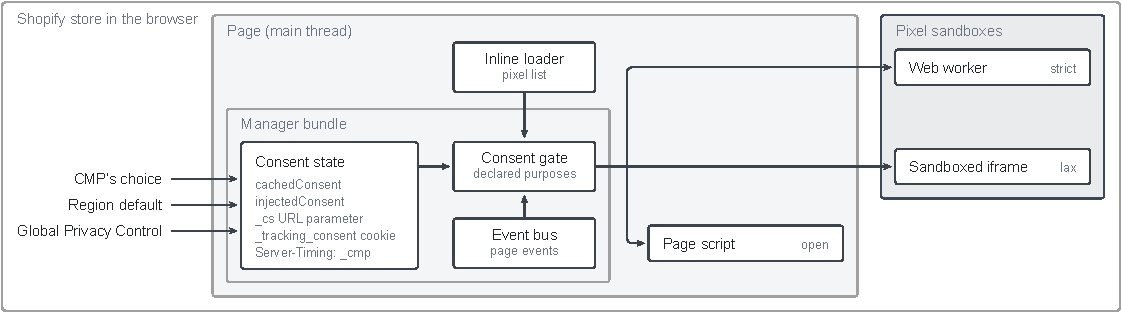
\includegraphics{figS1.pdf}
% GENERATED by paper/integrate_figures_v2.py from figures/v7/supp/caption_supp.tex (v2 figure caption, rendered by the figure script).
% Do not edit: change the figure script and re-run build.sh.
\caption{\textbf{Shopify's Web Pixels Manager (WPM) decides in the page's main thread whether a sandboxed pixel starts, and never stops it afterwards.} A schematic of our static reading of the WPM manager bundle and its inline loader (Methods), read from left to right and drawn like Fig.~1a: the outer frame is the Shopify store in the visitor's browser; inside it, the light grey ground is the page's main thread and the darker grey ground beside it the pixel sandboxes, which are isolated from the page; the outlined frame inside the page is the manager bundle. Boxes are components, with their secondary text in grey; arrows show what feeds what. Inline loader (top, in the page): each storefront page lists every pixel (`pixel list') with its type (`APP' or `CUSTOM'), its runtime context (`runtimeContext': `STRICT', `LAX' or `OPEN') and its declared privacy purposes (analytics, marketing, preferences, sale of data), so a crawler can read the list before any script runs; the list feeds the consent gate. Consent signals (left), in the order and words of Fig.~1a: the choice of a consent-management platform (CMP) that calls `setTrackingConsent'; the merchant's region default, written by the server into the page response; and, for sale of data only, Global Privacy Control (GPC), whose `Sec-GPC' request header makes the server decline sale of data. Manager bundle (middle): the consent state is the first one found of the sources listed in its box, in this order: `cachedConsent', `injectedConsent', the `\_cs' URL parameter, the `\_tracking\_consent' cookie and the `Server-Timing: \_cmp' header; if none can be read, everything is allowed. The event bus replays page events to every pixel, and each event carries the full page URL. The consent gate starts a pixel only when the consent state allows every purpose the pixel declares, and starts a pixel that declares no purpose at once. Runtime containers (right; the grey qualifier in each box is the runtime context): the gate starts each pixel in the container its runtime context names, a web worker (strict, `STRICT') or a sandboxed iframe (lax, `LAX'), both on the pixel sandboxes' ground, so a script blocker in the page cannot see them, or a script in the page (open, `OPEN'), drawn on the page's ground, which a blocker can see. In the web worker the vendor library sends with `fetch' without cookies, and `navigator' is overwritten, so pixel code reads GPC as undefined. We found no code path that stops a pixel once it has started. Schematic drawn in TikZ, with no generated imagery.
Drawn by figure-generation scripts written with AI assistance (Section~\ref*{M:sec:method-ai} of the main article).}
\label{fig:s1}

\end{widefig}

% ============================================================================
\section{Sample and crawl details}\label{sec:s-sample}
% ============================================================================

Table~\ref{tab:s-buckets} gives the frame and the sample by Tranco rank bucket, Table~\ref{tab:s-exclusions} the reasons for excluding verified domains and Table~\ref{tab:s-failures} the unusable loads of the crawl.

\begin{table}[!htbp]
\centering
\caption{Sampling frame and sample by Tranco rank bucket (list L5PZ4). Flagged: domains whose apex or \code{www} host resolved to Shopify's address block or a \code{myshopify.com} CNAME. Drawn: domains verified with one homepage request (census in the three upper buckets; seeded random order in the 100k--200k bucket). Live: verified Online Store storefronts before content exclusions, product-URL checks and de-duplication. Captured: usable loads in all three base arms. Weight: design weight $N_h/n_h$.}
\label{tab:s-buckets}
\small
\begin{tabular}{@{}lrrrrrrrr@{}}
\toprule
Bucket & Domains & Resolved & Flagged & Drawn & Live & Sample & Captured & Weight \\
\midrule
\tabinput{tables/supp_buckets.tex}
\bottomrule
\end{tabular}
\end{table}

\begin{table}[!htbp]
\centering
\caption{Reasons for excluding verified domains from the sample (first failing rule). The 21 stores flagged by the adult and child keyword screen were reviewed from their titles and descriptions without an independent human rater (Sections~\ref*{M:sec:method-sample} and~\ref*{M:sec:method-ai}).}
\label{tab:s-exclusions}
\small
\begin{tabular}{@{}lr@{}}
\toprule
Reason & Domains \\
\midrule
\tabinput{tables/supp_exclusions.tex}
\bottomrule
\end{tabular}
\end{table}

\emph{Frame and verification.} Each domain and its \code{www} host were resolved; Shopify's own platform domains were excluded. Of 219 hosts that our unpublished pilot study of creator links had identified as Shopify from page content, the DNS rule caught 190 (86.8\%); the misses sit behind the merchant's own CDN or a headless front end. Verification used the HTTP library's default user agent and no JavaScript, plus one request to the public product list for 176 sites whose homepage linked no product.

\emph{Frame recall.} After the crawl, the same verification code requested once the homepage of a seeded random sample of 600 resolving, non-flagged domains per bucket (19 domain names matching the adult or child keyword screen were not contacted). Of the 2,381 contacted, 1,480 returned an inspectable page (the others returned 403 or other errors, which may hide storefronts), and 4 of these were Online Store storefronts: 1, 0, 2 and 1 in the four buckets. Scaled to the non-flagged domains of each bucket and compared with the flagged storefronts, the estimated recall of the DNS rule is 23\% (5--63\%) in the 1--10k bucket, where 7 flagged storefronts face an estimated 23 missed ones, 100\% (at least 34\%) in the 10k--50k bucket, 73\% (43--91\%) in the 50k--100k bucket and 87\% (55--97\%) in the 100k--200k bucket, and about 83\% overall (bucket-wise bounds 48--96\%, not a joint interval); the intervals propagate only the Wilson interval of the missed-storefront rate. Separately, the \code{shop.} and \code{store.} subdomains of a seeded sample of 5,000 domains per bucket were resolved; 86, 67, 44 and 34 domains per bucket (231 in all) had a storefront there whose apex and \code{www} host were not flagged, confirmed by one homepage request to each of 301 flagged subdomains. Scaled up, about 1,828 such storefronts lie outside the frame, for example the merchandise stores of news, software and non-profit sites.

\emph{Landing page.} The landing page was the first same-host \code{/products/} link on the homepage or, failing that, the first handle in the public product list (136 stores). The rule does not choose a typical product: 126 of the 1,358 captured stores (9.3\%) landed on a gift card, gift voucher or gift certificate (5 further product URLs contain ``gift'' but are gift boxes or gifts), with a similar pre-choice outcome (a sandboxed ad request on 61.9\% of them against 58.8\% of the others), and a few sampled storefronts are not retailers (for example the site of a vendor of Shopify apps).

\emph{Crawler settings and canary.} Loads used locale en-US, time zone America/Los\_Angeles and a 1366$\times$900 viewport. The browser was visibly automated: every usable load's page probe read \code{navigator.webdriver} as true and a user agent containing ``HeadlessChrome'' (4,840 of 4,840 loads, including all 98 Brave loads, which also ran headless). CMPs were detected by script URLs, cookies and product-specific globals. A banner counted as visible if a CMP container or a fixed or dialog element with cookie or privacy wording held a visible clickable control and at least 20 characters of text, polled every 250~ms; the final detector, which replaced one that had counted an invisible Consentmo wrapper as a banner, was checked on 12 known stores, and the 510 loads judged by the first detector were re-run. In the Decline arm, Shopify's consent state was read 1~s and 5~s after the click, and the first page was observed for 15~s. Of the 63 changes of Shopify's marketing state to ``allowed'' in loads without a click, 60 came before the first passive scroll; the other 3, on two OneTrust stores, came 0.2--0.3~s after it. Counting every ``yes'' write without a click, whether or not it changed the state, 174 of 185 in Default and GPC loads came before the first scroll and 11 after one, on 8 stores and 175--797~ms after a scroll, so consent on scrolling cannot be excluded there. The canary set \code{utm\_source}, \code{utm\_medium} and \code{utm\_campaign} to \code{privacy-research}, \code{measurement} and \code{cmpstudy-<store\_id>}. Creator stores were loaded from the landing URL that the creator's link redirects to, with the token appended; because that URL already carried the creator's campaign parameters, it held duplicate \code{utm\_} keys.

\emph{Attribution details.} Each sandboxed or OPEN request is joined to its pixel's configuration entry; the join succeeded for 13,250 of 13,334 ad requests from STRICT workers and 18,097 of 18,169 from LAX iframes. LAX frames were identified by URL; in 200 sampled load records, none of the 764 LAX frames carried a recorded sandbox attribute, so the attribute and the opaque origin are inferred from Shopify's code. Vendors are the receivers of requests: 2 of 12 spot-checked STRICT requests were cookie synchronizations that an AppLovin pixel sent to a Google endpoint, and count as Google. An earlier, broader relay label (Shopify's manager anywhere in the initiator stack) covered 6,111 Default requests, of which 66.3\% had a vendor library in the stack, 31.8\% another third-party script, and only 1.9\% nothing but Shopify or store code; only the last now count as relayed, which lowers the share of ad requests that are sandboxed or relayed from 46.2\% to 31.8\%. Two corrections were made after review. CORS preflights of worker requests, which DevTools reports in the page's session where the crawler labelled them main-thread, are not ad requests (318 Default requests removed). Frames nested inside a LAX sandbox, which the crawler labelled by their own URL, count as sandboxed: following the saved frame tree moved 245 Default ad requests on 54 stores into the sandbox, and 52 whose frame URL the same load also used outside a sandbox were left out. No store-level sandboxed flag changed; with the crawler's own labels, the sandboxed share had been 30.6\% of 40,334 requests.

\emph{Instrumentation pause.} The crawler attached to every worker with \code{waitForDebuggerOnStart}, so each worker waited until its network capture was on. Over 30,064 workers in 4,615 usable loads the wait was a median 5~ms (90th percentile 64~ms, maximum 18,780~ms); for STRICT workers it was a median 6~ms (90th percentile 68~ms, maximum 2,333~ms), and 695 of 20,631 STRICT workers (3.4\%) waited longer than one banner-polling interval. The pause delays sandboxed requests, so ``pixel before banner'' is conservative; the race analysis times container creation, which the pause does not affect.

\emph{Load on stores.} The final crawl made 4,976 loads plus 257 next-page reloads; 510 earlier loads judged by the superseded banner detector and 19 first attempts that were retried add to the load that stores received. Per store this was 3 to 11 page loads; 42 stores received more than 7 and 34 received 10 or 11. Sampling made one homepage request to each of 1,518 domains, one product-list request to 176 of them and homepage checks of 44 creator candidates. Pilots and checks made 24 and 12 loads on a few stores, 5 Brave loads on one store and 3 static fetches of Shopify and Pandectes scripts; the records of two earlier pilot runs, a first 6-store pilot and a 12-store check of an intermediate banner detector, were deleted, so their load counts are not known. After an internal audit, the re-check crawl added one load to each of 129 stores (none to \storeC), and the \code{robots.txt} check one request to each of 1,433 stores; with the re-check, 43 stores received more than 7 page loads and none more than 11.

\emph{\code{robots.txt}.} The crawler did not consult \code{robots.txt}. Retrospectively, on 26 September 2026, we fetched it for every store we had loaded except \storeC, which we did not contact again: 1,427 of 1,433 stores served one. For the rules that apply to a crawler without its own product token, 20 stores disallowed the exact landing URL we loaded: 16 only because of the campaign parameters that carried our canary token (8 through rules that name \code{utm} parameters), and 4 because of the path, 2 of which disallow all crawling. The homepage requests of the sampling stage were disallowed on 2 stores and the product-list requests on none of 136.

\emph{Stores not captured.} Of the 38 analysed sampled stores not captured in all three base arms, 23 redirected our browser to google.com, 9 had lost their product page, 3 lacked Shopify's page object, 2 did not resolve and 1 was unavailable. None was in the top bucket; they were 9 of 180 stores (5.0\%) in the 10k--50k bucket, 13 of 634 (2.1\%) in the 50k--100k bucket and 16 of 575 (2.8\%) in the 100k--200k bucket. A consent tool was detected in at least one of their loads on 19 of the 38, against 789 of the 1,358 captured stores; the tools seen most often were Shopify's own banner (7), OneTrust (4) and Consentmo (3), and none used Pandectes. The losses are therefore small and not concentrated in one consent tool.

\emph{Creator stratum.} Our unpublished pilot study of creator links identified 219 Shopify store hosts. For 175 of them no link qualified: 102 had only links through an affiliate network or with a click identifier, 39 had no token or only an opaque one, 33 were creator-owned stores without a token in the URL, and one was Shopify's own site. Of the remaining 44 candidates, a homepage check excluded 10 (7 headless, 1 without Shopify markers, 1 blocked and 1 rate-limited), leaving 34 stores, 6 of them with a token that names a single video. Three creator stores are also in the main sample.

\begin{table}[!htbp]
\centering
\caption{Unusable loads by reason. Nothing was done to get around blocking or redirects.}
\label{tab:s-failures}
\small
\begin{tabular}{@{}lr@{}}
\toprule
Reason & Loads \\
\midrule
\tabinput{tables/supp_failures.tex}
\bottomrule
\end{tabular}
\end{table}

Table~\ref{tab:s-arms} defines each measurement arm: the privacy signal, the action, the window observed and the number of loads (drawn in Fig.~\ref*{M:fig:methods}c of the main article).

% tableS_arms.tex -- GENERATED by figures/v7/fig2/scripts/make_table_arms.py from analysis/outputs/stats.json
% and figures/v7/fig2/derived_numbers.json (registry: figures/v7/fig2/tableS_arms_numbers.csv); do not edit
% by hand. Supplementary Table S-arms (label tab:s-arms): % tableS_arms.tex -- GENERATED by figures/v7/fig2/scripts/make_table_arms.py from analysis/outputs/stats.json
% and figures/v7/fig2/derived_numbers.json (registry: figures/v7/fig2/tableS_arms_numbers.csv); do not edit
% by hand. Supplementary Table S-arms (label tab:s-arms): % tableS_arms.tex -- GENERATED by figures/v7/fig2/scripts/make_table_arms.py from analysis/outputs/stats.json
% and figures/v7/fig2/derived_numbers.json (registry: figures/v7/fig2/tableS_arms_numbers.csv); do not edit
% by hand. Supplementary Table S-arms (label tab:s-arms): \input{tables/tableS_arms.tex} in supplement.tex.
\begin{table}[!htbp]
\centering
\caption{Measurement arms (drawn in Fig.~2c). Every load used a new browser with a new temporary profile: Chromium's headless shell (version 149) in all arms but Brave (version 150, also headless). Repeats: a seeded 20\% subsample; Brave: a seeded 100-store subsample. Loads run and usable loads include the 34 creator-linked stores. Stores analysed: main-sample stores with usable loads in all three base arms (base arms), or in both loads of a comparison (validation rows: Default and GPC against their repeats, GPC against Brave; Fig.~6d). The arms are compared on equal 10~s windows: from the load event in Default and GPC, and on the next page in Decline (Fig.~5a).}
\label{tab:s-arms}
\small
\begin{tabularx}{\textwidth}{@{}>{\raggedright\arraybackslash}p{27mm}>{\raggedright\arraybackslash\hsize=1.2\hsize}X>{\raggedright\arraybackslash}X>{\raggedright\arraybackslash\hsize=0.8\hsize}X@{\hspace{6pt}}r@{\hspace{6pt}}r@{\hspace{6pt}}r@{}}
\toprule
 & & & Window & Loads & Usable & Stores \\
Arm & GPC signal & Action & observed & run & loads & analysed \\
\midrule
Default \mkDefault{} & none & none; passive mouse-wheel scrolls from 2~s after the \code{load} event & until 15~s after the \code{load} event & 1,434 & 1,397 & 1,358 \\[3pt]
Decline \mkDecline{} & none & waited for a visible banner and clicked its first-layer reject control (never Accept or settings); clicked on 240 stores, worked on 231; no click without such a control & before the click; same page after the click; next page (same URL reloaded, new sandboxes) for 10~s after its \code{load} event & 1,434 & 1,396 & 1,358 \\[3pt]
GPC \mkGPC{} & \code{Sec-GPC:~1} on every request; \code{navigator.globalPrivacyControl} injected into every frame and worker before its first script & as Default & as Default & 1,434 & 1,397 & 1,358 \\
\addlinespace
Default repeat \mkRepeat{} & none & as Default & as Default & 287 & 284 & 273 \\
GPC repeat \mkRepeat{} & as GPC & as Default & as Default & 287 & 284 & 273 \\
Brave \mkRepeat{} & Brave's native GPC; Shields (tracker blocking) off & as Default & as Default & 100 & 99 & 98 \\
\bottomrule
\end{tabularx}
\end{table}
 in supplement.tex.
\begin{table}[!htbp]
\centering
\caption{Measurement arms (drawn in Fig.~2c). Every load used a new browser with a new temporary profile: Chromium's headless shell (version 149) in all arms but Brave (version 150, also headless). Repeats: a seeded 20\% subsample; Brave: a seeded 100-store subsample. Loads run and usable loads include the 34 creator-linked stores. Stores analysed: main-sample stores with usable loads in all three base arms (base arms), or in both loads of a comparison (validation rows: Default and GPC against their repeats, GPC against Brave; Fig.~6d). The arms are compared on equal 10~s windows: from the load event in Default and GPC, and on the next page in Decline (Fig.~5a).}
\label{tab:s-arms}
\small
\begin{tabularx}{\textwidth}{@{}>{\raggedright\arraybackslash}p{27mm}>{\raggedright\arraybackslash\hsize=1.2\hsize}X>{\raggedright\arraybackslash}X>{\raggedright\arraybackslash\hsize=0.8\hsize}X@{\hspace{6pt}}r@{\hspace{6pt}}r@{\hspace{6pt}}r@{}}
\toprule
 & & & Window & Loads & Usable & Stores \\
Arm & GPC signal & Action & observed & run & loads & analysed \\
\midrule
Default \mkDefault{} & none & none; passive mouse-wheel scrolls from 2~s after the \code{load} event & until 15~s after the \code{load} event & 1,434 & 1,397 & 1,358 \\[3pt]
Decline \mkDecline{} & none & waited for a visible banner and clicked its first-layer reject control (never Accept or settings); clicked on 240 stores, worked on 231; no click without such a control & before the click; same page after the click; next page (same URL reloaded, new sandboxes) for 10~s after its \code{load} event & 1,434 & 1,396 & 1,358 \\[3pt]
GPC \mkGPC{} & \code{Sec-GPC:~1} on every request; \code{navigator.globalPrivacyControl} injected into every frame and worker before its first script & as Default & as Default & 1,434 & 1,397 & 1,358 \\
\addlinespace
Default repeat \mkRepeat{} & none & as Default & as Default & 287 & 284 & 273 \\
GPC repeat \mkRepeat{} & as GPC & as Default & as Default & 287 & 284 & 273 \\
Brave \mkRepeat{} & Brave's native GPC; Shields (tracker blocking) off & as Default & as Default & 100 & 99 & 98 \\
\bottomrule
\end{tabularx}
\end{table}
 in supplement.tex.
\begin{table}[!htbp]
\centering
\caption{Measurement arms (drawn in Fig.~2c). Every load used a new browser with a new temporary profile: Chromium's headless shell (version 149) in all arms but Brave (version 150, also headless). Repeats: a seeded 20\% subsample; Brave: a seeded 100-store subsample. Loads run and usable loads include the 34 creator-linked stores. Stores analysed: main-sample stores with usable loads in all three base arms (base arms), or in both loads of a comparison (validation rows: Default and GPC against their repeats, GPC against Brave; Fig.~6d). The arms are compared on equal 10~s windows: from the load event in Default and GPC, and on the next page in Decline (Fig.~5a).}
\label{tab:s-arms}
\small
\begin{tabularx}{\textwidth}{@{}>{\raggedright\arraybackslash}p{27mm}>{\raggedright\arraybackslash\hsize=1.2\hsize}X>{\raggedright\arraybackslash}X>{\raggedright\arraybackslash\hsize=0.8\hsize}X@{\hspace{6pt}}r@{\hspace{6pt}}r@{\hspace{6pt}}r@{}}
\toprule
 & & & Window & Loads & Usable & Stores \\
Arm & GPC signal & Action & observed & run & loads & analysed \\
\midrule
Default \mkDefault{} & none & none; passive mouse-wheel scrolls from 2~s after the \code{load} event & until 15~s after the \code{load} event & 1,434 & 1,397 & 1,358 \\[3pt]
Decline \mkDecline{} & none & waited for a visible banner and clicked its first-layer reject control (never Accept or settings); clicked on 240 stores, worked on 231; no click without such a control & before the click; same page after the click; next page (same URL reloaded, new sandboxes) for 10~s after its \code{load} event & 1,434 & 1,396 & 1,358 \\[3pt]
GPC \mkGPC{} & \code{Sec-GPC:~1} on every request; \code{navigator.globalPrivacyControl} injected into every frame and worker before its first script & as Default & as Default & 1,434 & 1,397 & 1,358 \\
\addlinespace
Default repeat \mkRepeat{} & none & as Default & as Default & 287 & 284 & 273 \\
GPC repeat \mkRepeat{} & as GPC & as Default & as Default & 287 & 284 & 273 \\
Brave \mkRepeat{} & Brave's native GPC; Shields (tracker blocking) off & as Default & as Default & 100 & 99 & 98 \\
\bottomrule
\end{tabularx}
\end{table}


\emph{GPC injection into workers.} In the Chromium build we used, evaluating a script in a worker that is paused at start crashed the renderer. The crawler therefore set a debugger instrumentation breakpoint before the worker's first script, resumed the worker, injected \code{navigator.globalPrivacyControl = true} when it paused, removed the breakpoint and resumed again. A local test page with the same container types as Shopify (a sandboxed iframe with an opaque origin, a dedicated worker created with \code{credentials:'omit'}, a nested worker and a blob worker created inside the sandboxed iframe) read the flag as true in the first statement of every target in 20 of 20 runs, with the \code{Sec-GPC} header on the worker script, \code{importScripts} and \code{fetch} requests; a control without injection read true in 0 of 3 runs. The technique is not needed to test Shopify's gate, because STRICT pixel code cannot read the flag (Section~\ref*{M:sec:app-validation}), but it may be reused on worker-heavy pages elsewhere.

\emph{Brave with Shields off.} Each Brave load wrote a preference that switches Shields off into its new temporary profile; the user's own browser profiles were never used. A local positive control confirmed the setting: with default Shields, Brave randomized \code{hardwareConcurrency} and canvas output, and with the preference set it returned the true values in 3 of 3 runs. In the crawl, no request was blocked by the client, and Brave's filter lists were never downloaded into these profiles.

% ============================================================================
\section{Consent tools}\label{sec:s-cmp}
% ============================================================================

\emph{Readable declared policies.} For Pandectes (versions 4 and 5) we read the blocklist of URL patterns per category and the categories blocked by default. Version 5 applies its opt-in rules only to regions listed as strict; California was a strict region on 5 of the 39 stores running version 5, and only on those stores do we count a version-5 blocklist entry as declared blocked before any choice (3 of the 21 blocklist stores of Section~\ref*{M:sec:res-paper}; the other two are a creator store and a store without an ad vendor on its list). For OneTrust we read the URL-to-category map of its auto-blocking script and compared it with the active consent groups; this map is empty when the script fails to load. For Cookiebot we read the tag configuration and the blocking mode. Other products were detected but their declared lists could not be read reliably, which is why the main sample's blocklist stratum holds 21 stores and the expansion (\ref{sec:s-r4}) was screened for these products only.

Table~\ref{tab:s-cmp} and Fig.~\ref{fig:s2} give the outcomes per consent tool.

\emph{Integration modes are capabilities.} A product that can write to Shopify's Customer Privacy API may not do so on a given store, for example when the merchant installed it without the product's Shopify app or before the vendor enabled the integration. The crawler therefore tested each store: after a working Decline click, did Shopify record an explicit refusal?

\emph{Blocked-on-paper details.} The declared lists are store-specific: the 15 Pandectes stores carried 14 distinct sets of blocked ad vendors, and the 5 OneTrust stores 5. The declared vendor fired from the sandbox on 9 of the 15 Pandectes, 3 of the 5 OneTrust and 0 of the 1 Cookiebot store, and in the primary sample on 4 of 8, 3 of 5 and 0 of 1; the 15 stores whose blocklist shares one product's Shopify integration are not independent draws.

\emph{Stores whose CMP wrote ``yes''.} A blocklist is in force for a visitor only while the CMP has not consented. On 7 of the 21 stores, all using Pandectes, the CMP wrote ``marketing: yes'' in the Default load without any click. Two run version 5 and match its optional bot setting (Section~\ref*{M:sec:app-validation}). The other 5 run version 4, whose code was not saved, so its mode cannot be read from code; version 5 applies an ``optout'' policy, in which consent is implied, outside its strict regions. On 2 of these stores no banner was shown in California and the CMP wrote ``yes'' within about a second, as such an implied-consent mode would; on 2 the banner was shown and the ``yes'' came with it, before any scroll; and on 1 it came just after our first passive scroll. All 7 are excluded from the primary estimate. The 7 version-4 stores without a ``yes'' never recorded consent, so their blocklists were in force; the declared vendor fired on 4 of them. Other exclusion rules give 9 of 17 (without the 4 stores whose CMP switched a denying default to ``yes'') and 9 of 16 (without every store whose ``yes'' came before the declared vendor's pixel). Among stores with a configured sandboxed pixel of a declared vendor, the vendor fired on 10 of 15, and on 6 of 11 in the primary sample; on 4 of the 21 stores no declared vendor had a sandboxed pixel at all.

\emph{Stratified and like-for-like comparisons.} Over all 21 stores, the declared vendor fired from the sandbox on 8 of 10 blocklist stores whose default allowed marketing (against 123 of 174, 70.7\%, of banner stores with no readable declaration and the same default) and on 4 of 11 whose default denied it (against 40 of 167, 24.0\%, of all ``denied until consent'' banner stores). On the 4 denied-default stores whose CMP wrote ``yes'' before any click, a sandboxed ad pixel fired on all 4 (the declared vendor itself on 3). Comparing any sandboxed ad pixel like for like over all stores, including those whose CMP wrote ``yes'', blocklist stores fired on 9 of 10 against 123 of 174 where the default allowed and on 6 of 11 against 36 of 158 where it denied (Mantel--Haenszel difference 25.8 percentage points, 95\% CI 8.0 to 43.6); among stores whose CMP wrote no ``yes'' the difference was 13.6 percentage points (95\% CI $-8.4$ to 35.6). Neither shows a reduction. With the expansion (\ref{sec:s-r4}), the primary comparison of the main article, on the stores of both samples whose CMP wrote no ``yes'', gives 13.4 percentage points (95\% CI 4.0 to 22.8), and the comparison over all stores 21.3 percentage points (95\% CI 12.8 to 29.8).

\emph{Pattern-level match (exploratory).} For 13 of the 18 Pandectes entries whose vendor fired from the sandbox, on 8 stores (3 of them in the primary sample), the CMP's own blocklist pattern matched a URL that the STRICT worker fetched in the Default load; the matching vendors were mostly Microsoft UET (5 entries) and TikTok (3).

\emph{Re-check of the blockers.} In the re-check load, a blocker neutralized at least one element on all 15 Pandectes stores, the Cookiebot store and 2 of the 5 OneTrust stores. Of the 12 stores where the declared vendor had fired from the sandbox in the main crawl, the blocker was active on 10, and the vendor fired from the sandbox again on 11. The other 2 are OneTrust stores (S0589, S0698) on which no element was neutralized at all: OneTrust's declaration rests on a URL-to-category map that may not have been enforced there. On 5 stores (S0165, S0213, S0219, S0370, S0697; none a bot-rule store) the blocker neutralized a main-document tag of a declared-blocked vendor in the same load in which that vendor's pixel sent requests from Shopify's sandbox. A main-document tag was seen for only 22 of the 104 entries, so most entries named tags that the page did not load in that visit. Blocker activity was not logged in the main crawl.

\emph{Other entries.} Of the 75 declared entries for which no configured sandboxed pixel of the vendor was identified (classic tags, OPEN pixels or installation unknown), 15 fired by any route: 4 from a Shopify sandbox through a pixel that we could not map to the vendor, 4 through Shopify's OPEN pixel, whose injected script a blocker can see, and 7 from ordinary page scripts.

\emph{Detection and automation rules by tool.} Table~\ref{tab:s-detection} gives, per consent tool, the stores on which it was detected, those on which its banner was shown in the Default load, and the rule reacting to automated browsers that we found in its saved code. Consentmo was detected on 104 stores but showed a banner on 1; its container was present but empty (\ref{sec:s-audit}), and its saved code has no rule for bots, so geo-targeting of the banner away from California is the likely explanation. Didomi was detected on 14 stores and showed a banner on none, although its banner element was present but hidden on 11.

\begin{table}[!htbp]
\centering
\caption{Consent tools detected in the Default load (tools detected on at least 5 stores): stores on which the tool was detected, on which its banner was shown, and on which its banner element was present but hidden, with the rule reacting to automated browsers that we found in the tool's saved code (``code not saved'': no copy of the tool's code was kept).}
\label{tab:s-detection}
\footnotesize
\tabinput{tables/tableS_cmp_detection.tex}
\end{table}

\begin{table}[!htbp]
\centering
\caption{Outcomes by consent tool (the CMP that showed the banner in the Default load; ``Other or none'' includes stores without a detected CMP). Cells give $k/n$ and, for $n\ge5$, the percentage. Banners: stores with a banner in the Default load (409 in all). Default denies: Shopify's region default denies marketing, among banner stores with a readable default. Pre-choice: a sandboxed ad request before any choice, among banner stores. Reject: a first-layer reject control, among stores where the Decline arm found a banner. Refusal: Shopify recorded an explicit refusal, among working clicks. Fresh page: a new sandbox sent an ad request on the next page, among working clicks. GPC: a sandboxed ad request under GPC, among the stores assigned to the tool that had one under Default; stores are assigned to the CMP that showed the banner or, where none did, to the CMP detected, so this column also counts stores without a banner (for Shopify's banner, 165 stores with a sandboxed request under Default, against 68 banner stores). Mode: integration mode (Table~\ref*{M:tab:cmp-modes}). Rates describe the stores that use each tool, not the tool's quality.}
\label{tab:s-cmp}
\footnotesize\setlength{\tabcolsep}{3pt}
\begin{tabular*}{\textwidth}{@{\extracolsep{\fill}}llrrrrrrr@{}}
\toprule
Consent tool & Mode & Banners & Default denies & Pre-choice & Reject & Refusal & Fresh page & GPC \\
\midrule
\tabinput{tables/supp_per_cmp.tex}
\bottomrule
\end{tabular*}
\end{table}

\begin{widefig}
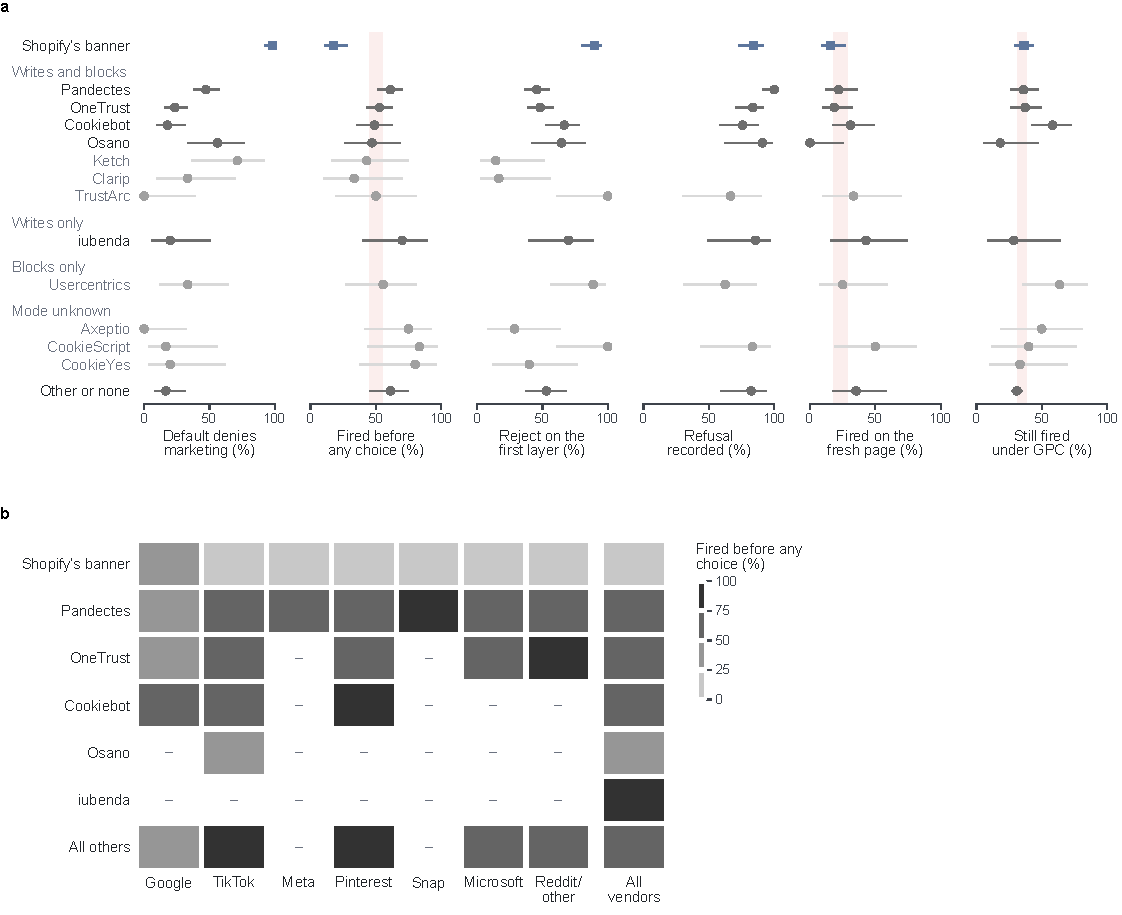
\includegraphics{figS2.pdf}
% GENERATED by paper/integrate_figures_v2.py from figures/v7/supp/caption_supp.tex (v2 figure caption, rendered by the figure script).
% Do not edit: change the figure script and re-run build.sh.
\caption{\textbf{Shopify's own banner had the lowest pre-choice firing of any consent tool and also the most denying region defaults, so the tools cannot be ranked on these data.} (a)~Six outcomes per consent-management platform (CMP), the tool that showed the banner in the Default load. The rows are grouped by the tool's integration mode, each group set apart by a gap and the four mode groups of third-party tools named by a grey header; from top to bottom: Shopify's own banner; tools that both write the choice to Shopify and block tags in the page's main thread (`Writes and blocks': Pandectes, OneTrust, Cookiebot, Osano, Ketch, Clarip and TrustArc); a tool that writes to Shopify only (`Writes only': iubenda); a main-thread blocker only (`Blocks only': Usercentrics); tools whose mode is unknown (`Mode unknown': Axeptio, CookieScript and CookieYes); and other or no detected tool. One dot plot per outcome, the tools sharing rows; from left to right: Shopify's region default denies marketing (banner stores with a readable default) and a sandboxed ad request before any choice (banner stores), both in the Default load; a reject control on the banner's first layer (stores where the Decline load found a banner), Shopify recorded an explicit refusal (working clicks) and a new sandbox sent an ad request on the fresh page after Decline (working clicks), all three in the Decline load; and a sandboxed ad request still sent under Global Privacy Control (GPC; stores with one under Default, assigned to the tool that showed the banner or else the one detected, so the last row also counts stores without a banner). Marks: share of stores; lines: Wilson 95\% confidence intervals (CIs), in the colour of their mark. Shopify's own banner, the row the title is about, is drawn as slate squares; every other tool is context, drawn as grey circles, and tools with fewer than 10 banner stores are drawn lighter (light grey circles and intervals, names in grey), as the top rank bucket of Fig.~S3. The plots of the three rates that Fig.~S5 tests (fired before any choice, fired on the fresh page and still fired under GPC) carry a pale brick band: that rate over all tools, which is the main estimate of Fig.~S5 with its Wilson 95\% CI (the tools' rows pool to it), so each tool reads against the overall rate. Cells with fewer than 5 stores are not drawn. Shopify's own banner: the region default denied marketing on 65 of 66 stores (98.5\%) and a sandboxed ad request preceded any choice on 12 of 68 (17.6\%). The $k$ and $n$ of every cell are in Table~\ref{tab:s-cmp}. (b)~Share of configured sandboxed vendor pixels that sent an ad request before any choice, by consent tool (rows, in the order of (a)) and vendor group (columns), among banner stores whose Shopify configuration lists the vendor's pixel, in four equal grey steps from light (low) to dark (high; thin colour bar at right), the cells split by thin white gaps; the lightest step is a definite grey, so it never reads as white. The column set apart at the right, `All vendors', counts the store--vendor pairs of every group. By row, the pairs that fired: Shopify's banner 14 of 141 pairs (68 banner stores); Pandectes 124 of 202 (95); OneTrust 76 of 142 (91); Cookiebot 43 of 70 (45); Osano 21 of 46 (17); iubenda 14 of 18 (10); all other tools 99 of 145 (83); in all 391 of 764 pairs (51.2\%). Blank cells with a grey dash: fewer than 10 banner stores configure the vendor's pixel (often none), so no rate is shown; a dash means no estimate, not a low rate. Rates describe the stores that use each tool, not the tool's quality.}
\label{fig:s2}

\end{widefig}

% ============================================================================
\section{Results by Tranco rank bucket}\label{sec:s-rank}
% ============================================================================

Figure~\ref{fig:s3} repeats the headline rates by Tranco rank bucket.

\begin{widefig}
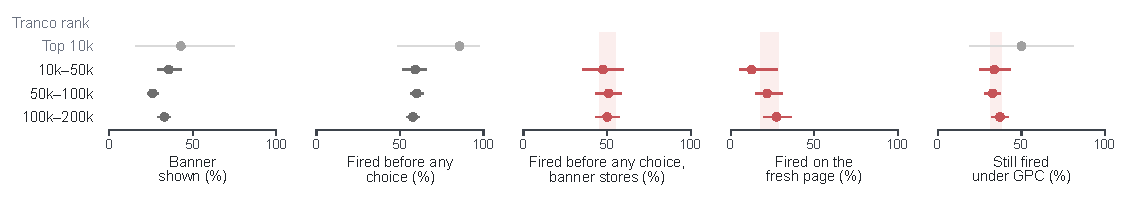
\includegraphics{figS3.pdf}
% GENERATED by paper/integrate_figures_v2.py from figures/v7/supp/caption_supp.tex (v2 figure caption, rendered by the figure script).
% Do not edit: change the figure script and re-run build.sh.
\caption{\textbf{Pre-choice firing on banner stores was about the same in every Tranco rank bucket below the top one.} Outcomes by Tranco rank bucket (rows, top to bottom): the top 10k ranks (7 captured stores), 10k--50k (171), 50k--100k (621) and 100k--200k (559), unweighted. One dot plot per outcome, the buckets sharing rows; from left to right: a banner shown, and a sandboxed ad request before any choice among all stores and among banner stores (Default load); a new sandbox sent an ad request on the fresh page after a working Decline; a sandboxed ad request still sent under Global Privacy Control (GPC; stores with one under Default). The rows are named once, under the grey header `Tranco rank'. Circles: share of stores; lines: Wilson 95\% confidence intervals (CIs), in the colour of their mark. The last three plots show the three rates that Fig.~S5 tests, all rates at which consent was lost, and are drawn alike: brick circles on a pale brick band, which is that rate over all four buckets, the main estimate of Fig.~S5 with its Wilson 95\% CI (the buckets pool to it); the first two plots are context, in grey. The top bucket holds only 7 stores (fewer than 10) and is drawn lighter in every plot (light grey circles and intervals, its name in grey), as the small tools of Fig.~S2a (in Fig.~S5, by contrast, grey marks a changed definition of the measure). Cells with fewer than 5 stores are not drawn. $k$ of $n$ by bucket, top to bottom. Banner shown: 3 of 7; 61 of 171; 161 of 621; 184 of 559. Before any choice, all stores: 6 of 7; 101 of 171; 373 of 621; 323 of 559. Before any choice, banner stores (47.5--50.9\% in the three lower buckets): 2 of 3 (not drawn); 29 of 61; 82 of 161; 92 of 184. Fresh page: 0 of 1 (not drawn); 4 of 32; 20 of 92; 29 of 106. Under GPC: 3 of 6; 34 of 101; 122 of 373; 120 of 323.}
\label{fig:s3}

\end{widefig}

% ============================================================================
\section{Screenshot audits and repeat agreement}\label{sec:s-audit}
% ============================================================================

The screenshot audit covers a seeded random sample of 54 Decline loads (36 clicked, 18 without a first-layer reject option) and, separately, all 12 forced clicks. The forced-click audit found 10 modals or gates (e-mail, location or age) and 1 chat widget over the banner, and agreed with the rule for a working click on all 12. One clicked control was labelled ``Limit''; the crawl record shows that it was OneTrust's reject-all control (\code{\#onetrust-reject-all-handler}), that the banner was gone after the click, that every non-necessary OneTrust group was then off and that Shopify recorded ``no'' for all purposes, so no Accept-type control was clicked. All labels were made from the saved screenshots without an independent human rater (Section~\ref*{M:sec:method-ai}); a blind re-labelling has not yet been done.

\emph{Recall re-check.} Because only loads with a detected banner have Decline screenshots, the recall of the banner detector was audited with a re-check crawl on 26 September 2026 (15:33--15:41~UTC; Section~\ref*{M:sec:method-validation}). It loaded 128 analysed main-sample stores once more with the same browser, pacing and landing URL and no interaction at all, not even scrolling (the browser again read \code{navigator.webdriver} as true and sent a ``HeadlessChrome'' user agent, in 127 of 127 usable loads, so banners that a tool hides from bots cannot be found this way): the 79 stores on which Shopify's \code{shouldShowBanner()} had been true while no banner was detected, a seeded random sample of 30 of the 870 other stores without a detected banner, and the 21 blocklist stores (two stores were in two groups). It saved the viewport at about 3, 6 and 10~s after the \code{load} event and logged every script and iframe element added to the page, with every later change of its \code{type} or \code{src} attribute, to record which tags a blocker neutralized. The screenshots were shown in a seeded random order under neutral codes, three per store, 5 stores per sheet, without group, consent tool or detector result, and labelled without an independent human rater (Section~\ref*{M:sec:method-ai}); small notice bars were checked in a second pass on the top and bottom strips of the 3~s and 10~s shots of every store labelled ``no''. Newsletter, discount, country and survey pop-ups were not counted as consent banners. A banner that the main crawl had not detected was visible on 10 of 78 flagged stores and 1 of 30 random stores (one flagged load produced no screenshot). None of the 53 flagged Consentmo stores with screenshots showed one: Consentmo's container was present but empty, as it had been for the superseded detector, so these stores were correctly counted as having no banner. Most of the missed banners came from a consent tool outside our signature list (4 of the 10 that the detector also missed on the re-check load were \code{dg-consent-banner} elements); on the re-check loads, the detector found 18 of the 28 visible banners and raised no false alarm (18 of 18). Applying the random sample's rate (1 of 30, 95\% CI 0.6--16.7\%) to the 870 other stores without a detected banner gives about 39 missed banners in the main crawl (15--155), a recall of about 91\% (73--96\%), if a banner seen on the re-check was also shown in the original load. Counting the 11 banners found as banner stores changes the projection of Section~\ref*{M:sec:app-projection} from 15.7\% to 16.0\%; counting all 54 flagged Consentmo stores as banner stores, the worst case before the re-check, gives a banner-store rate of 46.4\% (41.9--51.0\%; Fig.~\ref{fig:s5}). The 11 stores were not clicked in the Decline arm.

\begin{widefig}
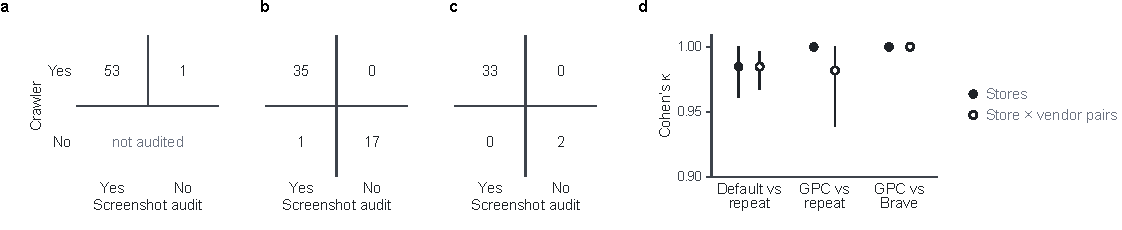
\includegraphics{figS4.pdf}
% GENERATED by paper/integrate_figures_v2.py from figures/v7/supp/caption_supp.tex (v2 figure caption, rendered by the figure script).
% Do not edit: change the figure script and re-run build.sh.
\caption{\textbf{The crawler's banner, reject and click labels agreed with screenshots in almost every audited load, and repeated loads agreed almost perfectly.} (a--c)~Crawler label (rows, shared by the three matrices and named once, left of (a)) against a screenshot audit (columns) in 54 seeded Decline loads (36 clicked, 18 without a reject option), as matrices of loads split into cells by crossing rules, as in Fig.~S7b; the diagonal (top left and bottom right): the crawler and the audit agree; the other two cells: they disagree. (a)~Banner detection: 53 of 54 detected banners were real (the exception was an age gate); the audit sampled only loads with a detected banner, so the crawler's `no' row was not audited (one merged row, marked `not audited'). (b)~Reject option on the banner's first layer: agreement in 52 of 53 loads (one reject button in Romanian was missed). (c)~Whether the Decline click dismissed the banner, in the 35 clicked loads whose screenshot showed a banner: 35 of 35. The audit labels have not yet been checked by an independent human rater. (d)~Cohen's $\kappa$ for whether a sandboxed ad request fired, between a load and its repeat (Default; Global Privacy Control, GPC) and between emulated GPC and Brave's native GPC, per store (filled circles) and per store $\times$ vendor pair (open circles); lines: 95\% confidence intervals from a bootstrap that resamples stores; a comparison without any disagreement has a degenerate interval and no line. Note the truncated $\kappa$ axis, which does not start at zero; it runs a little past one, so the marks at $\kappa = 1$ have air above them. The key sits right of the plot. Default vs repeat: $\kappa$ 0.985 (0.961--1.000), 271 of 273 stores agreeing, and 0.985 (0.967--0.997), 1,902 of 1,911 pairs; GPC vs repeat: 273 of 273 stores ($\kappa$ 1.000) and $\kappa$ 0.982 (0.939--1.000), 1,908 of 1,911 pairs; GPC vs Brave: 98 of 98 stores and 686 of 686 pairs ($\kappa$ 1.000 for both). Default and GPC differed on 39 of the 98 Brave stores and on 109 of 686 store $\times$ vendor pairs, and Brave matched GPC on all of them. Counts of sandboxed ad requests per store also repeated: Spearman's $\rho$ 0.982 (0.957--0.999) for Default and 0.999 (0.995--1.000) for GPC (273 stores; bootstrap over stores).}
\label{fig:s4}

\end{widefig}

% ============================================================================
\section{Decline, GPC and timing details}\label{sec:s-decline}
% ============================================================================

\emph{Recording the Decline.} An earlier flag, \code{marketingAllowed()} false at the end of the Decline load, was true on 200 of 240 clicked stores, but on 105 of them the region default already denied marketing before the click; on the 11 ``denied until consent'' stores where it was not set, the state was unreadable, not ``yes''. The main article therefore uses the explicit refusal recorded after a working click.

\emph{Decline outcomes.} On the 117 stores whose default allowed marketing, the click turned it off on 93 (79.5\%, 71.3--85.8\%). Of the 101 stores with a sandboxed request before the click, 50 (49.5\%) had a new one on the fresh page, and where the state was unknown after the click, 3 of 15 did. On the 231 stores with a working click, the share with a sandboxed ad request in the first 10~s was 45.9\% under Default and 17.7\% under GPC (TikTok: 19.9\% and 1.3\%).

\emph{After the click.} On the same page, a sandboxed ad request followed the click on 32 of the 231 working clicks. After a recorded refusal, marketing-declaring pixels started before the click sent 46 requests on 15 stores, a median 918~ms and up to 9,088~ms after the click; 9 of these were issued by the pixel's own code under Shopify's sandbox, 12 by the vendor's library and 25 had no initiator stack, so the stacks cannot separate events that Shopify delivered after the opt-out from the vendor's own timers. On the reload, old sandboxes sent unload beacons on 30 of the 231 working-click stores (28 of them among the 196 with a recorded refusal): 50 requests, 47 of them Microsoft UET beacons, sent 15.1--16.2~s after the click and a median 0.25~s after the reload began; any real navigation away from the page triggers such beacons.

\emph{Residual classes after a recorded refusal.} Fig.~\ref{fig:s8}c (one class per store: Fig.~\ref*{M:fig:choices}b of the main article) classes each residual request by the purposes its pixel declares and by Shopify's state when the pixel started (for pixels started before the click, the reading after the click). Pixels declaring a refused purpose kept sending on 32 of the 196 stores, on the same page on 19 and through unload beacons on 20; new sandboxes of such pixels fired on none. Pixels declaring only purposes that the Decline left allowed fired on 13 stores: after the refusal, Shopify's state still allowed sale of data on 112 of the 196 stores. Pixels declaring no purpose fired on 28. On the fresh page (37 stores) the classes were no purpose on 27 stores (custom pixels 24, app pixels 4) and left allowed on 13 (custom 12, app 2); custom pixels were involved on 34 of the 37 stores and app pixels on 6. Split by the marketing declaration alone, as in an earlier version of this analysis, marketing-declaring and other pixels tied on the same page (15 stores each), unload beacons came from marketing-declaring pixels on 20 stores and from others on 9, and a marketing-declaring pixel kept sending on 29 stores against 43 on which a pixel not declaring marketing sent in some window (8 both).

\emph{Automatic writes.} The banners' automatic ``no'' writes came a median 1,630~ms after navigation start, and the first third-party marketing sandbox a median 829~ms. In the Default arm, a CMP wrote ``yes'' without a click on 22 of the 246 ``denied until consent'' stores (8.9\%, 6.0--13.2\%). On 9 of these 22 no banner was detected: 3 are stores matching Pandectes' bot setting (Section~\ref*{M:sec:app-validation}), and 6 are unexplained. Some automatic ``yes'' writes are therefore a CMP's reaction to an automated browser rather than behaviour a visitor would meet.

\emph{GPC.} Counting data beacons only, 242 of the 769 stores with a sandboxed beacon under Default still sent one under GPC. The navigation's consent string declined sale of data on 867 of the 869 GPC loads whose sale-of-data-region field was unset and on 479 of the 480 where it was set, so Shopify applied GPC regardless of that field. Under GPC the residual came from custom pixels only on 182 of the 279 stores, from app pixels only on 79 and from both on 17; pixels declaring only purposes that GPC leaves allowed fired on 111 of the 1,354 stores (marketing on 100) and pixels declaring no purpose on 191. The denominator of 1,354 stores in Figs.~\ref*{M:fig:choices}b and~\ref{fig:s8}c counts stores where either the navigation's consent string (1,341 stores) or a Customer Privacy API reading (1,166 of 1,169 loads with a readable state) showed ``sale of data: no''.

\emph{Timing.} The paired gap between banner visibility and the first sandboxed request had a median of 286~ms (interquartile range $-46$ to 859~ms). Counting data beacons only, the first beacon preceded the banner on 135 of 200 stores, by more than one polling interval on 94. Between repeat loads, the first request shifted by a median of 414~ms and the banner by 291~ms. The first request preceded the banner on 17 of 19 stores in the six-browser segment and on 132 of 184 in the ten-browser segment; 2 further stores were loaded in a retry segment.

% ============================================================================
\section{Per-vendor results}\label{sec:s-vendor}
% ============================================================================

Table~\ref{tab:s-vendor} gives the headline measures for the 20 advertising vendors seen on the most stores.

\begin{table}[!htbp]
\centering
\caption{The 20 advertising vendors seen on the most stores in the Default load (main sample, 1,358 stores). A vendor is the receiver of the request (Section~\ref*{M:sec:method-attr}). Sandboxed: share of the vendor's Default ad requests sent from a sandbox. GPC, any: stores where the vendor still received a request under GPC, of those where it did under Default. GPC, sandbox: the same, counting only sandboxed requests. Decline: stores with a working click where a new sandbox sent the vendor a request on the next page, of those where the vendor received a sandboxed request under Default. Full URL: share of the vendor's Default beacons carrying the full landing URL.}
\label{tab:s-vendor}
\footnotesize\setlength{\tabcolsep}{3pt}
\begin{tabular*}{\textwidth}{@{\extracolsep{\fill}}lrrrrrrr@{}}
\toprule
 & Stores & \% of & \% & GPC, & GPC, & Decline, & Full URL \\
Vendor & (Default) & stores & sandboxed & any & sandbox & next page & (of beacons) \\
\midrule
\tabinput{tables/supp_vendor.tex}
\bottomrule
\end{tabular*}
\end{table}

% ============================================================================
\section{Models of residual firing}\label{sec:s-models}
% ============================================================================

\begin{table}[!htbp]
\centering
\caption{Logistic models of residual sandboxed firing. \emph{Decline}: the 231 stores with a working click; outcome: a new sandbox sent an ad request on the next page. \emph{GPC}: the 803 stores with a sandboxed ad request under Default; outcome: a sandboxed ad request under GPC. The reference integration group is Shopify's own banner, a single product whose banner stores almost always had a denying region default, so odds ratios describe products and defaults together. Firth models give profile-penalized-likelihood 95\% CIs; mixed models add a random intercept per consent product (Gauss--Hermite maximum likelihood, Wald CIs). The between-product variance was estimated at zero (a boundary estimate) in both mixed models, and the GPC mixed fit did not report convergence; with a zero variance the mixed models reduce to ordinary logistic fits, so they do not capture clustering by product. The recorded refusal lies on the path from product to outcome. Events/$n$: stores with the term.}
\label{tab:s-models}
\small
\begin{tabular}{@{}lrrr@{}}
\toprule
Term & Events/$n$ & OR & 95\% CI \\
\midrule
\tabinput{tables/supp_models.tex}
\bottomrule
\end{tabular}
\end{table}

Table~\ref{tab:s-models} gives the models, which are exploratory: they test about ten terms that were not primary estimates. Relative to Shopify's own banner, the unadjusted odds ratio of a fresh-page residual after Decline was 3.27 (95\% CI 1.22--9.07) for blocker-only or unknown tools, resting on 12 of 31 against 9 of 57 stores, and 1.49 (0.69--3.46) for CMPs that write to Shopify; after adjustment for the recorded refusal, which lies on the path from product to outcome, and for the region default, both intervals included one. Under GPC the integration group made no clear difference (0.76, 0.52--1.12, and 1.19, 0.80--1.79). Because the reference group is one product whose banner stores almost always had a denying default, these odds ratios describe products and defaults together. As a mechanism check rather than a predictor, the pixel's own declaration accounts for the residual almost by the definition of the gate: under GPC, 279 of 288 stores whose Default load had a sandboxed ad request from a pixel that does not declare sale of data still fired, against 0 of 515 stores without such a pixel; after a recorded refusal, 37 of 46 stores with a sandboxed ad request from a pixel that does not declare marketing still fired, against 0 of 150.

% ============================================================================
\section{Sensitivity analyses}\label{sec:s-sens}
% ============================================================================

\begin{widefig}
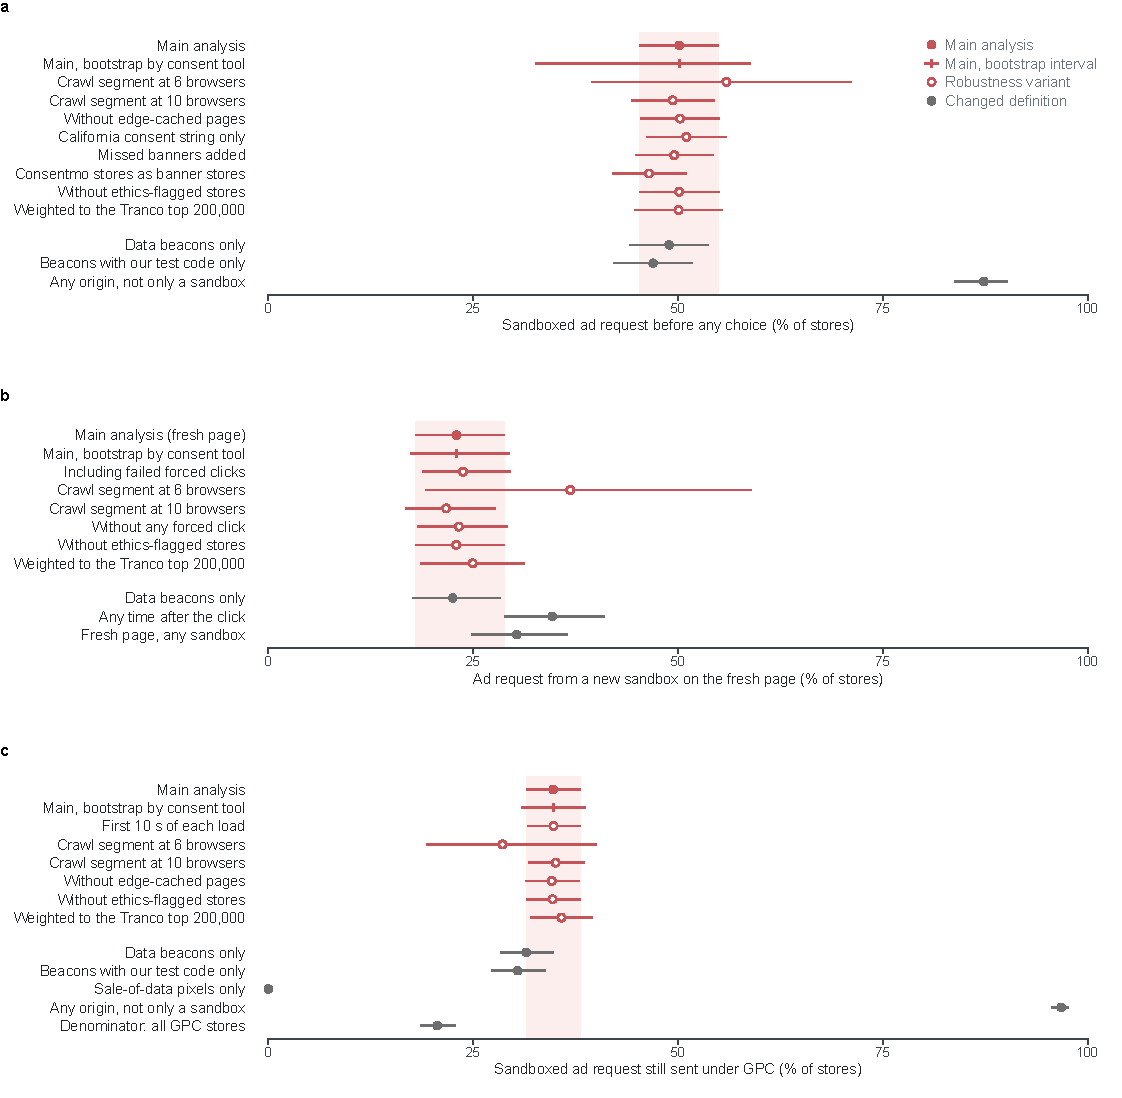
\includegraphics{figS5.pdf}
% GENERATED by paper/integrate_figures_v2.py from figures/v7/supp/caption_supp.tex (v2 figure caption, rendered by the figure script).
% Do not edit: change the figure script and re-run build.sh.
\caption{\textbf{Robustness variants moved the three headline rates little; only changes of definition moved them much.} Each row recomputes one headline rate: (a)~banner stores with a sandboxed ad request before any choice (Default load); (b)~working Decline clicks after which a new sandbox sent an ad request on the fresh page; (c)~stores with a sandboxed ad request under Default that still had one under Global Privacy Control (GPC). Filled brick circle: the main estimate with its Wilson 95\% confidence interval (CI), which the pale brick band carries through the plot (a row whose interval reaches into the band overlaps the main interval; the same band marks these rates in Figs~S2a and S3); `Main, bootstrap by consent tool' is the same main estimate with the bias-corrected and accelerated (BCa) cluster-bootstrap interval in place of the Wilson interval; it is marked by a short vertical brick tick on its interval, not a circle (`Main, bootstrap interval' in the key), because it is not a new estimate, only a wider interval around the same one. Open brick circles: robustness variants (crawl segments at 6 and 10 concurrent browsers; edge-cached pages removed; California consent strings only; the 11 banners the detector missed added; the 54 flagged Consentmo stores counted as banner stores; failed forced clicks included, or all forced clicks removed; the first 10~s of each load; stores flagged in the ethics review removed; design weights with a ratio estimator). Grey circles, set apart below a gap: changed definitions of the measure (data beacons only; beacons carrying our test code; any origin; any time after the click; any sandbox on the next page; pixels declaring sale of data only; all GPC stores as the denominator). Lines: 95\% CIs. The rows, top to bottom, as $k$ of $n$ stores: (a)~main 50.1\% (205 of 409; CI 45.3--54.9\%); BCa interval 32.6--58.9\%; variants 19 of 34; 184 of 373; 203 of 404; 204 of 400; 208 of 420; 215 of 463; 201 of 401; weighted 50.1\%; changed definitions 200 of 409; 192 of 409; 357 of 409. (b)~main 22.9\% (53 of 231; CI 18.0--28.8\%); BCa interval 17.4--29.5\%; variants 57 of 240; 7 of 19; 46 of 212; 53 of 228; 52 of 227; weighted 24.9\%; changed definitions 52 of 231; 80 of 231; 70 of 231. (c)~main 34.7\% (279 of 803; CI 31.5--38.1\%); BCa interval 30.9--38.7\%; variants 279 of 802; 20 of 70; 256 of 730; 276 of 798; 275 of 793; weighted 35.8\%; changed definitions 242 of 769; 229 of 753; 0 of 803; 1,213 of 1,254; 279 of 1,354 (the version of this rate reported in the main text). All 20 robustness variants overlap the main interval, but most are near-complete subsets of the main sample, and the 6-browser segment could detect only differences of about 17--30 percentage points (80\% power).}
\label{fig:s5}

\end{widefig}

\emph{Concurrency segments.} The six-browser segment held 123 stores. Differences between the segments (six minus ten browsers, Newcombe interval) were 6.6 percentage points (95\% CI $-10.6$ to 22.6) for banner stores before any choice (19 of 34 against 184 of 373), 15.1 ($-3.5$ to 37.8) for the fresh-page Decline residual (7 of 19 against 46 of 212), $-6.5$ ($-16.4$ to 5.5) for the GPC residual (20 of 70 against 256 of 730) and 17.7 ($-4.0$ to 28.0) for a first sandboxed request before the banner (17 of 19 against 132 of 184). With 80\% power at the two-sided 5\% level, these comparisons could detect differences of about 25, 28, 17 and 30 percentage points, so the check is underpowered, not confirmatory. The timing outcomes are the ones that CPU contention could shift. In the race, the first third-party marketing sandbox came before a CMP's automatic ``no'' in 13 of 13 loads at six browsers and 129 of 131 at ten, and 45 of 45 and 471 of 481 such sandboxes started before the write.

\emph{Stores excluded for content sensitivity.} After the crawl, a broader title screen found 2 adult-product stores that the sampling screen had missed, and a toy retailer (on its re-check screenshot) and a second store that may be aimed at children were noticed after the crawl (Section~\ref*{M:sec:ethics}). The author excluded these 4 stores from all analyses, so every number in the main article and in this supplement is computed without them; crawl-level counts (planned and failed loads, traffic per store) still include them, because they were loaded.

\emph{Stores flagged in the ethics review.} The retrospective \code{robots.txt} fetch flagged 20 stores (Section~\ref*{M:sec:ethics}): those whose \code{robots.txt} disallowed the exact landing URL we loaded (they include the 2 whose homepage was disallowed). Of these, 17 are analysed main-sample stores (8 showed a banner, 10 sent a sandboxed ad request before any choice, 4 under GPC, none was a blocklist store), 2 are creator stores and 1 was never captured. Table~\ref{tab:s-ethics} recomputes the headline rates, the gate audit and the creator counts without them; no headline rate moves by more than 0.4 percentage points.

\begin{table}[!htbp]
\centering
\caption{Headline rates without the stores flagged in the ethics review ($k/n$, percentage in parentheses). The 4 stores excluded for content sensitivity are excluded from both columns. Pre-choice: a sandboxed ad request before any choice (Default load). Without flagged: the 20 \code{robots.txt}-flagged stores removed (17 main-sample and 2 creator stores had been analysed). Gate: the gate audit of Section~\ref*{M:sec:res-race}. Computed by \code{analysis/analyze.py} (\code{stats.json}, key \code{ethics\_sensitivity}).}
\label{tab:s-ethics}
\footnotesize\setlength{\tabcolsep}{3pt}
\begin{tabular*}{\textwidth}{@{\extracolsep{\fill}}lrr@{}}
\toprule
Measure & All analysed stores & Without flagged \\
\midrule
\tabinput{tables/supp_ethics.tex}
\bottomrule
\end{tabular*}
\end{table}

% ============================================================================
\section{Gate-audit anomalies and edge caches}\label{sec:s-gate}
% ============================================================================

Of 6,983 pixel starts made under a partly denied consent state by pixels that declare a purpose, 97 were for a pixel whose declared purpose was denied at that moment, in 10 loads on 7 stores. In three loads the page came from an edge cache and carried a consent string generated for a visitor in another region. The other seven we cannot explain. In five (S0319\_\_A1, S0552\_\_A1, S1176\_\_A0r, S1176\_\_A2r and S1310\_\_A2), the page's own consent string already declined the purpose and the manager still started the pixel. In two GPC loads (S0301\_\_A2 and S1227\_\_A2), a banner's automatic ``marketing: no'' was dispatched and the first third-party marketing sandbox started 836 and 322~ms later, far beyond the millisecond differences between our clocks (Fig.~\ref*{M:fig:choices}c and Fig.~\ref{fig:s8}d); if the event is dispatched after the write, the starts came later still. The manager may have decided before the write and created the container afterwards, but we did not verify this. The first pages of Decline loads are excluded from the audit because their consent events were not recorded; they hold 140 further flagged starts in 9 loads. As checks of the audit, 0 of 7,458 pixel entries declaring sale of data started under GPC, 2,206 of 2,234 marketing-declaring entries were held back under a denying default, and 8,890 of 8,975 such entries started where marketing was allowed.

Edge caches affect consent more generally. Seven main-sample stores and \storeC served cached pages whose consent string named a region other than our vantage (\storeC: Arizona, in all five loads); on \storeC the cache is a third-party page cache in front of Shopify. In the pilot loads of our unpublished creator-link study, the cached pages of \storeC carried consent strings generated for visitors in the Philippines or Texas, identical with and without the \code{Sec-GPC} header, and the correct state was injected only after Shopify's consent script loaded. Under emulated GPC, TikTok sent requests on 10 of 21 landing loads (9 of 20 per-video landings and the creator-level landing), each time receiving the video code where there was one; in the pilot's Default loads, TikTok's STRICT pixel loaded on 21 of 21 and the Meta library injected by an OPEN pixel on 13 of 21. At the pilot's rate, two misses in a row, as in our GPC and repeat-GPC loads of \storeC, would occur by chance with probability about 0.3 (Fisher's exact test of 9 of 20 against 0 of 2, $p=0.49$), so the rate was not reproduced rather than refuted. Among the 20 loads served from the edge cache, TikTok fired exactly when the WPM created its first worker within about 45~ms of the consent script finishing (10 of 10 such loads) and not otherwise (10 of 10). Because this threshold was chosen after inspecting the same 20 loads, we treat the race as an untested hypothesis (Section~\ref*{M:sec:app-creator}). Excluding edge-cached pages did not change the headline rates (Fig.~\ref{fig:s5}).

% ============================================================================
\section{Outcomes of the pre-crawl predictions}\label{sec:s-predictions}
% ============================================================================

The planned protocol listed eight predictions about the mechanism before the crawl (Section~\ref*{M:sec:method-deviations}). Table~\ref{tab:s-predictions} reports how each fared. Tests of these predictions are confirmatory in the sense that the prediction and its test were fixed before the data were seen; everything else in the main article, including the residual classes, the like-for-like comparison's exclusion of stores whose CMP wrote ``yes'', and the pattern-level match, is exploratory.

\begin{table}[!htbp]
\centering
\caption{The eight predictions written before the crawl, how they were tested, and the result. Numbers are from the main article and this supplement.}
\label{tab:s-predictions}
\footnotesize
\begin{tabularx}{\textwidth}{@{}>{\raggedright\arraybackslash}p{0.27\textwidth}>{\raggedright\arraybackslash}p{0.14\textwidth}>{\raggedright\arraybackslash}X@{}}
\toprule
Prediction & Test & Result \\
\midrule
P1: before any choice, a sandboxed pixel that declares marketing fires where Shopify's region default allows marketing and not where it denies it, whatever the banner or the blocklist says; falsified if a blocklist lowers firing & Gate audit; Figs.~\ref*{M:fig:region-default}a and~\ref*{M:fig:blocked-on-paper}b & Supported. Marketing-declaring entries started in 8,890 of 8,975 cases where marketing was allowed and were held back in 2,206 of 2,234 where it was denied; blocklist stores fired more often than stores without a declaration (difference 13.4 percentage points, 95\% CI 4.0 to 22.8, both samples; main sample alone 13.6 percentage points, 95\% CI $-8.4$ to 35.6). \\
P2: a CMP's blocker never suppresses sandboxed pixel requests (about 100\% of declared-blocked sandboxed pixels fire where the default allows) & Fig.~\ref*{M:fig:situating}b; Fig.~\ref{fig:s7}b--d & Partly supported. No blocker reached a sandbox (on 5 stores it neutralized a vendor's page tag while that vendor's sandboxed pixel sent requests), but configured sandboxed pixels of declared vendors fired for 21 of 29 entries, not all, because Shopify's state held some back. The predicted exception for one tool that hooks worker creation (Transcend) was not tested. \\
P3: a Decline takes effect through Shopify's API from the next page on; pixels started earlier keep sending on the same page & Fig.~\ref*{M:fig:choices}b; Fig.~\ref{fig:s8}b--c & Supported. After a recorded refusal, new sandboxes of pixels declaring a refused purpose fired on 0 of 196 stores; where marketing stayed allowed, 13 of 20 stores still fired; pixels started before the click kept sending on 32 of 196. \\
P4: GPC gates exactly the pixels that declare sale of data & Gate audit; Fig.~\ref*{M:fig:choices}b & Supported. 0 of 7,458 such entries started; under GPC, 279 of 288 stores with a sandboxed pixel not declaring sale of data still fired, against 0 of 515 stores without one. \\
P5: pixels that declare no purpose ignore every choice & Fig.~\ref*{M:fig:choices}b; Fig.~\ref{fig:s8}c & Supported. They kept firing after a recorded refusal on 28 of 196 stores and under GPC on 191 of 1,354. \\
P6: on edge-cached pages, consent outcomes vary between repeat loads; elsewhere repeat loads agree & Repeat loads; \ref{sec:s-gate} & Not supported as stated. Repeat GPC loads agreed on 273 of 273 stores and repeat Default loads on 271 of 273; cached pages carried other regions' consent strings and explain 3 gate-audit loads, but no variation between repeats was seen, and the timing race suggested by the \storeC pilot remains untested. \\
P7: where no consent state can be read, every purpose counts as allowed & Code reading & Not tested dynamically: only 9 of the 1,358 stores returned no consent string. \\
P8: whatever sits in the landing URL reaches every sandboxed pixel that starts & Fig.~\ref*{M:fig:reach}c; Fig.~\ref{fig:s9}a & Supported for the pixels that started: 63.4\% of sandboxed ad beacons carried the full landing URL (TikTok 95.8\%). \\
\bottomrule
\end{tabularx}
\end{table}

% ============================================================================
\section{Detail figures for the main results}\label{sec:s-details}
% ============================================================================

The main figures show one claim each; the detail behind them is collected here. Figure~\ref{fig:s6} gives the per-vendor rates, the timing distribution, the request origins, the per-product strata and the per-store request counts behind Figs.~\ref*{M:fig:situating} and~\ref*{M:fig:region-default} of the main article. Figure~\ref{fig:s7} gives every blocklist subset, all blocklist entries, the re-check tallies and the primary set's entries store by store behind Fig.~\ref*{M:fig:blocked-on-paper}. Figure~\ref{fig:s8} gives the per-vendor and per-subgroup residuals after a choice, the overlapping residual classes by window and the race per load behind Fig.~\ref*{M:fig:choices}. Figure~\ref{fig:s9} gives what reached the vendors by arm, the refusal signals in ad requests, Google's Consent Mode states and the full \storeC timeline behind Fig.~\ref*{M:fig:reach}.

\begin{widefig}
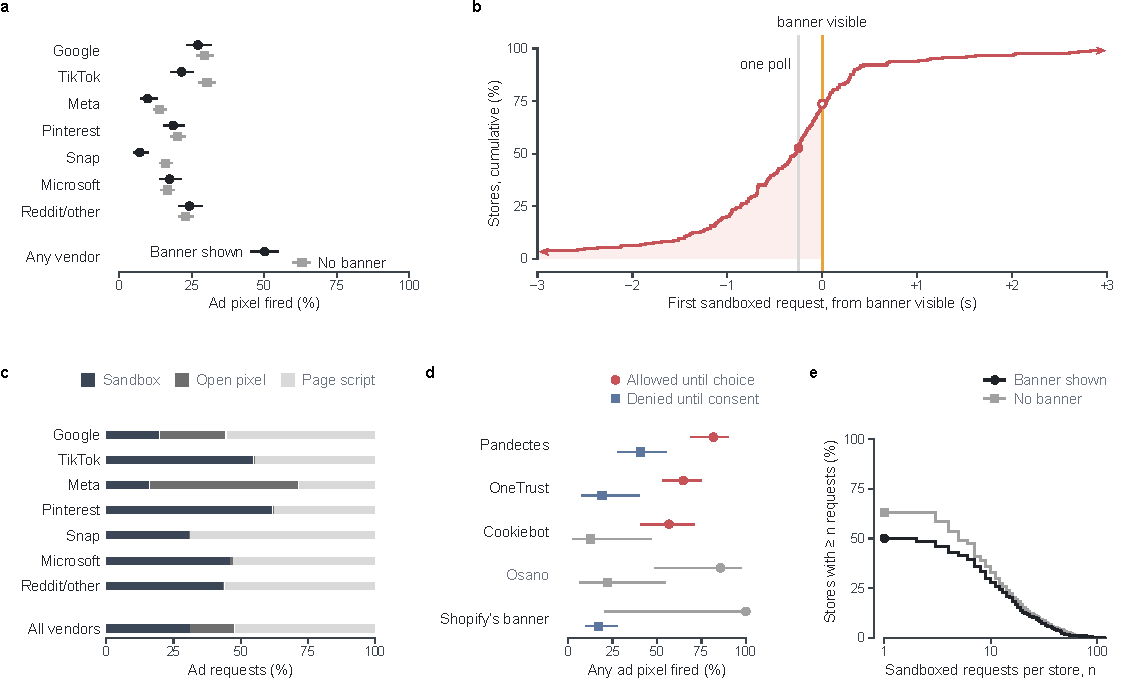
\includegraphics{figS6.pdf}
% GENERATED by paper/integrate_figures_v2.py from figures/v7/supp/caption_supp.tex (v2 figure caption, rendered by the figure script).
% Do not edit: change the figure script and re-run build.sh.
\caption{\textbf{Before any choice, ad pixels of every vendor group fired from Shopify's sandboxes, and most first sandboxed requests came before the banner was visible.} An ad pixel `fired' when a Shopify sandbox sent an ad request before any choice (Default load), as in Figs~3 and 4. Colours, one meaning each: brick, consent lost (the first sandboxed requests in (b); the region default that allows them in (d)); slate, the comparison (d); amber, the banner becoming visible; dark slate, Shopify's sandbox (c); black and grey, stores with and without a banner (a, e), a contrast that is not about consent; other greys, context. (a)~Stores on which an ad pixel of each vendor group fired, among the 409 stores that showed a banner (black circles) and the 949 that did not (grey squares), each named on the `Any vendor' row, which is set apart below. Horizontal lines in (a) and (d): Wilson 95\% confidence intervals (CIs), in the colour of their mark. Keys in (c) to (e) sit above their plots. (b)~The 205 banner stores with a pre-choice sandboxed request: cumulative share whose first sandboxed ad request had been sent by time $t$, timed from the banner becoming visible (amber line; the time axis of Fig.~1b,c); thin light grey line: one polling interval of the banner detector (250~ms) before the banner. The pale brick ground under the curve, left of the amber line, marks the stores that sent before the banner: the open ring where the curve meets the amber line is 151 of 205 stores (73.7\%), and the dot on the light grey line the 108 (52.7\%) that sent more than one poll before it. The 9 stores whose first request lies beyond the axis are counted at its ends, so the curve starts above the bottom of the axis and ends below its top; where it leaves the axis it ends in an arrowhead. In the 46 such stores loaded twice, `request first' agreed in 36 ($\kappa$ 0.54). (c)~Origin of all ad requests in the Default load, by vendor group: Shopify sandbox (dark slate, the colour of the sandbox frame in Fig.~1a; web worker or sandboxed iframe, including frames nested in it), Shopify's open pixel (pixel type `OPEN', which runs in the page; mid grey) and ordinary page scripts and frames (light grey); thin white gaps separate the segments. Requests relayed from a sandbox by Shopify code in the page are Google's only (115 of 20,503; 0.6\%): they keep their share of the bar but are narrower than a segment gap and are not drawn. Sandboxed share of each group's ad requests: Google 20.1\% (4,112 of 20,503), TikTok 55.1\% (2,280 of 4,135), Meta 16.5\% (408 of 2,478), Pinterest 62.2\% (1,189 of 1,911), Snap 31.0\% (612 of 1,973), Microsoft 46.3\% (1,093 of 2,363) and Reddit/other 43.7\% (2,910 of 6,653); across all vendors 31.5\% (store-bootstrap 95\% CI 29.8--33.2) of 40,016 requests were sandboxed. (d)~Banner stores on which any ad pixel fired, within five consent products, by Shopify's region default: `allowed until choice' (brick circles) and `denied until consent' (slate squares). These are the shares of Fig.~3a's four product rows, plus Shopify's banner, which Fig.~3a lists in its caption but does not draw, here under Fig.~3a's axis title with the stores under each default: Pandectes 49 and 44; OneTrust 68 and 21; Cookiebot 37 and 8; Osano 7 and 9; Shopify's banner 1 and 65; grey marks: fewer than 10 stores under one default (Cookiebot `denied until consent', both of Osano's, whose name is grey, and Shopify's banner `allowed until choice'). The pooled Mantel--Haenszel difference over 12 products is in Fig.~3a (right). (e)~How many sandboxed ad requests each store sent before any choice (Default load, no click): share of stores with at least $n$ requests (complementary cumulative distribution; logarithmic $n$ axis), for the stores that showed a consent banner (black) and those that showed none (grey). Marks at the left end, at least one request: 205 of 409 banner stores and 598 of 949 stores without a banner; Wilson 95\% CIs 45.3--54.9\% and 59.9--66.0\%; a cluster bootstrap by consent tool widens them to 32.6--58.9\% and 56.8--68.0\%.}
\label{fig:s6}

\end{widefig}

\begin{widefig}
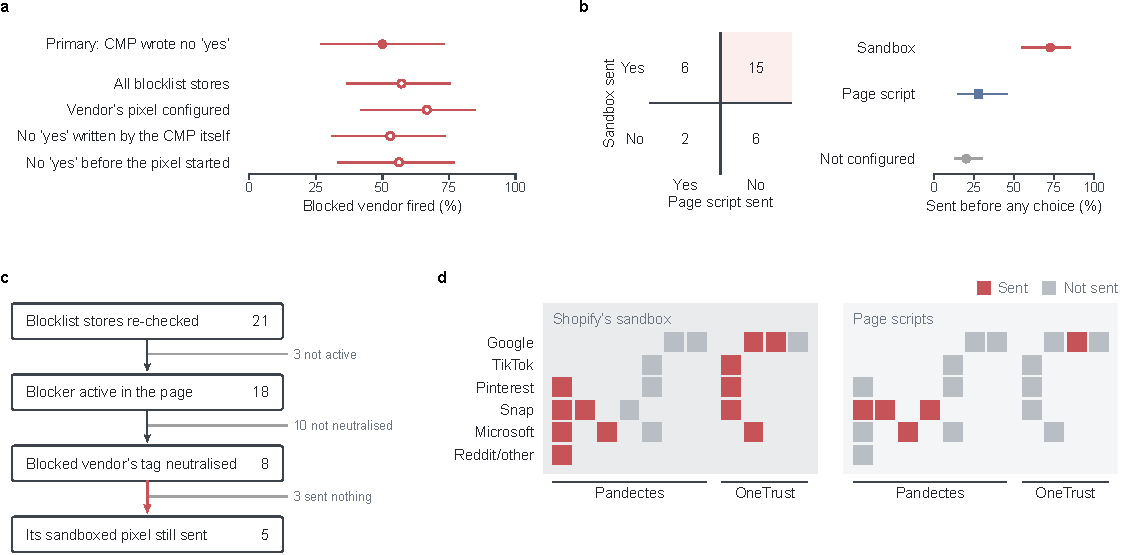
\includegraphics{figS7.pdf}
% GENERATED by paper/integrate_figures_v2.py from figures/v7/supp/caption_supp.tex (v2 figure caption, rendered by the figure script).
% Do not edit: change the figure script and re-run build.sh.
\caption{\textbf{Blocked on paper in the main sample: vendors that a blocklist named still fired from Shopify's sandbox in every subset, while the blocker acted only on the page.} Colours: brick, sent before any choice (consent lost); slate, the comparison route (a page script); greys, context. All counts are for the main sample (Tranco top 200,000 ranks); the expansion to ranks 200k--1M and the combined estimate (primary set: 46 of 89 stores) are in Fig.~4a. (a)~Blocklist stores on which the vendor that the consent-management platform's (CMP's) blocklist declared blocked fired: its own sandboxed Shopify pixel sent an ad request before any choice (Default load). Top, set apart, the primary estimate (filled brick circle): stores whose CMP wrote no `marketing: yes', 50.0\% (7 of 14). Below, the sensitivity subsets (open brick circles): all 21 blocklist stores (12 fired); the stores with the vendor's sandboxed pixel configured (10 of 15); without the 4 stores whose CMP wrote `yes' by itself (2 of them because Pandectes' bot rule detected our automated browser; 9 of 17); and without the 5 stores with a `yes' before the pixel started (9 of 16). Horizontal lines: Wilson 95\% confidence intervals (CIs). (b)~The blocklist entries on the 21 blocklist stores. Left: the 29 entries whose vendor has a configured sandboxed Shopify pixel (15 stores) as a 2~$\times$~2 matrix of counts: whether the vendor sent an ad request before any choice from Shopify's sandbox (rows) and, counted independently, from an ordinary page script (columns); both routes 6; the sandbox only 15 (pale brick cell: consent lost only through the sandbox; the cells are split by two crossing rules, as in Fig.~S4a--c); a page script only 2; neither 6. Right: share of entries sent before any choice, with Wilson 95\% CIs: the same entries from the sandbox (brick circle; 21 of 29) and from a page script (slate square; 8 of 29) and, set apart, the 75 entries without an identified configured sandboxed pixel (20 stores; classic tag, open pixel or unknown installation) by any route (grey circle; 15 of 75). (c)~One re-check load per blocklist store, after the main crawl, drawn as the ledger of Fig.~2a (each box: the stage, left, and its number of stores, right; the stores that leave a stage branch right, with their reason in grey, so that each count is the one above minus its branch; the brick arrow marks the leak). Of the 21 blocklist stores the blocker was active in 18; on 8 it neutralised the tag of a vendor it declared blocked; on 5 of these that vendor's sandboxed pixel still sent an ad request. (d)~The primary set store by store: its 19 blocklist entries whose vendor has a configured sandboxed Shopify pixel, on 11 stores, as two store $\times$ vendor-group matrices with one layout, each on the ground of its region in Fig.~1a. Left, on the darker grey ground of the pixel sandboxes: the route through Shopify's sandbox (12 of 19 entries sent an ad request before any choice); right, on the light grey ground of the page: the route through an ordinary page script (5 of 19). Columns are the stores, grouped by the consent tool whose blocklist declared the vendor blocked (named below a rule under its columns); rows are the vendor groups used in every other figure (the one Reddit/other entry is Amazon Ads); brick: sent by that route; grey: not sent by that route (key above the right matrix); blank: no entry. The same position in both matrices is the same entry: 4 entries were sent by both routes and 6 by neither. Blocklists are readable for Pandectes, OneTrust and Cookiebot only.}
\label{fig:s7}

\end{widefig}

\begin{widefig}
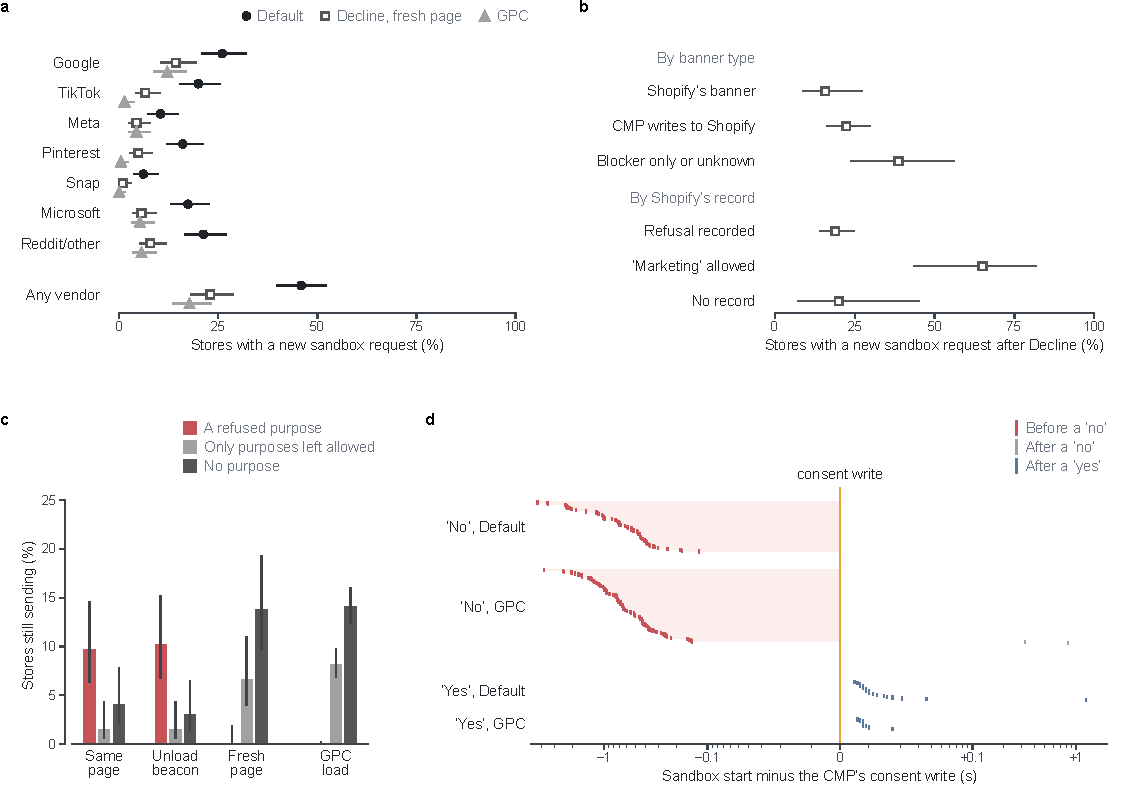
\includegraphics{figS8.pdf}
% GENERATED by paper/integrate_figures_v2.py from figures/v7/supp/caption_supp.tex (v2 figure caption, rendered by the figure script).
% Do not edit: change the figure script and re-run build.sh.
\caption{\textbf{After a choice, new sandboxes kept sending ad requests, and where a consent tool wrote `no' without a click a sandbox had almost always started first.} Colours: brick, consent lost; slate, the comparison; amber, the consent tool's write; greys, context. Every key sits above its plot. (a)~The per-vendor estimates of Fig.~5a, repeated here (they are not new estimates) as rows on the scale of (b), so that the vendors can be read against the subgroups of (b): on the 231 stores where the Decline click worked, stores on which a new sandbox sent an ad request to each vendor group under Default (filled black circles), on the fresh page after Decline (open squares; new sandboxes, 10~s) and under Global Privacy Control (GPC; filled grey triangles; first 10~s); `Any vendor' is set apart below. Lines in (a) and (b): Wilson 95\% confidence intervals (CIs), in the colour of their mark. (b)~The fresh-page measure of (a), any vendor (open squares), by banner type (top three rows; each grouping is named in grey above its rows): Shopify's own banner 9 of 57; a consent-management platform (CMP) that writes to Shopify 32 of 143; a blocker only, unknown or none 12 of 31; and by the state Shopify recorded after the click (bottom three rows): explicit refusal 37 of 196; `marketing' still allowed 13 of 20; no record 3 of 15. (c)~What the pixels that still sent requests declare, by window after a Decline (same page after the click; unload beacon at the reload; fresh page) among the 196 stores where Shopify recorded a refusal, and under GPC among the 1,354 stores where Shopify set `sale of data: no'. Share of the window's stores whose still-sending pixel declares a purpose the visitor refused (brick), only purposes the choice left allowed (grey) or no purpose (dark grey), in the class names, colours, key order and bar form of Fig.~5b: one thin bar per class from zero, side by side rather than stacked because a store can be in several classes, with its Wilson 95\% CI as a dark line, as in Fig.~5b; a class with no store has no bar, only its interval. Stores whose pixel declares a refused purpose: 19 (same page), 20 (unload beacon), 0 (fresh page) and 0 (GPC); only purposes left allowed: 3 (same page), 3 (unload beacon), 13 (fresh page) and 111 (GPC); no purpose: 8 (same page), 6 (unload beacon), 27 (fresh page) and 191 (GPC). A store can appear in several classes and windows (one class per store: Fig.~5b). (d)~The race in Fig.~5c's raster and time axis: one row per page load in which a CMP wrote `marketing: no' or `yes' without a click, in four blocks (`no' in the Default load, 59 loads; `no' under GPC, 87; `yes' in the Default load, 22; `yes' under GPC, 13), each block sorted by its loads' first third-party sandbox that declares `marketing'. One tick per load, at that sandbox's start minus the CMP's consent write (amber line, named above the plot), on Fig.~5c's symmetric-log axis (linear close to the write, logarithmic beyond; the two innermost tick labels of Fig.~5c are omitted here). Brick: the sandbox started before the `no'; grey: after the `no'; slate: after a `yes'. A wider gap sets the two `yes' blocks apart from the two `no' blocks. The pale brick ground between the brick ticks and the amber line marks the time each of those sandboxes ran before the `no'. In 144 of 146 `no' loads a sandbox started first (the other 2 are GPC loads); in all 35 `yes' loads it started after. Stores where a CMP wrote `marketing: no' without a click and a sandboxed ad request was still sent before any choice: 39 of 65 (60.0\%; Wilson 95\% CI 47.9--71.0\%). The per-sandbox version is Fig.~5c.}
\label{fig:s8}

\end{widefig}

\begin{widefig}
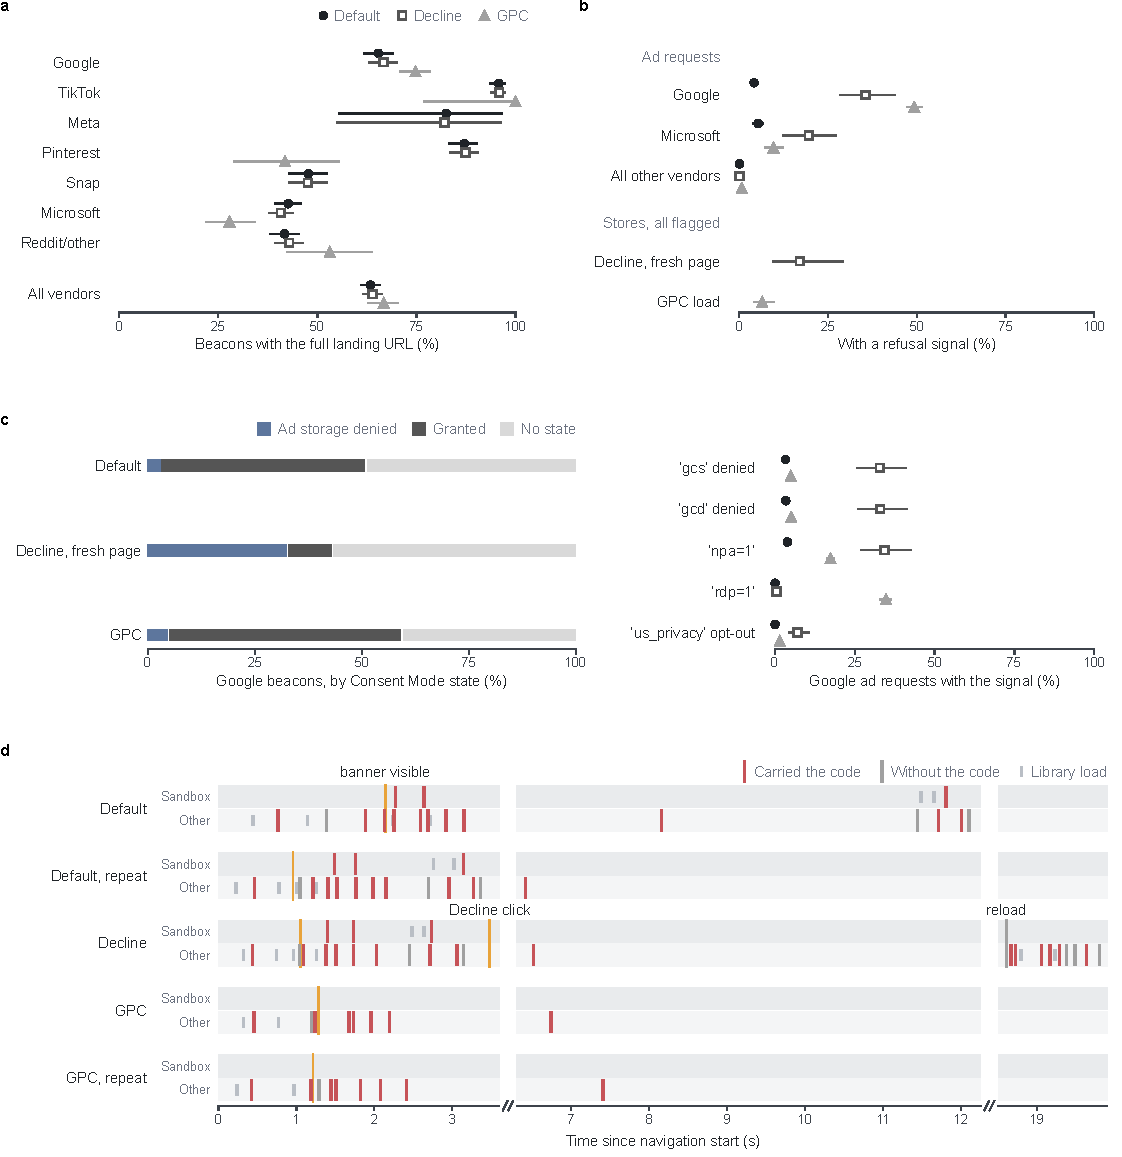
\includegraphics{figS9.pdf}
% GENERATED by paper/integrate_figures_v2.py from figures/v7/supp/caption_supp.tex (v2 figure caption, rendered by the figure script).
% Do not edit: change the figure script and re-run build.sh.
\caption{\textbf{Vendors received the full landing URL in every load, refusal signals mostly in Google's requests, and a creator's per-video code on every load of Store C.} Colours: brick, requests that carried the per-video code; slate, Google beacons whose Consent Mode state denied ad storage; amber, the banner becoming visible and the Decline click; greys, context. (a)~Sandboxed ad beacons carrying the full landing URL with our test code, by vendor group and load: Default (filled black circles), Decline (open squares) and Global Privacy Control (GPC; filled grey triangles); key above the plot; Korn--Graubard 95\% confidence intervals (CIs) clustered by store. Stores per load (Default / Decline / GPC): Google 390 / 393 / 172; TikTok 346 / 344 / 16; Meta 18 / 18 / 4; Pinterest 264 / 264 / 14; Snap 179 / 178 / 6; Microsoft 226 / 224 / 64; Reddit/other 314 / 309 / 84; all vendors 769 / 764 / 242. A load with fewer than 10 stores for a vendor (Meta and Snap under GPC) is not drawn. Markers in (b) and (c) as in (a). (b)~One plot on the scale of (a), in two groupings named in grey above their rows. `Ad requests': ad requests carrying a refusal signal in the URL (Google: Consent Mode, `npa', `rdp' or `us\_privacy'; Microsoft: `asc=D'), in the Default load, on the next page after Decline and in the GPC load; 95\% CIs from resampling stores (percentile bootstrap, 2,000 resamples). On the fresh page after Decline (open squares): Google 434 of 1,220 (35.6\%), Microsoft 80 of 408 (19.6\%), all other vendors 0 of 1,211. `Stores, all flagged': stores still sending sandboxed ad requests on which every one of them carried a refusal signal (open square: the fresh page after Decline; grey triangle: GPC): 9 of 53 on the fresh page after Decline and 18 of 279 under GPC (Wilson 95\% CIs). (c)~Google's ad requests only. Left: beacons by the Consent Mode state in their `gcs' parameter: ad storage denied (G100 or G101; slate), granted (G111; dark grey) or no state (light grey); thin white gaps separate the segments; key above the plot. Beacons: 20,480 in the Default load, 1,219 on the fresh page after Decline and 16,703 in the GPC load; other states (at most 0.3\% of a load's beacons) are too few to draw. Right: share of Google's ad requests carrying each signal (`gcs' or `gcd' with ad storage denied, `npa=1', `rdp=1', a `us\_privacy' opt-out; markers as in (a)). These are request-level shares of the same requests (Default 20,503; Decline 1,220; GPC 16,718); because requests cluster within stores, their 95\% CIs come from resampling stores, as in (b); an interval narrower than its marker is hidden behind it. (d)~Store~C, a creator-linked store, reached from the creator's video link: every ad request in five loads (Default and its repeat, Decline, GPC and its repeat) as an event strip on one broken time axis with one scale. The axis is cut (double slashes) where nothing was sent or happened for a long span, and two short, sparse stretches share the middle stretch. Each load has a lane of requests from a sandbox (`Sandbox', on the darker grey ground of Fig.~1a's pixel sandboxes) and a lane of all others (`Other', on the light grey ground of the page). One tick per group of requests of one vendor group and kind less than 50~ms apart, at their mid time (37 ticks stand for more than one request); tall ticks: data beacons and other requests, brick when at least one request of the tick carried the per-video code and grey when none did; short light grey ticks: library loads, none of which carried the code (key above the plot). Amber lines: the banner becoming visible and the Decline click; grey line: the reload in the Decline load; each event is named above its own line, the banner once. In the sandbox lanes of the Default, repeat and Decline loads the first two ticks are Google's, the two short light grey ticks are TikTok's library loads and the last tick stands for the 4 code-carrying TikTok requests counted in the caption of Fig.~6a; nothing was sent from a sandbox in the GPC loads. The code reached 5 vendors (3 other than Google) in the Default load and 5 (3) in its repeat; in the Decline load 5 before the click and 4 after the reload (0 from a sandbox); under GPC 3 (1) and 3 (1) in its repeat. Signals carried in request bodies are not visible.}
\label{fig:s9}

\end{widefig}


% ============================================================================
\section{Round 4: blocklist expansion and pilot beyond Shopify}\label{sec:s-r4}
% ============================================================================

The Round 4 crawl ran on 27 September 2026 with the crawler of the main study, unchanged apart from its plan and output paths, the Default, Decline and GPC arms, at most six concurrent browsers, at least 10~s between two loads of a site and a \code{robots.txt} check before the first load (Section~\ref*{M:sec:method-r4} of the main article). Its numbers are generated by a separate pipeline whose outputs are merged unchanged into the analysis outputs of the main study and checked by the same number trace.

\emph{Expansion sample.} Tranco ranks 200,001--1,000,000 of list L5PZ4 were resolved with the main sample's DNS rule, and the flagged domains were screened in a seeded random order with one homepage request each. In the drawn prefix of 12,015 flagged domains, 11,354 storefronts were eligible under the main sample's rules, 1,252 ran Pandectes, OneTrust or Cookiebot, and 215 published a readable blocklist that named an ad vendor. Of these, 98 declared the vendor blocked before any choice for a California visitor, 95 declared the opposite and are not part of the stratum, and 22 could only be settled at run time; the 120 stores of the first and last groups were all loaded. The screen stopped short of its target of 250 stores, so the stratum is every eligible store in a random prefix, not a sample of fixed size. Of the 120 stores, 116 were captured in all three arms, and the blocklist was in force at run time on 96 (93 Pandectes, 3 OneTrust). The static screen had predicted a blocklist before any choice on 95 of the 116, and it was in force on 93 of these; it was in force on 3 of the 21 that could only be settled at run time. The blocked-on-paper estimands were computed by the main pipeline's own code; on the main sample it reproduced all 13 compared estimands exactly.

\emph{Blocked-on-paper results by sample.} On 21 of the 96 expansion stores the CMP wrote ``marketing: yes'' without a click, and the declared vendor fired from the sandbox on 55 of all 96 (57.3\%, 47.3--66.7\%) and on 39 of the other 75 (52.0\%, 40.9--62.9\%). Among these 75, the vendor fired on 36 of the 52 whose region default allowed marketing and on 3 of the 23 whose default denied it, and any sandboxed ad pixel fired on 51 (68.0\%, 56.8--77.5\%). Within the expansion alone, the like-for-like difference against the main sample's reference was 13.3 percentage points (95\% CI 3.4 to 23.3) among stores whose CMP wrote no ``yes''. Pooled over both samples, the primary rate by region default was 42 of 59 where the default allowed marketing and 4 of 30 where it denied it. At the level of entries, counting every declared-blocked ad vendor of a primary store whether or not a sandboxed pixel of it was configured, 15 of 74 entries fired in the main sample and 70 of 292 in the expansion (24.0\%, 17.6--31.4\%, clustered by store). The design-weighted primary rate over both samples is 51.8\% (40.6--62.2\%).

\emph{Pilot beyond Shopify.} Figure~\ref{fig:s10} shows the per-setup rates. Of the 195 selected sites, 190 were loaded; 5 were skipped because their \code{robots.txt} could not be retrieved, and on 4 only the address without our canary was allowed. On Wix, 26 sites' own consent policy denied advertising to our visitor, and 16 of them sent an ad request (61.5\%, 42.5--77.6\%); on 53 whose policy allowed it, 23 did (43.4\%, 31.0--56.7\%). On BigCommerce, stores with the platform's consent tracking enabled sent an ad request before any choice on 33 of 56 (58.9\%, 45.9--70.8\%), those without it on 19 of 21. Worker code saw \code{navigator.globalPrivacyControl} as true in 82 of 85 Wix workers under GPC. Google's two consent parameters, \code{gcs} and \code{gcd}, agreed on all 1,655 first-party and third-party hits that carried both. On the Partytown sites the Partytown configuration was read at run time on 4 of the 5 captured sites, and none of its workers sent any request in any arm; the one Zaraz site made no Zaraz track call in any arm and showed no banner.

\begin{widefig}
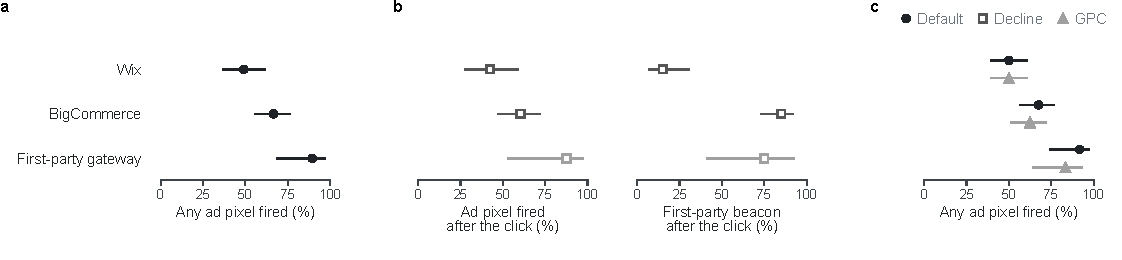
\includegraphics{figS10.pdf}
% GENERATED by paper/integrate_figures_v2.py from figures/v7/supp/caption_supp.tex (v2 figure caption, rendered by the figure script).
% Do not edit: change the figure script and re-run build.sh.
\caption{\textbf{Beyond Shopify: in a pilot of selected Wix, BigCommerce and first-party-gateway sites, ad requests were common before any choice, after a working Decline and under Global Privacy Control (GPC).} The sites are a pilot of selected sites, not a sample: 80 Wix and 80 BigCommerce sites (80 and 77 captured) and 26 sites whose Google tag loads through a first-party tag gateway or tagging server (`first-party gateway'; 24 captured). They were crawled on 27 Sep 2026 from one California vantage point with the same three loads as the main study (Default, Decline, GPC). An ad pixel `fired' when the site sent an ad request: a request to an advertising vendor, or a first-party request whose wire format names Google Ads, Meta or TikTok (the axis titles of Figs~3 and 4). Forwarding onward from a server (server-side) is not observable and is never inferred. The three setups are the rows of every plot. (a)~Banner sites on which any ad pixel fired in the Default load, before any choice: Wix 28 of 57; BigCommerce 48 of 72; first-party gateway 17 of 19. (b)~Sites where the Decline click worked. Left: an ad pixel fired after the click, on the same page or the next page (Wix 14 of 33; BigCommerce 32 of 53; gateway 7 of 8). Right: a first-party collect beacon after the click, that is a GA4, Google Ads, Universal Analytics, Meta or TikTok beacon sent to the site's own domain or tagging server: Wix 5 of 33; BigCommerce 45 of 53; gateway 6 of 8. (c)~All sites with a Default and a GPC load: any ad pixel fired in each load, Default above GPC (Wix 40 and 40 of 80; BigCommerce 52 and 48 of 77; gateway 22 and 20 of 24). Markers, in one key above (c): Default load (filled black circle), Decline load (open square), GPC load (filled grey triangle); lines: Wilson 95\% confidence intervals; light grey marks: fewer than 10 sites (the gateway sites with a working Decline click, in (b)); every plot has the same scale. Two case studies give no rates and are not drawn. Partytown, which runs third-party scripts in a web worker: of 8 selected sites, 5 were captured; requests from Partytown workers numbered 0 in all loads, and the 3 sites with an ad request in the Default load sent it from the top frame's main thread (3 sites) and from iframes (1 site). Zaraz, which runs tools on Cloudflare's servers: on the 1 selected site Zaraz loaded, made 0 track calls in all loads, and sent no ad request in any load. Rates describe the selected sites only: they are not population estimates, the setups are not compared statistically, and they are not comparable with the Shopify rates of the main study, which count ad requests from Shopify's sandbox.}
\label{fig:s10}

\end{widefig}

% ============================================================================
\section{Further methods, results and discussion}\label{sec:s-extended}
% ============================================================================
% Added 2026-09-28 for the Computers & Security length target: text moved here from the main article, numbers unchanged.

This note holds detail that was moved out of the main article to keep it within the journal's usual length. Each paragraph names the section of the main article that it extends. References to the literature are given in the main article.

\subsection*{Methodology (Section~\ref*{M:sec:method})}

\emph{Content screen (Section~\ref*{M:sec:method-sample}).} The 21 titles flagged by a keyword screen for adult or child-directed content were reviewed without an independent human rater (Section~\ref*{M:sec:method-ai}). A broader screen after the crawl found 2 adult-product stores that the keyword screen had missed; they and two possibly child-directed stores were excluded from all analyses (Section~\ref*{M:sec:ethics} and \ref{sec:s-sens}). The landing page was the store's first product link, which need not be a typical product (\ref{sec:s-sample}).

\emph{Decline arm (Section~\ref*{M:sec:method-arms}).} Reject controls were matched by text (``Decline'', ``Reject all'' and equivalents in several languages) or CMP-specific selectors; Accept, settings and ``Do not sell'' links were never clicked, and banners without a first-layer reject control were not clicked. The 9 failed forced clicks are reported separately (\ref{sec:s-audit}).

\emph{Attribution (Section~\ref*{M:sec:method-attr}).} A sandboxed request is \emph{relayed by Shopify} only when its initiator stack holds nothing but Shopify or store scripts. The seven vendor groups are Google, TikTok, Meta, Pinterest, Snap, Microsoft, and Reddit and others. CORS preflights, which DevTools reports in the page's session, are not counted. Vendor refusal signals include Google Consent Mode values and the \code{npa}, \code{rdp} and \code{us\_privacy} parameters.

\emph{Outcomes (Section~\ref*{M:sec:method-outcomes}).} Store-level rates before any choice use the Default load; the Decline load before the click enters only the comparison of whole visits (Section~\ref*{M:sec:res-gpc}). After Decline, any sandboxed request after the click is a secondary outcome.

\emph{Statistical analysis (Section~\ref*{M:sec:method-stats}).} The Wilson intervals treat the sampled stores as a draw from a super-population without a finite-population correction; because the three upper buckets are censuses, corrected intervals for the frame would be narrower (14.0--17.3\% instead of 13.5--17.8\% for the projection in Section~\ref*{M:sec:app-projection}), so the reported intervals are conservative for sampling error within the frame, and none includes the frame's coverage error. The BCa cluster bootstrap by consent tool uses 2,000 resamples. Shares whose unit is a request, a pixel entry, a pixel start or a store--vendor pair, and Cohen's $\kappa$, have intervals that resample stores (a percentile bootstrap, or the Korn--Graubard interval where marked); we read $\kappa \ge 0.81$ as almost perfect agreement. Population estimates use the design weights and propagate the uncertainty of the frame size; cells with fewer than five stores are not interpreted.

\emph{Round 4 (Section~\ref*{M:sec:method-r4}).} The crawl ran on 27 September 2026 between 19:56 and 20:57~UTC with the crawler unchanged apart from its plan and output paths. In the expansion screen, the blocklist was in force at run time on 93 of the 95 stores for which the static screen had predicted it, and on 3 of the other 21; the screen did not reach its target of 250 stores within the time available, so the 120 are all stratum stores in a random prefix of 12,015 flagged domains (\ref{sec:s-r4}). The like-for-like reference stayed the main sample's banner stores without a readable declaration. In the pilot, first-party requests were attributed to a vendor only when their wire format named it (for example Google Ads' \code{/ccm/collect} path or Meta's \code{/tr?id=} beacon); rates carry Wilson intervals and a site bootstrap, and Partytown and Zaraz are reported as case studies.

\emph{Changes to the planned protocol (Section~\ref*{M:sec:method-deviations}).} The planned protocol and eight predictions were written in an internal note before the crawl; Table~\ref{tab:s-predictions} reports how each fared, which separates the confirmatory from the exploratory results. Three changes were made during the crawl. (i) The plan set a limit of about six concurrent browsers. On 26 September 2026 at 07:35~UTC, after the first 578 loads, a process started by another automated session of the project (a coordinating session, not the crawl session) stopped the crawler and restarted it with the same code, plan and seed at ten concurrent browsers; its log note says this was at the user's request, which the crawl session could not verify. The other 4,398 loads ran at ten browsers and the 19 retries at six. We report it as a deviation. We kept these loads because per-site pacing was unchanged (at least 10~s between two loads of a store). The six-browser segment is small, so comparing the segments could detect only differences of about 17--30 percentage points (\ref{sec:s-sens}); the check is underpowered, not confirmatory. (ii) A first banner detector counted an invisible full-screen wrapper of one CMP (Consentmo) as a banner; the 510 loads it had judged were re-run with the final detector. (iii) The next-page reload of the Decline arm was added (257 page loads). After an internal audit and all other analyses, three checks that the plan did not contain were added: the re-check crawl, a retrospective fetch of each store's \code{robots.txt} (Section~\ref*{M:sec:ethics}) and a check of the frame's recall (Section~\ref*{M:sec:method-sample}); their results are reported as they came out.

\subsection*{Results (Section~\ref*{M:sec:results})}

\emph{Before any choice (Section~\ref*{M:sec:res-prechoice}).} Neither library loads nor missed banners explain the pre-choice rate on banner stores: counting data beacons only gave 200 of 409 (Fig.~\ref{fig:s5}), and adding the 11 banners that the detector missed (\ref{sec:s-audit}) gives 208 of 420 (49.5\%). Of the ad requests in Default loads, the sandbox carried most for Pinterest (62\%) and TikTok (55\%), whose app pixels run in STRICT workers, and least for Google (20\%) and Meta (16\%), whose apps run as OPEN pixels (Table~\ref{tab:s-vendor}).

\emph{Blocked on paper (Section~\ref*{M:sec:res-paper}).} Weighting each sample by its design gives 51.8\% (40.6--62.2\%). In the main sample, the vendor fired on 10 of the 15 stores with a configured sandboxed pixel of a declared vendor (66.7\%, 41.7--84.8\%), and two further exclusion rules, chosen after the data were seen, give 9 of 17 and 9 of 16 (\ref{sec:s-cmp}). Where a banner store's Shopify configuration listed a vendor group's sandboxed pixel (764 store--vendor pairs on 318 stores), that pixel fired before any choice in 391 pairs (51.2\%, 45.4--57.0\%, clustered by store; Fig.~\ref{fig:s2}b); the rates per consent tool mostly track the region default and describe the stores that use each product, not its quality (Table~\ref{tab:s-cmp}). Counting every declared-blocked ad-vendor entry of the primary stores in both samples, whether or not a sandboxed pixel of that vendor was configured, 85 of 366 fired from the sandbox (23.2\%, 17.2--30.1\%, clustered by store); because we never clicked Accept, entries that sent nothing cannot be classified as blocked or not installed.

\emph{Decline (Section~\ref*{M:sec:res-decline}).} The fresh-page residual was 9 of 57 stores (15.8\%) with Shopify's own banner, 32 of 143 (22.4\%) with CMPs that write to Shopify, and 12 of 31 (38.7\%) with blocker-only or unknown tools (Fig.~\ref{fig:s8}b); exploratory models, which cannot separate product from region default, found no clear difference after adjustment (\ref{sec:s-models}).

\emph{GPC (Section~\ref*{M:sec:res-gpc}).} Across all origins, ad requests continued under GPC on 1,213 of the 1,254 stores that had any under Default, most to Google, whose app declares no purpose to Shopify. For persistence after the choice, the reduction from Default was 28.1 points (95\% CI 22.2 to 33.9) against GPC's advantage over a working Decline of 5.2 points. Counting Decline attempted rather than Decline that worked, which adds the 9 failed forced clicks, gives 57 and 42 of 240 stores (difference 6.2 percentage points, 95\% CI 1.3 to 11.3).

\emph{Beyond Shopify (Section~\ref*{M:sec:res-beyond}).} Before any choice, an ad request left the page on 28 of 57 Wix sites that showed a banner (49.1\%, 36.6--61.7\%), on 48 of 72 BigCommerce sites (66.7\%, 55.2--76.5\%) and on 17 of 19 gateway sites (89.5\%, 68.6--97.1\%). On BigCommerce, first-party collection and a server-set identifier cookie each followed 45 of the 53 refusals (84.9\%). GPC made little difference: ad requests occurred on 40 of 80 Wix sites under both Default and GPC, and on 48 of 77 BigCommerce sites under GPC against 52 under Default. Where Wix's own consent policy denied advertising to our visitor, 16 of 26 sites still sent an ad request, 15 of them from the top frame, so here too the platform's policy did not govern every tag. On the 5 captured Partytown sites no request came from a Partytown worker, and the ad requests on 3 of them came from the top frame's main thread or from iframes; the one Zaraz site loaded Zaraz and sent no tracking request.

\subsection*{Reach and robustness (Section~\ref*{M:sec:application})}

\emph{Refusal signals (Section~\ref*{M:sec:app-url}).} A flagged request, still sent but asking the vendor to restrict its use of the data, is not counted as under-declaration.

\emph{\storeC (Section~\ref*{M:sec:app-creator}).} After the Decline and the reload the creator's code reached 4 other vendors, none from a sandbox, and under GPC it reached two Google services, whose app declares no purpose, and tvScientific, from a main-thread script. Every \storeC load received an edge-cached consent string generated for a visitor in Arizona, the case that Shopify fix (iv) in Section~\ref*{M:sec:disc-fix} addresses; pilot loads of an earlier, unpublished study of this store are compared with ours in \ref{sec:s-gate}.

\emph{Stability and GPC injection (Section~\ref*{M:sec:app-validation}).} Per-store request counts repeated: among stores with sandboxed requests in both loads, Spearman's $\rho$ was 0.972 (0.916--1.000; 161 stores) for Default and 0.900 (0.695--1.000; 50 stores) for GPC. The injected flag read true in all 2,735 LAX iframes and 848 other workers of the GPC arm, and preceded the worker's own code in all 4,720 STRICT workers; the agreement between Brave's native GPC and our emulation includes the 39 stores and 109 pairs on which Default and GPC differed.

\emph{Automation.} The page probe also read \code{navigator.webdriver} as true in all 127 usable re-check loads. The signature of Pandectes' bot setting is a banner configured visible, a banner element present but hidden, and a ``yes'' without a click. A rule that hides the banner from bots lowers the banner count.

\emph{Sensitivity.} The robustness variants include excluding edge-cached pages or the flagged stores, and the design weights. The six-browser crawl segment differed from the ten-browser segment by 6.6 percentage points (95\% CI $-10.6$ to 22.6) for banner stores before any choice and by 17.7 ($-4.0$ to 28.0) for a first request before the banner; with 123 stores it could detect only differences of about 17--30 points (\ref{sec:s-sens}). The 12 forced clicks agreed with the rule for a working click (\ref{sec:s-audit}).

\emph{Projection (Section~\ref*{M:sec:app-projection}).} The projections treat the 38 sampled stores that were not captured as missing at random within their rank bucket. The frame's recall is 23\% in the top bucket, and it excludes storefronts on \code{shop.} and \code{store.} subdomains.

\subsection*{Discussion (Section~\ref*{M:sec:discussion})}

\emph{ConsentCheck (Section~\ref*{M:sec:disc-tool}).} Its report also says whether the CMP passes the choice to Shopify's Customer Privacy API and which pixels declare no purpose. It asks the user to confirm ownership of the store, honours \code{robots.txt}, clicks only Decline or Reject, waits at least 10~s between loads and sends no telemetry. In a test run on one main-sample store its verdicts matched the crawl's, and replaying the saved captures of all 1,358 analysed main-sample stores through its analysis reproduced the crawl's per-store results.

\emph{Legal context (Section~\ref*{M:sec:disc-law}).} On remand in the litigation against Shopify under the California Invasion of Privacy Act, the wiretap claim was dismissed with leave to amend, in part because the complaint did not allege that Shopify itself intended to access data without permission. SB~690 passed the Legislature on 28 August 2026 and was presented to the Governor on 4 September 2026; it was signed on 30 September 2026 (Chapter 976, Statutes of 2026) and takes effect on 1 January 2027. It lets only the Attorney General bring an action against a private actor for a pen-register or trap-and-trace violation arising from conduct on a website or app; the conduct itself stays unlawful, the wiretap provision is unaffected, and the change applies to pending claims in recent actions. The sources are cited in the main article.

\emph{Cookie-based audits (Section~\ref*{M:sec:disc-beyond}).} In the Default load, none of the 5,765 ad requests from STRICT workers carried a cookie, and on 553 of the 803 stores with a sandboxed ad request before any choice none of these requests did.

\subsection*{Ethics (Section~\ref*{M:sec:ethics})}

\emph{Records created by our visits.} Besides the refusals we clicked, CMPs wrote to Shopify on their own, without any click, ``marketing: no'' in 65 Default and 111 GPC loads and ``marketing: yes'' in 22 Default and 13 GPC loads (main-sample base arms; repeat, Brave and creator loads not counted), in some cases (Pandectes' bot setting) because the CMP detected an automated browser.

\emph{Load on stores.} 43 stores received more than 7 page loads (\ref{sec:s-sample}). The restart with ten concurrent browsers was made by another automated session of the project (see above); the Round 4 crawl kept to six browsers and to the same pacing.

\subsection*{Full list of limitations (Section~\ref*{M:sec:limits})}

\emph{Visibly automated, headless browsers.} Some stores redirected our headless browsers (71 loads), and Meta's library sent few events, so Meta beacons are undercounted. Our passive scrolls may have triggered implied consent on the 8 stores whose ``yes'' came after a scroll. Because the STRICT sandbox hides \code{navigator.webdriver} from worker code while main-thread libraries can read it, request-level sandbox shares may be higher than in a regular browser. A headful re-run without the automation flag on the affected stores would bound these effects. The crawler also held each worker until its capture was attached (median 5~ms), which makes the pre-banner timing conservative but does not affect the race (\ref{sec:s-sample}).

\emph{Banner detection.} Banner visibility was polled every 250~ms, so the conservative timing estimate is primary. The detector missed banners of consent tools outside its signature list; its recall of about 91\% (73--96\%) rests on one later load per store and on labels that await human re-labelling, and the 11 banners it missed are absent from the Decline arm.

\emph{Decline.} We clicked only first-layer reject controls outside iframes, the reject finder slightly undercounts non-English labels, the next page was a reload of the same URL, and consent events of the Decline arm were recorded on its last page only.

\emph{Declared policies and integration modes.} Blocker activity was verified only in one later load per main-sample store. With 21 products and a reference that is one product with an almost always denying default, no model can separate mode from product or default.

\emph{What we can observe.} Refusal signals were read from request URLs only, truncated when long, and Meta's and TikTok's limited-data-use options were not decoded. Because we never clicked Accept, the WPM's replay of earlier events after consent was not observed. Each store had one GPC load in the base arms, so race-dependent failures on the 8 stores with edge-cached pages may be missed.

\emph{Timing and concurrency.} Request and banner times come from clocks that differ by milliseconds, the consent write time is the dispatch of an event, and most loads ran with ten rather than six concurrent browsers; the comparison of the two segments could detect only large differences.

\emph{The pilot beyond Shopify.} Its rates are not comparable with the Shopify rates; Partytown and Zaraz sites were too rare for rates; and what a first-party gateway forwards on the server side cannot be observed from a browser, so gateway results are lower bounds.

\emph{Frame and generality.} Only apex and \code{www} hosts were resolved; only 7 sampled stores rank in the top 10,000 (\ref{sec:s-sample}). The sandbox attribute of LAX frames was inferred, not recorded, and the mechanism analysis read one build of Shopify's manager, although every behaviour on which the results rest was also checked in the crawl.

\end{document}
